%%%%%%%%%%%%%%%%%%%%%%%%%%%%%%%%%%%%%%%%%%%%%%%%%%%%%%%%%%%%%%%%%%%%%%%%
%% Customizações do abnTeX2 (http://abnTeX2.googlecode.com)           %%
%% para a Universidade Estadual do Ceara - UECE                       %%
%%                                                                    %%
%% This work may be distributed and/or modified under the             %% 
%% conditions of the LaTeX Project Public License, either version 1.3 %%
%% of this license or (at your option) any later version.             %%
%% The latest version of this license is in                           %%
%%   http://www.latex-project.org/lppl.txt                            %%
%% and version 1.3 or later is part of all distributions of LaTeX     %%
%% version 2005/12/01 or later.                                       %%
%%                                                                    %%
%% This work has the LPPL maintenance status `maintained'.            %%
%%                                                                    %%
%% The Current Maintainer of this work is Thiago Nascimento           %%
%%                                                                    %%
%% Project available on: https://github.com/thiagodnf/uecetex2        %%
%%                                                                    %%
%% Further information about abnTeX2                                  %%
%% are available on http://abntex2.googlecode.com/                    %%
%%                                                                    %%
%%%%%%%%%%%%%%%%%%%%%%%%%%%%%%%%%%%%%%%%%%%%%%%%%%%%%%%%%%%%%%%%%%%%%%%%

%%%%%%%%%%%%%%%%%%%%%%%%%%%%%%%%%%%%%%%%%%%%%%%%%%%%%%%%%%%%%%%%%%%%%%%%
%% Customizações do abnTeX2 (http://abnTeX2.googlecode.com)           %%
%% para a Universidade Estadual do Ceara - UECE                       %%
%%                                                                    %%
%% This work may be distributed and/or modified under the             %% 
%% conditions of the LaTeX Project Public License, either version 1.3 %%
%% of this license or (at your option) any later version.             %%
%% The latest version of this license is in                           %%
%%   http://www.latex-project.org/lppl.txt                            %%
%% and version 1.3 or later is part of all distributions of LaTeX     %%
%% version 2005/12/01 or later.                                       %%
%%                                                                    %%
%% This work has the LPPL maintenance status `maintained'.            %%
%%                                                                    %%
%% The Current Maintainer of this work is Thiago Nascimento           %%
%%                                                                    %%
%% Project available on: https://github.com/thiagodnf/uecetex2        %%
%%                                                                    %%
%% Further information about abnTeX2                                  %%
%% are available on http://abntex2.googlecode.com/                    %%
%%                                                                    %%
%%%%%%%%%%%%%%%%%%%%%%%%%%%%%%%%%%%%%%%%%%%%%%%%%%%%%%%%%%%%%%%%%%%%%%%%

\documentclass[        
    a4paper,          % Tamanho da folha A4
    12pt,             % Tamanho da fonte 12pt
    chapter=TITLE,    % Todos os capitulos devem ter caixa alta
    section=TITLE,    % Todas as secoes devem ter caixa alta
    oneside,          % Usada para impressao em apenas uma face do papel
    english,          % Hifenizacoes em ingles
    spanish,          % Hifenizacoes em espanhol
    brazil            % Ultimo idioma eh o idioma padrao do documento
]{abntex2}

% Importações de pacotes
\usepackage[utf8]{inputenc}                         % Acentuação direta
\usepackage{acro}
\usepackage[T1]{fontenc}                            % Codificação da fonte em 8 bits
\usepackage{graphicx}                               % Inserir figuras
\usepackage{amsfonts, amssymb, amsmath}             % Fonte e símbolos matemáticos
\usepackage{booktabs}                               % Comandos para tabelas
\usepackage{verbatim}                               % Texto é interpretado como escrito no documento
\usepackage{multirow, array}                        % Múltiplas linhas e colunas em tabelas
\usepackage{indentfirst}                            % Endenta o primeiro parágrafo de cada seção.
\usepackage{listings}                               % Utilizar codigo fonte no documento
\usepackage{xcolor}
\usepackage{microtype}                              % Para melhorias de justificação?
\usepackage[portuguese,ruled,lined]{algorithm2e}    % Escrever algoritmos
\usepackage{algorithmic}                            % Criar Algoritmos  
%\usepackage{float}                                  % Utilizado para criação de floats
\usepackage{amsgen}
\usepackage{lipsum}                                 % Usar a simulação de texto Lorem Ipsum
%\usepackage{titlesec}                               % Permite alterar os títulos do documento
\usepackage{tocloft}                                % Permite alterar a formatação do Sumário
\usepackage{etoolbox}                               % Usado para alterar a fonte da Section no Sumário
\usepackage[nogroupskip,nonumberlist,acronym]{glossaries}                % Permite fazer o glossario
\usepackage{caption}                                % Altera o comportamento da tag caption
\usepackage[alf, abnt-emphasize=bf, bibjustif, recuo=0cm, abnt-etal-cite=3, abnt-etal-list=0,abnt-etal-text=it]{abntex2cite}  % Citações padrão ABNT
%\usepackage[bottom]{footmisc}                      % Mantém as notas de rodapé sempre na mesma posição
%\usepackage{times}                                 % Usa a fonte Times
\usepackage{mathptmx}                               % Usa a fonte Times New Roman										
%\usepackage{lmodern}                               % Usa a fonte Latin Modern
%\usepackage{subfig}                                % Posicionamento de figuras
%\usepackage{scalefnt}                              % Permite redimensionar tamanho da fonte
%\usepackage{color, colortbl}                       % Comandos de cores
%\usepackage{lscape}                                % Permite páginas em modo "paisagem"
%\usepackage{ae, aecompl}                           % Fontes de alta qualidade
%\usepackage{picinpar}                              % Dispor imagens em parágrafos
%\usepackage{latexsym}                              % Símbolos matemáticos
%\usepackage{upgreek}                               % Fonte letras gregas
\usepackage{appendix}                               % Gerar o apendice no final do documento
\usepackage{paracol}                                % Criar paragrafos sem identacao
\usepackage{lib/uecetex2}		                    % Biblioteca com as normas da UECE para trabalhos academicos
\usepackage{pdfpages}                               % Incluir pdf no documento
\usepackage{amsmath}                                % Usar equacoes matematicas
\usepackage{amsthm}
\usepackage{placeins}
% Gera o Indice do documento
\makeindex


%%%%%%%%%%%%%%%%%%%%%%%%%%%%%%%%%%%%%%%%%%%%%%%%%%%%%
%%          Configuracoes do ueceTeX2              %%
%%%%%%%%%%%%%%%%%%%%%%%%%%%%%%%%%%%%%%%%%%%%%%%%%%%%%

% Opcoes disponiveis

%\trabalhoacademico{tccgraduacao}
%\trabalhoacademico{tccespecializacao}
\trabalhoacademico{dissertacao}
%\trabalhoacademico{tese}

% Define se o trabalho eh uma qualificacao
% Coloque 'nao' para versao final do trabalho

\ehqualificacao{nao}

% Remove as bordas vermelhas e verdes do PDF gerado
% Coloque 'sim' pare remover

\removerbordasdohyperlink{sim} 

% Adiciona a cor Azul a todos os hyperlinks

\cordohyperlink{nao}

%%%%%%%%%%%%%%%%%%%%%%%%%%%%%%%%%%%%%%%%%%%%%%%%%%%%%
%%          Informação sobre a IES                 %%
%%%%%%%%%%%%%%%%%%%%%%%%%%%%%%%%%%%%%%%%%%%%%%%%%%%%%

\ies{Universidade Estadual do Ceará}
\iessigla{UECE}
\centro{Centro de Ciências e Tecnologia}

%%%%%%%%%%%%%%%%%%%%%%%%%%%%%%%%%%%%%%%%%%%%%%%%%%%%%
%%        Informação para TCC de Graduacao         %%
%%%%%%%%%%%%%%%%%%%%%%%%%%%%%%%%%%%%%%%%%%%%%%%%%%%%%

\graduacaoem{Ciência da Computação}
\habilitacao{bacharel} % Pode colocar tambem 'licenciada'

%%%%%%%%%%%%%%%%%%%%%%%%%%%%%%%%%%%%%%%%%%%%%%%%%%%%%
%%     Informação para TCC de Especializacao       %%
%%%%%%%%%%%%%%%%%%%%%%%%%%%%%%%%%%%%%%%%%%%%%%%%%%%%%

\especializacaoem{Alfabetização de Crianças}

%%%%%%%%%%%%%%%%%%%%%%%%%%%%%%%%%%%%%%%%%%%%%%%%%%%%%
%%         Informação para Dissertacao             %%
%%%%%%%%%%%%%%%%%%%%%%%%%%%%%%%%%%%%%%%%%%%%%%%%%%%%%

\programamestrado{Programa de Pós-Graduação em Ciência da Computação}
\nomedomestrado{Mestrado Profissional em Computação Aplicada}
\mestreem{Ciência da Computação}
\areadeconcentracaomestrado{Ciência da Computação}

%%%%%%%%%%%%%%%%%%%%%%%%%%%%%%%%%%%%%%%%%%%%%%%%%%%%%
%%               Informação para Tese              %%
%%%%%%%%%%%%%%%%%%%%%%%%%%%%%%%%%%%%%%%%%%%%%%%%%%%%%

\programadoutorado{Programa de Pós-Graduação em Saúde Coletiva}
\nomedodoutorado{Doutorado em Saúde Coletiva}
\doutorem{Saúde Coletiva}
\areadeconcentracaodoutorado{Saúde Coletiva}

%%%%%%%%%%%%%%%%%%%%%%%%%%%%%%%%%%%%%%%%%%%%%%
%%  Informação relacionadas ao trabalho     %%
%%%%%%%%%%%%%%%%%%%%%%%%%%%%%%%%%%%%%%%%%%%%%%

\autor{Bruno Bezerra Chaves}
\titulo{MÉTODOS COMBINATORIAIS PARA PROBLEMAS EM REDES DINÂMICAS:
	ALGORITMOS DE AGRUPAMENTO E PREVISÃO DINÂMICOS}
\data{2019}
\local{Fortaleza -- Ceará}

% Exemplo: \dataaprovacao{01 de Janeiro de 2012}
\dataaprovacao{01 de Fevereiro de 2019}

%%%%%%%%%%%%%%%%%%%%%%%%%%%%%%%%%%%%%%%%%%%%%
%%     Informação sobre o Orientador       %%
%%%%%%%%%%%%%%%%%%%%%%%%%%%%%%%%%%%%%%%%%%%%%

\orientador{Prof. Dr. Marcos José Negreiros Gomes}
\orientadories{Universidade Estadual do Ceará – UECE}
\orientadorcentro{Centro de Ciências e Tecnologia - CCT}
\orientadorfeminino{nao} % Coloque 'sim' se for do sexo feminino

%%%%%%%%%%%%%%%%%%%%%%%%%%%%%%%%%%%%%%%%%%%%%
%%      Informação sobre o Co-orientador   %%
%%%%%%%%%%%%%%%%%%%%%%%%%%%%%%%%%%%%%%%%%%%%%

% Deixe o nome do coorientador em branco para remover do documento

\coorientador{}
\coorientadories{Universidade Co-orientador - SIGLA}
\coorientadorcentro{Centro do Co-orientador - SIGLA}
\coorientadorfeminino{nao} % Coloque 'sim' se for do sexo feminino

%%%%%%%%%%%%%%%%%%%%%%%%%%%%%%%%%%%%%%%%%%%%%
%%      Informação sobre a banca           %%
%%%%%%%%%%%%%%%%%%%%%%%%%%%%%%%%%%%%%%%%%%%%%

% Atenção! Deixe o nome do membro da banca para remover da folha de aprovacao

% Exemplo de uso:
% \membrodabancadois{Prof. Dr. Fulano de Tal}
% \membrodabancadoisies{Universidade Estadual do Ceará - UECE}

\membrodabancadois{Prof. Dr. Albert Einstein Fernandes Muritiba}
\membrodabancadoiscentro{Centro de Tecnologia - CT}
\membrodabancadoisies{Universidade Federal do Ceará -- UFC}
\membrodabancatres{Membro da Banca Três}
\membrodabancatrescentro{Centro de Ciências e Tecnologia - CCT}
\membrodabancatresies{Universidade do Membro da Banca Três - SIGLA}

\begin{document}	

	% Elementos pré-textuais
	\imprimircapa
	\imprimirfolhaderosto{}
	\imprimirfichacatalografica{elementos-pre-textuais/ficha-catalografica}
	%\imprimirerrata{elementos-pre-textuais/errata}
	\imprimirfolhadeaprovacao
	\imprimirdedicatoria{elementos-pre-textuais/dedicatoria}
	\imprimiragradecimentos{elementos-pre-textuais/agradecimentos}
	\imprimirepigrafe{elementos-pre-textuais/epigrafe}
	\imprimirresumo{elementos-pre-textuais/resumo}
	\imprimirabstract{elementos-pre-textuais/abstract}
	\imprimirlistadeilustracoes
	%\imprimirlistadetabelas
	%\imprimirlistadequadros
	\imprimirlistadealgoritmos
	%\imprimirlistadecodigosfonte
    %\imprimirlistadeabreviaturasesiglas	
	%\imprimirlistadesimbolos{elementos-pre-textuais/lista-de-simbolos}   
	\imprimirsumario
	
	%Elementos textuais
	\textual
	\chapter{Introdução}
\label{chap:introducao}
%Incluir referências para google e bing
A ordem de Hexabytes em dados estão disponíveis para análise em organizações hoje em dia, através de informações provenientes de bases internas e externas (Google, Bing). Estas enfrentam vários desafios quando tentam analisar dados gerados com o objetivo de extrair informações úteis \cite{Wu2008}, \cite{Mitsa:2010}, \cite{cheng:2014}, \cite{Atluri:2018}.

Esta capacidade analítica é possível por meio de ferramentas capazes de lidar com os dados sem tornar o processo de análise uma tarefa árdua. Os agrupamentos de dados normalmente são usados no processo de análise de dados devido esta técnica não exigir qualquer conhecimento prévio, apesar dos algoritmos de agrupamento dentre eles, o dinâmico, geralmente, requerem um ou mais parâmetros de entrada que influenciam o processo de agrupamento e os resultados que podem ser obtidos. 

Muitos carros, como táxis e caminhões, que instalam receptores de sistema de posicionamento global (\acrshort{GPS} - \emph{\acrlong{GPS}}), podem monitorar o estado de execução e registrar informações espaciais e temporais a cada segundo. Toda essa informação espaço-temporal é útil para a análise de padrões no espaço e no tempo. O espaço pode ser representado por um endereço, coordenadas geográficas de latitudes e longitudes ou coordenadas locais (X, Y). O tempo pode ser exibida por ano, mês e dia e, às vezes, com detalhes como hora, minuto ou segundo \cite{Zhicheng:2019}.


O processo de agrupamento de dados ganhou uso muito difundido, especialmente para dados estáticos. No entanto, o rápido crescimento da demanda por informações espaço-temporais de inúmeros instrumentos e processos: como os satélites em órbita terrestre, acompanhamento das mudanças climáticas, ocorrências das mais diversas, trânsito nas cidades, dentre outros, criaram uma necessidade de métodos de agrupamento espaço-temporais para extrair e monitorar agrupamentos dinâmicos. Os conjuntos de dados coletados, independentemente de estarem em forma de tabela ou gráfico, são muitas vezes complexos demais para serem entendidos, diante disso métodos eficiente de análise espaço-temporal são importantes para determinar padrões significativos para melhor compreensão ou visualização \cite{Shekhar2011}.

Nos últimos anos, o problema de agrupamento dinâmico tem atraído o interesse de pesquisas, impulsionado pelo aumento da disponibilidade de grandes conjuntos de dados contendo elementos espaciais e temporais. Este problema pode ser analisado como um problema de otimização, ou de particionamento. Seu objetivo principal é maximizar as diferenças das características dos indivíduos de grupos distintos, e minimizar as diferenças das características dos indivíduos de um mesmo grupo. O agrupamento espaço-temporal dinâmico considera que os individuos se movimentam no espaço e no tempo atualizando inclusive suas características individuais. Deste modo, este processo enfrenta dois grandes desafios no seu reconhecimento: primeiro, os grupos (\textit{clusters}) que são dinâmicos podem mudar de tamanho, forma e propriedades estatísticas ao longo do tempo e mesmo no espaço. Em segundo lugar, vários dados espaço-temporais são incompletos, ruidosos, heterogêneos e altamente variáveis no espaço e tempo. O problema de agrupamento dinâmico é encontrar grupos de dados de máxima dissimilaridade que evoluem no tempo e no maior tempo possível (ou com a maior estabilidade possível). Já o problema de previsão de grupos dinâmicos introduz o conceito de indicar os possíveis grupos que serão formados no tempo após um conjunto de eventos serem observados previamente.

Métodos de previsão de agrupamentos dinâmicos têm sido estudados nas áreas de climatologia, detecção de doenças, entre outras. Estes estudos concentram-se em modelos espaço-temporais que indicam caminhos de solução baseados na densidade espaço-temporal dos dados \cite{gupta:2014}. 

No Brasil o problema da expansão e contração das doenças provocadas por Arboviroses é imenso, pois afeta centenas de milhares de pessoas ano a ano. Os sistemas de controle das doenças provocadas pelo \emph{Aedes Aegypti}, tais como a Dengue e Chikungunya, têm sido bastante negligenciados, apesar de muitos esforços isolados neste sentido: TabWin \cite{tabwin}, MonitoraDengue \cite{monitoraDengue} e \acrshort{SISPNCD} \cite{fad}. Como os esforços e a informação é desagregada, o gerenciamento do processo de prevenção e controle é muito difícil, tornando ainda ineficiente o trabalho de campo haja vista as poucas facilidades de coordenação e projeção em tempo real dos acontecimentos.
% http://www.tribunadonorte.com.br/noticia/aplicativo-do-lais-monitora-dengue-zika-e-chikungunya/415494 (Este material é bom Bruno, mas não tem nada escrito, apenas propaganda e uma página muito bacana... Mas parece fazer frente ao WebDengue)

Até onde se sabe, nenhuma das ferramentas indicadas é capaz de integrar os diferentes esforços em um único arcabouço computacional que permita fazer o processo de gestão das diversas frentes da prevenção e controle de arboviroses. \citeautoronline{webdengue2011} propuseram o arcabouço computacional WebDengue, que integra através de uma plataforma web com parcelas em \emph{desktop} e \emph{smartphones} todas as ações em sistemas próprios para o planejamento e controle logístico de visitas de agentes de endemias, planejamento/acompanhamento/notificação/eliminação da presença do vetor em campo, acompanhamento e notificação de casos humanos e transmissão de informação entre laboratórios de zoonoses para identificação dos Artrópodes e laboratório central de análises clínicas da presença dos vírus e patologia \acrshort{LACEN}, exibido na figura \ref{fig:webdengue}.

% Este procedimento foi elaborado por \cite{webdengue2008}, cujo principal objetivo era de mapear a evolução da dengue na cidade de Fortaleza, tomando como base as características de evolução dos casos e focos da doença observados em 2005 para a Regional II de Fortaleza-CE. A pesquisa se preocupou em definir intervalos de observação que justificassem um comportamento de evolução do mosquito Aedes aegypt (Focos) e dos casos humanos da doença, utilizando como ferramenta principal o algoritmo estático IGN e o \textit{framework} WebDengue \cite{webdengue2008}. Esta estrutura computacional é uma solução de vigilância epidemiológica composta por um conjunto de sistemas computacionais. Essas tecnologias combinam geoprocessamento, sistemas de apoio a decisão, sistemas de bancos de dados e a aquisição de dados remotos.

\begin{figure}[!ht]
	\centering
	\Caption{\label{fig:webdengue} Estrutura computacional proposta para a gestão da dengue}	
	\UECEfig{}{
		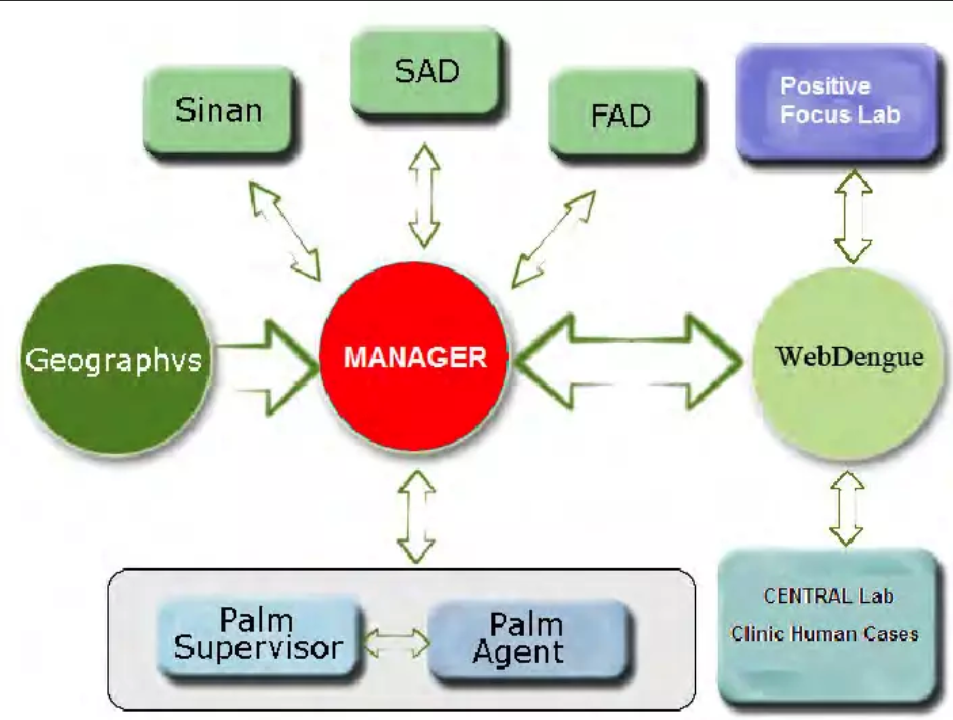
\includegraphics[width=12cm]{figuras/webdengue.png}
	}{
		\Fonte{Sistema WebDengue \cite{webdengue2011} }
	}
\end{figure}


O WebDengue \cite{webdengue2011}, possui nativamente uma base de dados organizada em um Banco de Dados espaço-temporal, que permite aos gestores realizarem diversas avaliações analíticas, de modo que se possa obter o melhor resultado no tratamento epidemiológico das arboviroses. Modelos estatísticos de previsão usando técnicas padrão (Médias Móveis, suavização exponencial, \emph{holt-winters} e outras), fazem parte do \emph{framework}. Apesar disto, notou-se que tais modelos não ajudam muito no processo de acompanhamento da dinâmica da expansão das arboviroses, pois não identificam nos bairros as áreas mais afetadas e que devem ser trabalhadas pelos agentes no sentido de debelar tais doenças.

A tarefa de agrupamento depende muito das características específicas dos dados e a maneira como eles são relacionadas. A Figura \ref{fig:st-types} exibe uma possível classificação de tais tipos de dados, com base na dimensão temporal, que descreve em que medida a evolução do objeto é capturada pelos dados, e a dimensão espacial, que descreve se os objetos estão associados a um local fixo ou sua localização é dinâmica e pode mudar no tempo.
Os tipos de dados espaço-temporais podem ser divididos em cinco categorias contendo eventos, variáveis georreferenciadas, séries temporais georreferenciadas, pontos em movimento e trajetórias. \citeautoronline{Kisilevich2009} descrevem as principais classes de tipos de dados:

\begin{figure}[!ht]
	\centering
	\Caption{\label{fig:st-types} Contexto para agrupamento espaço-temporal}	
	\UECEfig{}{
		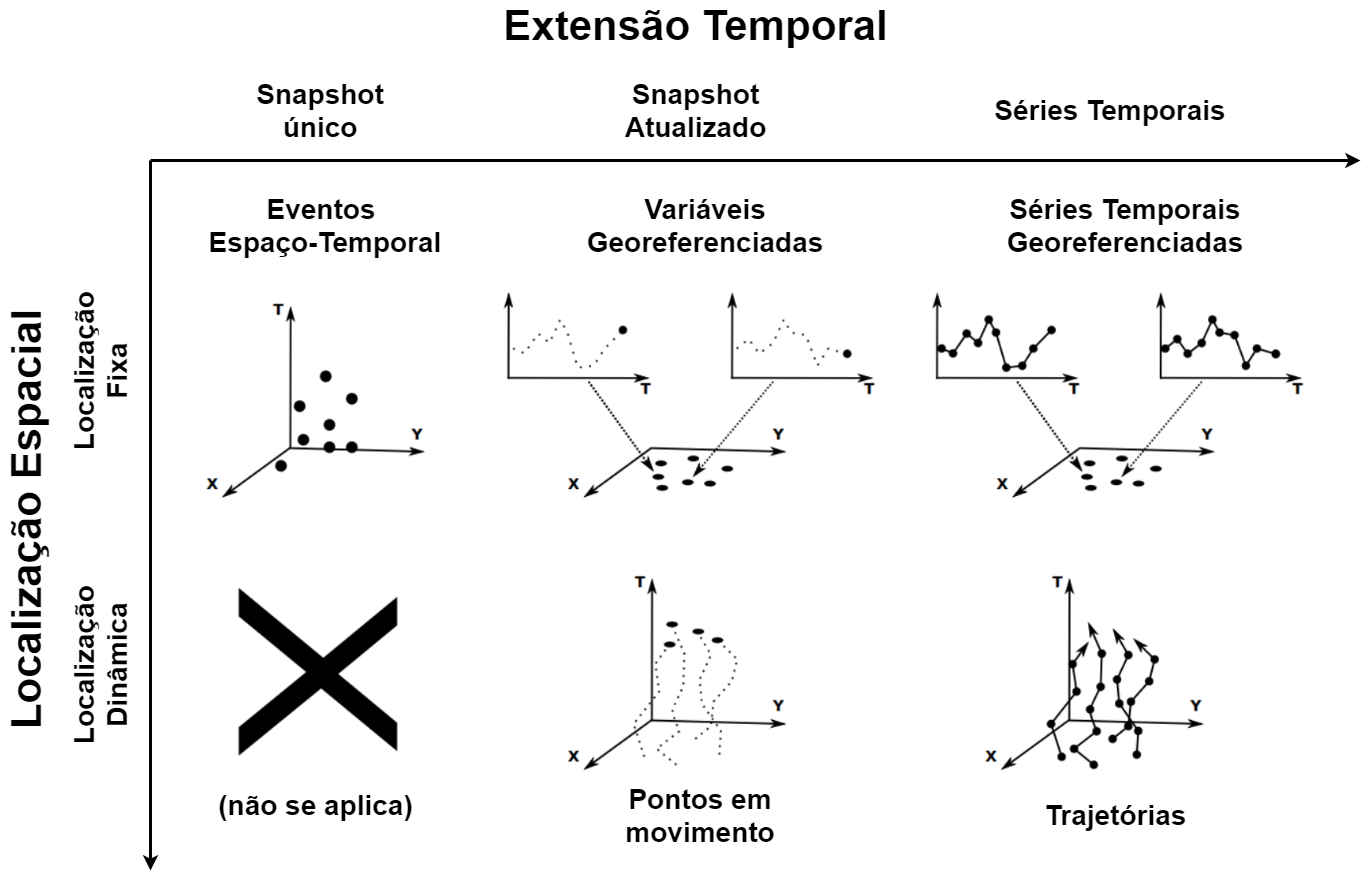
\includegraphics[width=15cm]{figuras/st-tipos.png}
	}{
		\Fonte{Elaborado pelo autor baseado em \cite{Kisilevich2009}}
	}
\end{figure}

\begin{itemize}
    \item Eventos Espaço-temporal: Um exemplo básico de informação espaço-temporal são os eventos espaço-temporais, como registros georreferenciados de uma epidemia. Cada evento é geralmente associado ao local onde foi registrado e ao registro de data e hora correspondente. Tanto a informação espacial quanto a temporal associada aos eventos são estáticas, uma vez que nenhum movimento ou qualquer outro tipo de evolução é possível. Encontrar grupos entre eventos significa descobrir que estão próximos no tempo e no espaço e possivelmente compartilham outras propriedades não espaciais. \citeautoronline{Birant2007STDBSCANAA} propuseram o algoritmo de agrupamento espaço-temporal \acrshort{ST-DBSCAN} que é uma extensão do algoritmo DBSCAN. Outro algoritmo para agrupamento espaço-temporal é o ST-IGN que é uma extensão do algoritmo IGN \cite{ign}. Esses dois algoritmos de agrupamento espaço-temporais foram implementados nesta dissertação para consolidar a metodologia proposta.
	\item Variáveis Georreferenciadas: quando é possível observar a evolução no tempo de alguns fenômenos em um local fixo, tem-se o que normalmente é chamado de uma variável georreferenciada, ou seja, o valor de mudança de tempo de alguma propriedade observada.
	\item Séries temporais georreferenciada: pode ser possível armazenar todo o histórico do objeto em evolução, fornecendo, portanto, uma série temporal (georreferenciada) para as variáveis medidas. Quando muitas variáveis estão disponíveis, elas geralmente são vistas como uma única série temporal multidimensional. Nesse caso, agrupando um conjunto de objetos requer comparar a maneira como a série temporal evolui e relacioná-la à sua posição espacial.
	\item Pontos em movimento: quando a localização espacial do objeto de dados está mudando no tempo. No caso mais simples, as informações disponíveis sobre esses objetos consistem em sua posição mais recente, como no contexto de monitoramento em tempo real de veículos.
	\item Trajetórias: descrevem o comportamento de movimento dos objetos e, portanto, o agrupamento pode ser usado para detectar grupos de objetos que se comportam de maneira semelhante.
\end{itemize}

% incluir referência para o grupo de pesquisa Data Mining e Categorização de Informações em Larga Escala?
Motivados pelo problema, o grupo de pesquisa em \textit{Data Mining e Categorização de Informações em Larga Escala}, desenvolveu uma concepção genérica de esforços no sentido de permitir a geração de modelos de previsão espaço-temporais da ocorrência de doenças provocadas por arbovisores. O primeiro passo nesse sentido foi dado com a criação de um modelo de visualização espaço-temporal robusto, denominado \emph{Dynagraph} \cite{dynagraph}, e o segundo seria a concepção, análise, implementação e avaliação de resultados de um \acrfull{SAD} que permita reconhecer agrupamentos de casos humanos de arboviroses, já que o mosquito se manifesta em concentrações definidas nas áreas urbanas de alta sucetibilidade à sua sobrevivência \cite{comportamentoDengue}.
Esta dissertação estuda o comportamento de métodos de agrupamento dinâmico espaço-temporais, considerando uma aplicação no monitoramento do avanço dos casos humanos de doenças provocadas por arboviroses (Dengue e Chikungunya) em Fortaleza/CE.

A representação dinâmica dos eventos também tem sido um problema importante. Muitos modelos são utilizados tais como representação espaço-temporal por vídeos e grafos. Na representação espaço-temporal por vídeos, o objetivo é sincronizar os modelos de previsão com a descoberta dos agrupamentos enquanto um vídeo real acontece (usado principalmente na climatologia \cite{faghmous2013}); já a representação dinâmica por grafos dinâmicos, tem sido estudada pela literatura com maior profundidade pois permite acompanhar eventos e gerar previsões espaço-temporais sabendo-se e controlando-se os principais atores do processo, tais como: elemento dinâmico e contexto dinâmico como descritos em \cite{holme:predictability} e \cite{Mitsa:2010}.

Ferramentas de grafos dinâmicos foram desenvolvidas e seguem em uso, como o Gephi \cite{gephi} e o Dynagraph \cite{dynagraph}. Aqui será feito um trabalho sobre o modelo Dynagraph para representação de uma estrutura dinâmica incluindo a possibilidade de variação dinâmica das características (cor, forma, tamanho, etc) dos elementos do grafo. Deste modo, esta visão evolutiva ajudaria ao modelo sistêmico representar claramente a realidade da evolução dos fenômenos que se deseja demonstrar para facilitar a tomada de decisão.

% Objetivos

Esta dissertação propõe e apresenta um \acrshort{SAD} especializado na previsão de agrupamentos dinâmicos espaço-temporais. Utilizando dados provenientes de bases oficiais do município de Fortaleza/CE, \acrfull{SIMDA}, advindas do monitoramento da evolução de doenças provocadas por arboviroses (Dengue e Chikungunya). 

% Objetivos Específicos}
Para que se alcance este objetivo, as seguintes etapas foram estabelecidas:

\begin{alineas}
    \item Descrever os tipos de agrupamentos dinâmicos.
	\item Extrair de características de previsão espaço-temporal sobre a evolução dos agrupamentos dinâmicos.
	\item Avaliar os resultados da metodologia de preparação de informações, parametrização e aplicação dos métodos de agrupamento são avaliados sobre estas bases de dados reais.
\end{alineas}

% Justificativa e Relevância

Em \acrshort{SIMDA}, estão disponíveis dados espaço-temporais para acompanhar a evolução da dengue e chikungunya em Fortaleza, que é um sistema para monitorar diariamente os casos de endemias como zika, leishmaniose, leptospirose, dengue e chikungunya. Somente estas duas últimas endemias estão disponíveis visualmente num mapa. As informações nesse sistema pouco ajudam na melhor tomada de decisão para direcionamento dos recursos apropriados para o controle das doenças nos períodos de grande crescimento. A antevisão do processo mostra a possibilidade de tornar factível a tomada de decisão assertiva. É preciso também saber o quão preciso é o método, para que seja usado como ferramenta de decisão neste contexto.

Existe a necessidade de ferramentas e estudos relacionando os assuntos abordados: agrupamento, previsão em dados dinâmicos espaço-temporais, grafos dinâmicos e sistemas web de forma integrada, bem como acelerar técnicas avançadas de agrupamento em grafos dinâmicos para esse tipo de tomada de decisão.

A pesquisa analisa dados extraídos para apoio à tomada de decisão, concentrando-se na avaliação dos resultados sobre bases de dados dinâmicas relativas a casos de Dengue e Chikungunya, tomando-se como base as características de evolução dos casos da doença observados entre 2016 e 2019 em Fortaleza/CE.

% Hipóteses
As hipóteses a seguir conduziram a elaboração desta dissertação:
\begin{alineas}
    \item É viabilizado o armazenamento dos dados por uma ferramenta de extração e armazenamento de dados automatizada seguindo a estrutura de dados do Dynagraph.
	\item É exequível a integração de um editor de características ao Dynagraph, que é um software extensível.	
	\item É realizável a utilização do modelo proposto de agrupamentos em grafos dinâmicos em um ambiente Web.	
	\item É possível a criação de um algoritmo capaz de sugerir agrupamentos naturais dinâmicos espaço-temporais de casos de doenças como dengue e chikungunya geolocalizados no tempo.
	\item É possível a avaliação da acertividade da metodologia no tocante do monitoramento da evolução da doença.
\end{alineas}

% Metodologia

Esta dissertação usou como fontes principais de pesquisa \textit{sites} especializados em artigos científicos, por exemplo, o portal de periódicos da \acrshort{CAPES}, \acrshort{IEEE}, Scielo e outros sites relevantes de referências que possuem livros, periódicos e dissertações disponíveis.

Os temas essenciais abordados nesta pesquisa foram:
\begin{itemize}
	\item Estrutura de dados em grafos dinâmicos.
	\item Algoritmos de agrupamentos dinâmicos.
	\item Modelos de previsão espaço-temporais.
	\item Sistemas de apoio a decisão web com \emph{Datawarehouse}.
\end{itemize}

No trabalho proposto, buscou-se inicialmente extrair informações baseadas na previsão de agrupamentos dinâmicos em grafos. Assim sendo, e após obter os dados a partir do \acrshort{SIMDA}, através de uma ferramenta implementada que automatiza a extração e armazenamento dos dados (concepção em apêndice), detectou-se a necessidade de um software para representação e tratamento de grafos dinâmicos, que tem como característica a extensibilidade. Para isso, foi escolhido e ajustado o software Dynagraph, \cite{dynagraph}.

Para a obtenção das informações espaço-temporais mapeáveis e características do indivíduo, seguem-se três estratégias para resolução do problema: na primeira os dados são analisados como um só grupo (Agrupamento Estático); na segunda os dados são tratados por intervalos pré-definidos; na terceira mapeia-se as evoluções entre intervalos observados.

Dessa forma, esta pesquisa visa indicar os possíveis grupos relacionados espacial e temporalmente.

Por fim, foi desenvolvido um modelo capaz de representar agrupamentos e previsão dinâmicos a partir do software Dynagraph, para avaliação e conclusão dos resultados obtidos em bases dinâmicas.

% Organização do Texto

Esta dissertação está organizada em 5 capítulos. O capítulo 1 apresenta uma
introdução à necessidade da representação e manipulação do agrupamento espaço-temporal dinâmico, assim como a previsão da formação de novos grupos dinâmicos. O capítulo 2 constitui a revisão bibliográfica sobre modelagem com grafos dinâmicos, métodos de agrupamento por densidade, redes dinâmicas, o Dynagraph, um editor de características e um conjunto de trabalhos relacionados a esta área de conhecimento. O capítulo 3 apresenta o modelo de agrupamento e previsão em redes dinâmicas. O capítulo 4 destaca
os resultados e comparação dos algoritmos apresentados. O capítulo 5 apresenta as conclusões, dificuldades encontradas/impedimentos e propostas de trabalhos futuros.









	\chapter{Conceitos e revisão bibliográfica}
\label{chap:estadodaarte}

Uma visão geral sobre agrupamentos é apresentada na seção \ref{agrupamentos}. Na seção \ref{dbscan} apresenta-se o algoritmo DBSCAN em detalhes e suas características. A seção \ref{stdbscan} apresenta o ST-DBSCAN, que é utilizada nesse trabalho para auxiliar os métodos de previsão dinâmica. Na seção  \ref{chap:redes-dinamicas}  discute-se redes dinâmicas e exibe-se o modelo Dynagraph e um editor de características. A seção  \ref{chap:trabalhos-relacionados}  define e apresenta os trabalhos relacionados ao problema de agrupamentos dinâmicos.

\section{Agrupamentos}
\label{agrupamentos}

A técnica de agrupamento, também chamada de \textit{clustering}, é uma das técnicas de mineração de dados mais comuns e é usada para descobrir padrões de distribuição nos dados. O agrupamento é feito com base na similaridade das características e na posição dos objetos. Dessa maneira, o objetivo é que os objetos do mesmo grupo sejam muito similares entre si e muito diferentes dos objetos de outros grupos.

Essa técnica é muito utilizada para dados estáticos. No entanto, há poucos trabalhos no âmbito espaço-temporal onde os dados estão na forma de campos espaço-temporais contínuos e os agrupamentos são dinâmicos. Além disso, os dados espaço-temporais originados por satélites em órbita terrestre, telefones celulares e outros sensores tendem conter muitos ruídos, são incompletos e heterogêneos, tornando sua análise especialmente desafiadora \cite{faghmous2013}.

Agrupamentos dinâmicos podem mudar seu tamanho, forma, localização e propriedades estatísticas de um tempo para o próximo. Embora os agrupamentos possam se mover ou mudar de forma, existem vários pontos que não alteram as associações de grupos por um período de tempo. Tendo isso em vista é possível extrair de forma autônoma agrupamentos dinâmicos em dados espaço-temporais contínuos que podem conter valores, ruídos ou características muito variáveis.

Existem muitas variações quanto à formação de grupos. Pode-se querer definir grupos a partir de um processo onde é dado o número desejado de partições a serem aplicadas entre os objetos a serem agrupados; pode-se querer definir quais são os grupos que naturalmente se formam dentro de um conjunto dado de objetos; pode-se querer classificar objetos a partir de classes de objetos já conhecidas; e por fim pode-se querer identificar objetos que não correspondem a nenhum grupo. 

Em processos de agrupamento dinâmico é necessário conhecer como os objetos se agrupam naturalmente assim como identificar os objetos que não estão associados a qualquer desses grupo.

Os métodos mais tradicionais para esses casos estão na classe dos métodos denominados particionais e hierárquicos. Alguns algoritmos de agrupamento integram as idéias de vários outros, logo é difícil classificar um algoritmo pertencendo a somente uma categoria de métodos de agrupamento. Além do que, algumas aplicações podem ter critérios que necessitam a integração de várias técnicas de agrupamento. Os principais métodos de agrupamento existentes na literatura são categorizados, como mostram as próximas sessões.

\subsection{Métodos baseados em particionamento}
A ideia principal desta classe de algoritmos de agrupamentos é criar ${K}$ grupos dos dados, onde ${K}$ é inserido pelo usuário.
Esse método consiste em escolher ${K}$ objetos como sendo os centros dos ${K}$ grupos.
Os objetos são divididos entre os ${K}$ grupos de acordo com algum critério de similaridade
estabelecido pelo algoritmo, de modo que cada objeto fique no grupo que tem o menor valor de
distância entre o objeto e o centro do grupo a que ele pertence.
Os algoritmos de particionamento são muito populares devido à sua facilidade de implementação e baixo custo computacional; no entanto, eles têm essas desvantagens: (1) eles são sensíveis à presença de ruído e \textit{outliers}, (2) eles podem descobrir apenas grupos com formas convexas e (3) o número de grupos precisa ser especificado.


\subsubsection{Agrupamentos K-Médias}
O algoritmo de agrupamento k-médias é uma das técnicas mais conhecidas dessa abordagem e foi introduzido por \cite{Macqueen67}. Ele utiliza a média dos objetos que são do grupo em questão, também conhecido como centro geométrico do grupo. A idéia principal neste algoritmo é usar a média dos objetos para atribuí-los a grupos e também usá-los para  representá-los.
K-médias é um algoritmo que garante a convergência para um ótimo local, mas não necessariamente um ótimo global. À medida que ${K}$ aumenta, o custo de encontrar a solução ótima diminui, e atinge seu mínimo quando ${K}$ é igual ao número de objetos \cite{Wu2008}. Especificamente, o procedimento é mostrado abaixo:
 \begin{enumerate}
	\item Inserir os objetos para serem agrupados e também o número ${K}$ de grupos.
	\item Escolher aleatoriamente os ${K}$ objetos como centro dos grupos originais.
	\item Atribuir cada objeto ao grupo com a média mais próxima.
	\item Calcular a nova média de cada grupo.
	\item Repetir a partir do passo 3.
	\item Parar quando o critério de convergência estiver satisfeito. O critério mais frequentemente usado, é a minimização do erro quadrático, dado por: 
	\begin{equation}
	E = \sum_{i=1}^{k}\sum_{o\in C_{i}} |o - \mu_{i}|^{2}
	\end{equation}
	onde ${o}$ é o ponto no espaço representando um dado objeto, ${\mu_{i}}$ é o representante do grupo ${C_{i}}$,
	 e ${K}$ o número de grupos.
\end{enumerate}

A seguir um exemplo do funcionamento do algoritmo na figura \ref{fig:kmedias}. Os objetos são mostrados como pontos e os centróides dos grupos são mostrados como cruzes. Na etapa \ref{fig:kmedias}-(a) encontra-se o conjunto de dados original. Em \ref{fig:kmedias}-(b) os centróides dos grupos são escolhidos aleatoriamente. De \ref{fig:kmedias}-(c) até \ref{fig:kmedias}-(f) ilustra a execução de duas iterações do k-médias. Em cada iteração, atribui-se cada objeto ao centróide mais próximo. Em seguida, cada centróide é movido para a média dos pontos atribuídos a ele.
\begin{figure}[!ht]
	\centering
	\Caption{\label{fig:kmedias} K-médias}	
	\UECEfig{}{
		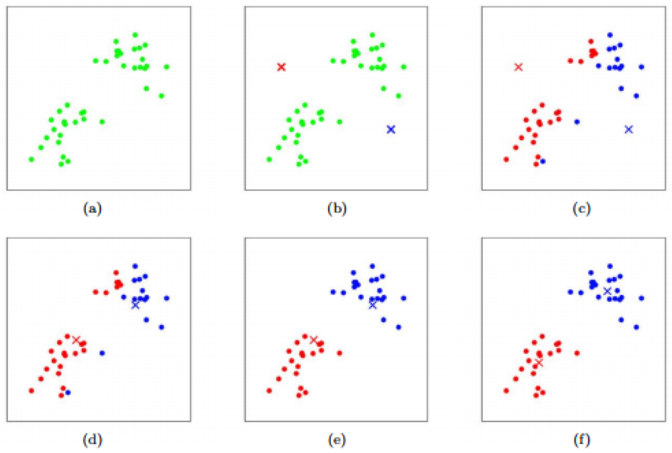
\includegraphics[width=14cm]{figuras/k-medias.png}
	}{
		\Fonte{\cite{kmedias:exemplo}}
	}
\end{figure}

\subsubsection{Agrupamentos K-Medoids}
O algoritmo de \textit{K-Medoids} ou K-medianas foi introduzido primeiramente em \cite{kaufmann1990}. Seu objetivo é particionar os objetos em ${k}$ grupos, previamente conhecidos, tal que a soma das distâncias entre cada objeto e a mediana do seu grupo seja mínima. Nesse algoritmo, cada grupo é representado pelo objeto mais próximo ao centro, conhecido também por \textit{medoid}.
O processo geral para o algoritmo é o seguinte:
 \begin{enumerate}
 	\item Escolher aleatoriamente ${k}$ objetos como os \textit{medoids} iniciais.
 	\item Atribuir cada um dos objetos restantes ao grupo que com o \textit{medoid} mais próximo.
 	\item Em um grupo, selecionar aleatoriamente um objeto que não seja \textit{medoid} (${nonmedoid}$), que será referenciado como ${O_{nonmedoid}}$.
 	\item Calcular o custo de substituir o \textit{medoid} com ${O_{nonmedoid}}$. Este custo é a diferença do erro quadrático se o \textit{medoid} atual for substituído por ${O_{nonmedoid}}$. Se for negativo, fazer ${O_{nonmedoid}}$ o \textit{medoid} do grupo. O erro quadrático é novamente somado ao erro de todos os objetos:
 	\begin{equation}
 	E = \sum_{i=1}^{k}\sum_{o\in C_{i}} |o - O_{medoid(i)}|^{2}
 	\end{equation}
 	onde ${O_{medoid(i)}}$ é o \textit{medoid} do grupo ${C_{i}}$.
 	\item Repetir a partir do passo 2 até que não haja mudanças. 
 \end{enumerate}

Um exemplo é dado nas figuras \ref{fig:kmedianaA} e \ref{fig:kmedianaB}, onde nove objetos são distribuídos em dois grupos, portanto dois \textit{medoids}. Os objetos azuis correspondem aos \textit{medoids}, os segmentos de reta são as distâncias implícitas ao medoid de cada grupo, e os valores S1 e S2 são às somas das distâncias dos objetos aos seus respectivos \textit{medoids}. Nota-se que a figura \ref{fig:kmedianaB} representa a melhor solução, pois a soma total é igual a 300.

\begin{figure}[!ht]
	\centering
	\Caption{\label{fig:kmedianaA} K-mediana (a)}	
	\UECEfig{}{
		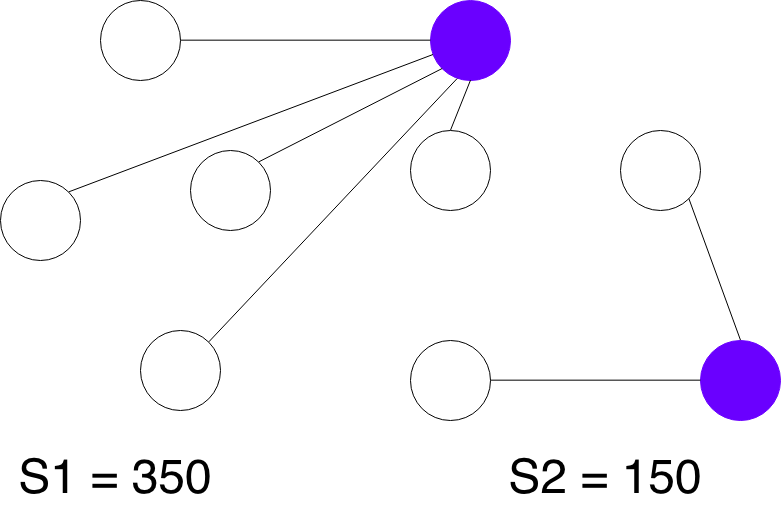
\includegraphics[width=7cm]{figuras/k-mediana-a.png}
	}{
		\Fonte{Elaborado pelo autor}
	}
\end{figure}
\begin{figure}[!ht]
	\centering
	\Caption{\label{fig:kmedianaB} K-mediana (b)}	
	\UECEfig{}{
		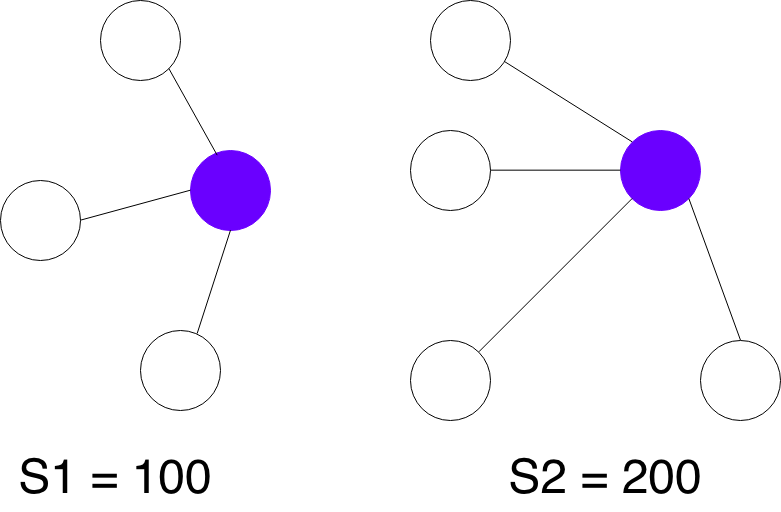
\includegraphics[width=7cm]{figuras/k-mediana-b.png}
	}{
		\Fonte{Elaborado pelo autor}
	}
\end{figure}

\subsection{Métodos Hierárquicos}
Nesta classe de algoritmos os objetos são colocados em uma hierarquia que é percorrida de baixo para cima (\textit{bottom-up}) ou de cima para baixo (\textit{top-down}) para criar os grupos. A vantagem deste tipo de agrupamento é que ele não requer nenhum conhecimento sobre o número de grupos, e a desvantagem é sua complexidade computacional \cite{Lin2004}. Muitas vezes, uma estrutura em árvore, um dendrograma, é usada para representar os níveis hierárquicos aninhados.

Os métodos aglomerativos funcionam de uma maneira \textit{bottom-up},
assumindo inicialmente que cada elemento do conjunto de dados representa um grupo. Em seguida, os grupos são fundidos em grupos maiores até a criação de um grupo único ou qualquer outro critério de parada.

A abordagem divisiva trabalha de maneira \textit{top-down}, considerando todo o conjunto de dados como um só grupo, que é dividido de maneira recursiva de acordo com a medida (métrica) de similaridade estabelecida.

\subsubsection{O algoritmo BIRCH}
\label{sub:birch}

Em \cite{Zhang1996}, BIRCH significa balanceamento interativo com redução e agrupamento usando hierarquias - \emph{Balanced Iterative Reducing and Clustering using Hierarchies}. Ele é um algoritmo usado para agrupamentos em bases de dados muito grandes sendo considerado um dos métodos hierárquicos mais utilizados pela literatura. As vantagens do BIRCH são as seguintes:

\begin{itemize}
	\item BIRCH trabalha de maneira local. Isso é obtido usando medições que indicam a proximidade natural dos pontos, de modo que cada decisão de agrupamento possa ser feita sem verificar todos os pontos de dados ou grupos existentes.
	\item Leva em conta a estrutura de dados espacial. Ele trata os pontos em uma região densa como um único grupo, enquanto os pontos em uma região esparsa são caracterizados como \textit{outliers} e podem ser removidos opcionalmente.
	\item O algoritmo faz uso da memória disponível enquanto minimiza os custos de Entrada/Saída de dados.
\end{itemize}

Os principais conceitos do BIRCH, que funcionam de maneira incremental são: o Agrupamento por Característica (AC) e AC-árvore. Onde AC consiste em tomar todas as informações que precisam ser mantidas sobre um grupo. Já o AC-árvore é utilizado para representar a hierarquia de grupos.

A estrutura da AC-árvore é exibida na figura \ref{fig:birch} e descrita a seguir.

\begin{itemize}
    \item Cada nó que não é folha tem no máximo ${B}$ entradas;
    \item Cada nó folha tem no máximo ${L}$ AC entradas que satisfazem o limite ${T}$, que é o diâmetro máximo de raio;
    \item P (tamanho da página em bytes) é o tamanho máximo de um nó;
    \item Compacto: cada nó da folha é um subgrupo, não um ponto de dados;
\end{itemize}

\begin{figure}[!ht]
	\centering
	\Caption{\label{fig:birch} Estrutura de uma AC-árvore}	
	\UECEfig{}{
		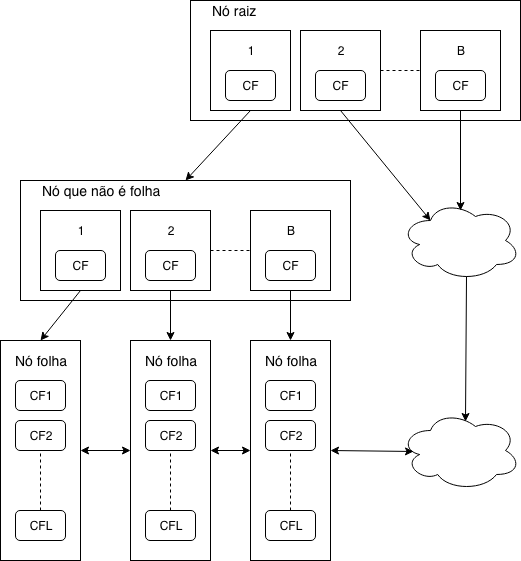
\includegraphics[width=14cm]{figuras/Birch.png}
	}{
		\Fonte{Elaborado pelo autor}
	}
\end{figure}

O agrupamento acontece essencialmente em duas fases. Na primeira delas, o algoritmo lê o conjunto de dados e constrói uma AC-árvore inicial. Essa árvore é utilizada para representar a hierarquia dos grupos. Na segunda fase, um algoritmo de agrupamento selecionado é aplicado às folhas da AC-árvore, removendo grupos esparsos e agrupando os mais densos em grupos maiores.

O algoritmo BIRCH é descrito como segue:

\begin{enumerate}
    \item Carregar os dados na memória através da construção de uma AC-árvore;
        \begin{enumerate}
            \item Escolher um valor inicial de entrada, começar inserindo os pontos de dados um por um na árvore conforme o algoritmo de inserção;
            \item Se, no meio da etapa acima, o tamanho da AC-árvore exceder o tamanho da memória disponível, aumentar o valor do limite;
            \item Converter a árvore parcialmente construída em uma nova árvore;
            \item Repetir as etapas acima até que todo o conjunto de dados seja verificado e uma árvore completa seja criada;
            \item Manipulação dos \textit{outliers};
        \end{enumerate}
    \item Condensar a AC-árvore anterior em uma menor;
        \begin{enumerate}
            \item Criar uma AC-árvore menor aumentando o limite;
            \item Remover mais \textit{outliers};
        \end{enumerate}
    \item Agrupamento global;
        \begin{enumerate}
            \item Aplicar o algoritmo nos dados de entrada da AC-árvore;
            \item Melhorar a qualidade dos grupos;
        \end{enumerate}    
    \item Aprimoramentos do agrupamento;
        \begin{enumerate}
            \item Verificar todo o conjunto de dados para rotular os pontos de dados;
            \item Manipulação dos \textit{outliers};
        \end{enumerate}    
\end{enumerate}

Um exemplo do Birch é dado a seguir na figura \ref{fig:birch01}. Após a inserção do subgrupo AC8 em LN1, e se o fator de ramificação de um nó folha não puder exceder 3, então o LN1 é dividido, como exibe a figura \ref{fig:birch02}. Se o fator de ramificação de um nó que não é folha não puder exceder 3, a raiz é dividida e a altura da AC-árvore aumenta em um, como mostra a figura \ref{fig:birch03}.

\begin{figure}[!ht]
	\centering
	\Caption{\label{fig:birch01} Exemplo algoritmo de Birch - Novo subgrupo}	
	\UECEfig{}{
		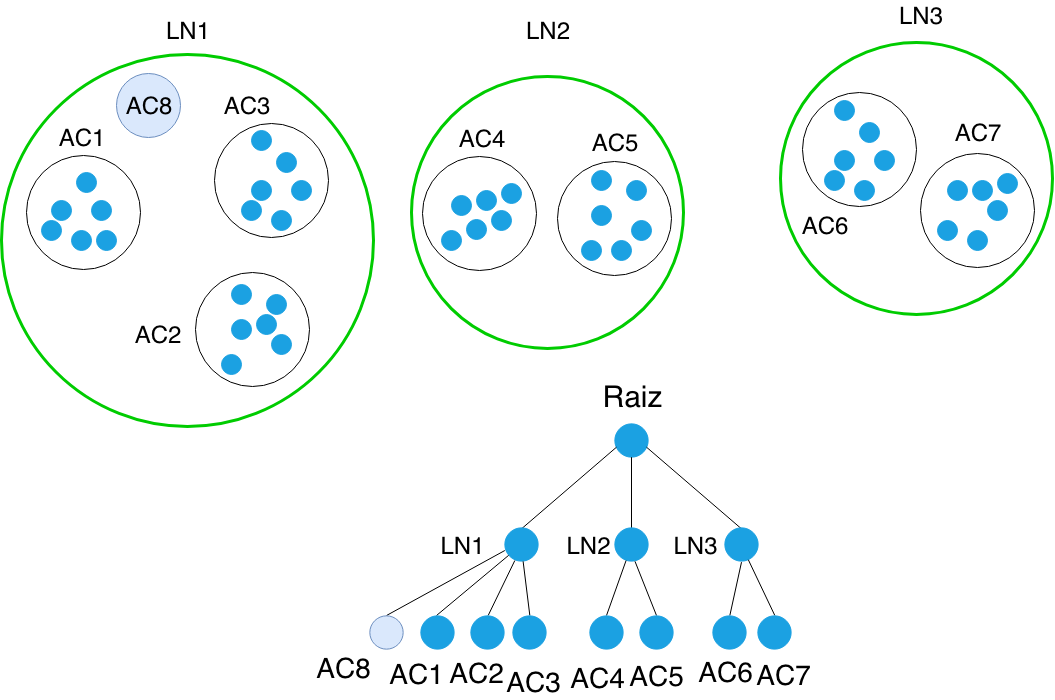
\includegraphics[width=14cm]{figuras/Birch01.png}
	}{
		\Fonte{Elaborado pelo autor}
	}
\end{figure}

\begin{figure}[!ht]
	\centering
	\Caption{\label{fig:birch02} Exemplo algoritmo de Birch - Operação de inserção parte 1}	
	\UECEfig{}{
		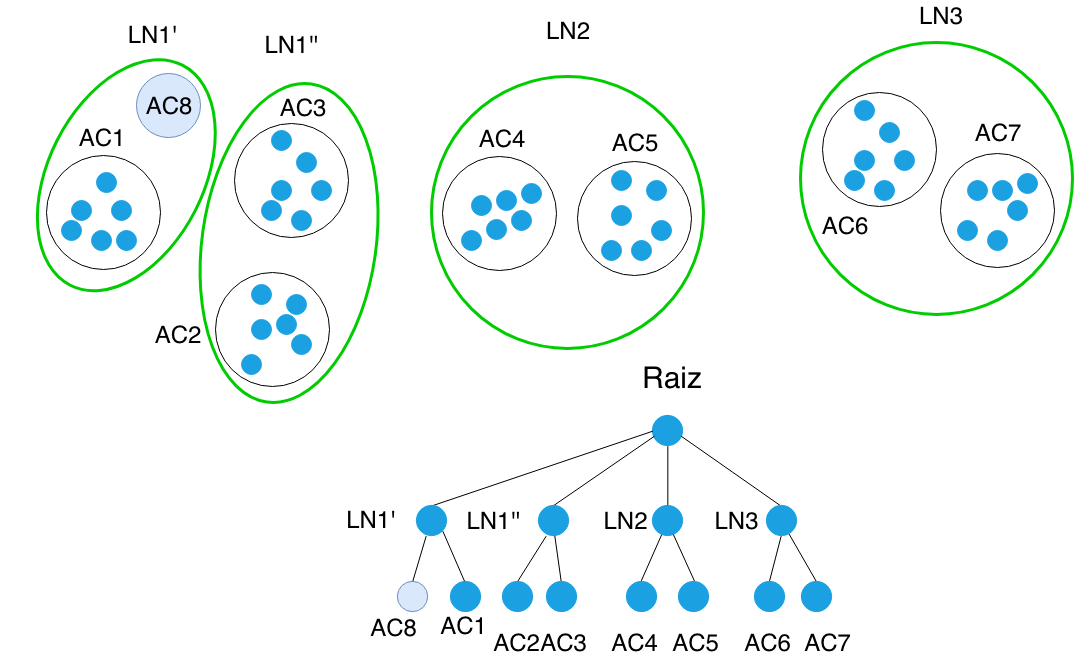
\includegraphics[width=14cm]{figuras/Birch02.png}
	}{
		\Fonte{Elaborado pelo autor}
	}
\end{figure}

\begin{figure}[!ht]
	\centering
	\Caption{\label{fig:birch03} Exemplo algoritmo de Birch - Divisão da raiz}	
	\UECEfig{}{
		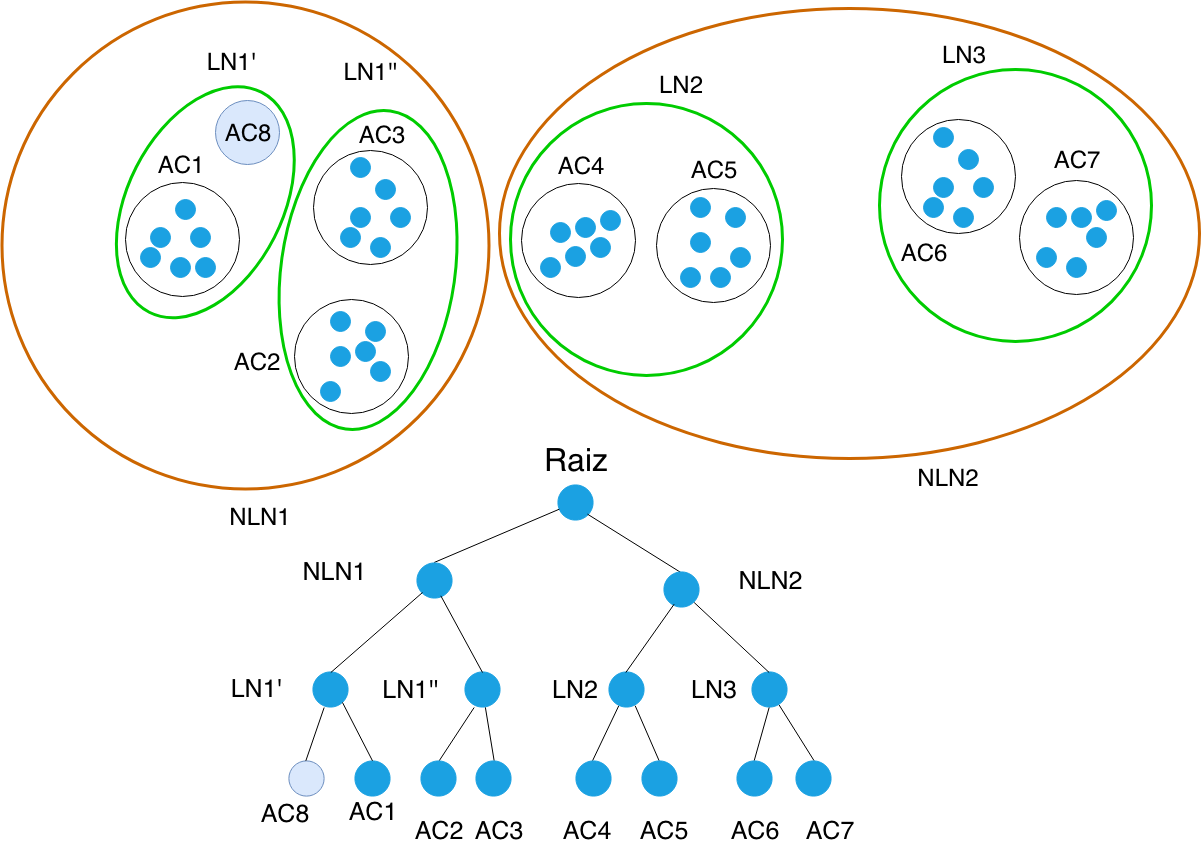
\includegraphics[width=14cm]{figuras/Birch03.png}
	}{
		\Fonte{Elaborado pelo autor}
	}
\end{figure}

\subsubsection{O algoritmo CURE}
Em \cite{Guha1998}, outro algoritmo hierárquico é proposto para detectar grupos que não são necessariamente convexos. Os grupos do CURE são representados por um número fixo de objetos bem espalhados que são encolhidos em direção ao centro do grupo por uma determinada fração. O CURE difere do algoritmo BIRCH de duas maneiras:
\begin{itemize}
\item O CURE começa desenhando uma amostra aleatória em vez de pré-agrupar todos os objetos de dados, como no caso do BIRCH.
\item O CURE primeiro particiona a amostra aleatória e, em seguida, em cada partição, os dados são parcialmente agrupados. Em seguida, os \textit{outliers} são eliminados e os dados pré-agrupados em cada partição são agrupados para gerar os grupos finais.
\end{itemize}
Os resultados experimentais no artigo mostram que o tempo de execução do CURE é sempre menor que o do BIRCH. Mais importante, os resultados mostram que, à medida que o tamanho do banco de dados aumenta, o tempo de execução do BIRCH aumenta rapidamente enquanto o tempo de execução do CURE aumenta muito pouco. O motivo disto é que o BIRCH varre todo o banco de dados e usa todos os objetos para o pré-agrupamento, enquanto o CURE usa apenas uma amostra aleatória.

As etapas do algoritmo CURE são:

\begin{enumerate}
    \item Seleção aleatória;
        \begin{enumerate}
            \item quando todo o conjunto de dados é considerado como entrada de algoritmo, o tempo de execução pode ser alto devido aos custos de I/O;
            \item para acelerar as operações do algoritmo, a amostragem aleatória é ajustada na memória principal;
        \end{enumerate}
    \item Particionamento;
        \begin{enumerate}
            \item Quando os grupos no conjunto de dados se tornam menos densos, a seleção aleatória com objetos limitados torna-se inútil, logo é necessário aumentar a amostragem aleatória;
            \item Cada grupo de objetos deve caber na memória principal para aumentar o desempenho do grupo parcialmente;
        \end{enumerate}
    \item Agrupamento parcial das partições;
        \begin{enumerate}
            \item Um número constante ${c}$ de objetos bem dispersos em um grupo é escolhido como representativo. Esses objetos capturam toda a forma possível que poderia ter o grupo;
            \item Os objetos são reduzidos em direção à média do grupo;
            \item Os grupos com o par de objetos representativos mais próximo são os grupos que são mesclados (merge) em cada etapa do CURE;
        \end{enumerate}
    \item Remoção dos ${outliers}$;
        \begin{enumerate}
            \item Os \textit{outliers}, devido à sua maior distância para outros objetos, tendem a se agrupar com outros objetos e geralmente crescem a uma taxa muito mais lenta do que os grupos atuais. Assim, o número de objetos em uma coleção de \textit{outliers} é normalmente muito menor que o número em um grupo.
        \end{enumerate}
    \item Agrupamento parcial dos grupos;
    \item Rotular dados no disco;
        \begin{enumerate}
            \item O processo de seleção aleatória do conjunto de dados inicial, exclui a maioria dos objetos.
            \item Estes objetos devem ser atribuídos a algum grupo criado em fases anteriores.
            \item Cada grupo criado é representado por uma fração de objetos selecionados aleatoriamente e cada objeto excluído na primeira fase é associado ao grupo cujo objeto representativo está mais próximo;
        \end{enumerate}
\end{enumerate}

As figuras \ref{fig:cureA}, \ref{fig:cureB}, \ref{fig:cureC} e \ref{fig:cureD} descrevem um exemplo do CURE.
\begin{figure}[!ht]
	\centering
	\Caption{\label{fig:cureA} CURE - amostra de dados}	
	\UECEfig{}{
		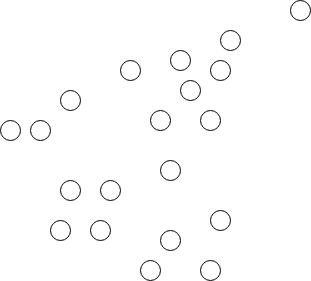
\includegraphics[width=6cm]{figuras/cureA.png}
	}{
		\Fonte{Elaborado pelo autor}
	}
\end{figure}
\begin{figure}[!ht]
	\centering
	\Caption{\label{fig:cureB} CURE - Três grupos com pontos representativos}
	\UECEfig{}{
		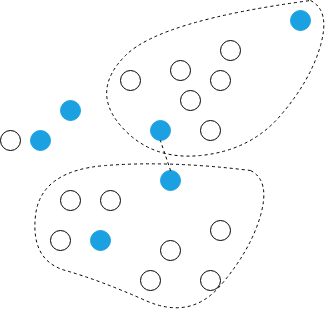
\includegraphics[width=6cm]{figuras/cureB.png}
	}{
		\Fonte{Elaborado pelo autor}
	}
\end{figure}
\begin{figure}[!ht]
	\centering
	\Caption{\label{fig:cureC} CURE - Merge dos grupos com pontos mais próximos}	
	\UECEfig{}{
		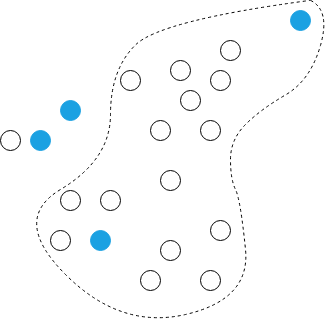
\includegraphics[width=6cm]{figuras/cureC.png}
	}{
		\Fonte{Elaborado pelo autor}
	}
\end{figure}
\begin{figure}[!ht]
	\centering
	\Caption{\label{fig:cureD} CURE - Encolhimento de pontos representativos}	
	\UECEfig{}{
		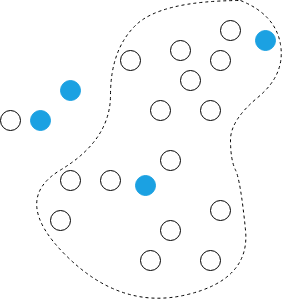
\includegraphics[width=6cm]{figuras/cureD.png}
	}{
		\Fonte{Elaborado pelo autor}
	}
\end{figure}

\subsubsection{Algoritmo de Kruskal}
Este algoritmo foi proposto em \cite{kruskal} e seu objetivo é encontrar um subconjunto das arestas que forma uma árvore geradora mínima que contém todos os vértices, onde a soma dos pesos das arestas da árvore é minimizada.

Seja ${G = (V, E)}$ um grafo convexo de ${V}$ vértices com o conjunto ${E}$ de arestas, o algoritmo de Kruskal inicia com T vazio e seleciona a aresta de ${E}$ que tem o menor peso e se ela conecta dois grupos distintos, então colocam-nas no conjunto ${T}$. Em seguida, os dois grupos formados se unem para formar um novo agrupamento, e se ela não conectar dois grupos diferentes, então a aresta é descartada. Com isso evita-se a formação de um ciclo. O algoritmo prossegue assim até obter um único grupo, neste caso ${T}$ constitui a solução.
Esse método é utilizado no algoritmo IGN apresentado na seção \ref{sub:ign} e seu funcionamento pode ser resumido nos seguintes passos:
\begin{enumerate}
    \item T = ${\varnothing}$;
    \item Para cada vértice ${v \in V[G]}$ criar as árvores;
    \item Colocar os arcos em ordem crescente de peso;
    \item Para cada arco $({u, v} \in E)$ verificar se ambos estão na mesma árvore. Senão, adicinar o arco em T e juntar os vértices nas duas árvores.
\end{enumerate}

A figura \ref{fig:kruskal} exibe os passos iterativos do algoritmo de Kruskal, que foi implementado no sistema SCLUSTER \cite{scluster}.

\begin{figure}[!ht]
	\centering
	\Caption{\label{fig:kruskal} Etapas iterativas do algoritmo de Kruskal}
	\UECEfig{}{
		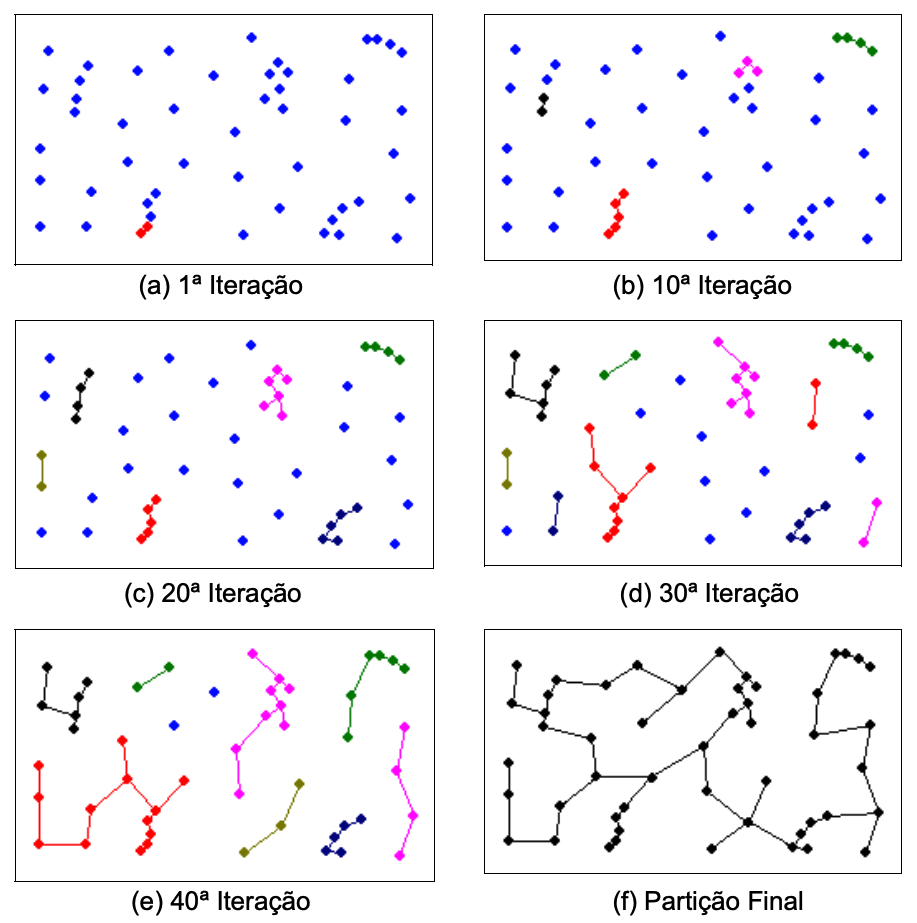
\includegraphics[width=14cm]{figuras/kruskal.png}
	}{
		\Fonte{\cite{joaoFrederico}}
	}
\end{figure}

\subsubsection{O algoritmo IGN}
 \label{sub:ign}
O IGN (Identificador de Grupos Naturais) \cite{ign} é baseado na construção de Árvore Geradora Mínima (AGM) sobre os dados do conjunto a classificar. Uma árvore geradora de um grafo conexo ${G = (V, E)}$ é uma estrutura em árvore ${T}$ que é um sub-grafo de ${G}$ e contém todos os vértices de ${G}$. Além disso, cada aresta ${e}$ possui um peso ${p(e)}$. Denomina-se peso de uma árvore geradora ${T=(V,E_T)}$ de ${G}$ a soma dos pesos das arestas ${E_T}$. Se um grafo é desconexo, não se pode identificar nenhuma árvore geradora. Mas pode-se identificar no mínimo uma floresta de árvores geradoras, uma para cada componente do grafo. Uma árvore geradora mínima é a árvore geradora de ${G}$ que possui peso mínimo dentre todas as árvores geradoras de ${G}$.
Este método é conceitualmente distinto dos demais, pois estabelece uma relação entre a construção da árvore hierárquica (árvore geradora mínima - AGM) e, de trás para frente, acompanhando a retirada dos elos (ligações entre classes) da árvore, o método evolui buscando a maior tangente da função de decaimento formada pelo custo de retirada das ligações da AGM.

O procedimento para identificar os grupos naturais para encontrar a melhor quantidade pode ser descrito a seguir:
 \begin{enumerate}
\item Executar o algoritmo de Kruskal guardando os custos dos grupos gerados. Iniciando de ${n}$ grupos até 1;
\item Encontrar o módulo da diferença entre o custo de cada iteração com os custos dos seus dois sucessores;
\item Selecionar a menor diferença entre o custo/valor da maior tangente obtido a cada iteração do passo anterior com o seu predecessor;
\item Retornar a composição das árvores do melhor resultado respeitando o parâmetro de quantidade mínima de elementos para se constituir um grupo.
\end{enumerate}

A complexidade do método IGN é ${O(n^2 log n)}$, onde ${n}$ é o número de indivíduos da base de dados. Após a execução do algoritmo de Kruskal, inicia os cortes nas árvores para as buscas dos grupos.
Algumas características desse método são:
\begin{itemize}
\item Apresenta bons resultados em qualquer métrica;
\item É sensível à presença de \emph{outliers} em situações muito específicas. Nestes casos pode apresentar resultados insatisfatórios quando houver proximidade de \emph{outliers} entre grupos naturalmente formados, confundindo os grupos naturais pela existência de "indivíduos pontes" (que surgem em função das dimensões de afastamento entre grupos inerentes);
\item Se há uma separação definida (um corte), o método é exato, ou seja, sempre encontrará os grupos naturais. Se a separação não existe, o método pode falhar;
\item Diferentemente dos demais, o número de grupos naturais e sua composição é obtida automaticamente no processo;
\item Usa o dendrograma de forma invertida para definir o ponto de corte (corte transversal no dendrograma), baseado na função monótona decrescente gerada pela função de custo de retirada das arestas da AGM (da maior para a menor) formada entre os indivíduos do processo de agrupamento.
\end{itemize}

Para facilitar as tarefas de análise multivariada, \cite{ign} desenvolveram o sistema SCLUSTER \cite{scluster}. Este \textit{software} é utilizado no exemplo seguinte apresentado em \cite{devillez}, onde um conjunto observado contém 236 pontos com duas variáveis, como exibe a figura \ref{fig:ignExemplo}. O resultado é a formação de quatro grupos, onde o primeiro possui 47 pontos, o segundo e o terceiro com 57, e o quarto com 41, além de 34 pontos do tipo \textit{outliers}.

\begin{figure}[!ht]
	\centering
	\Caption{\label{fig:ignExemplo} IGN - Grupo de dados com 4 grupos}	
	\UECEfig{}{
		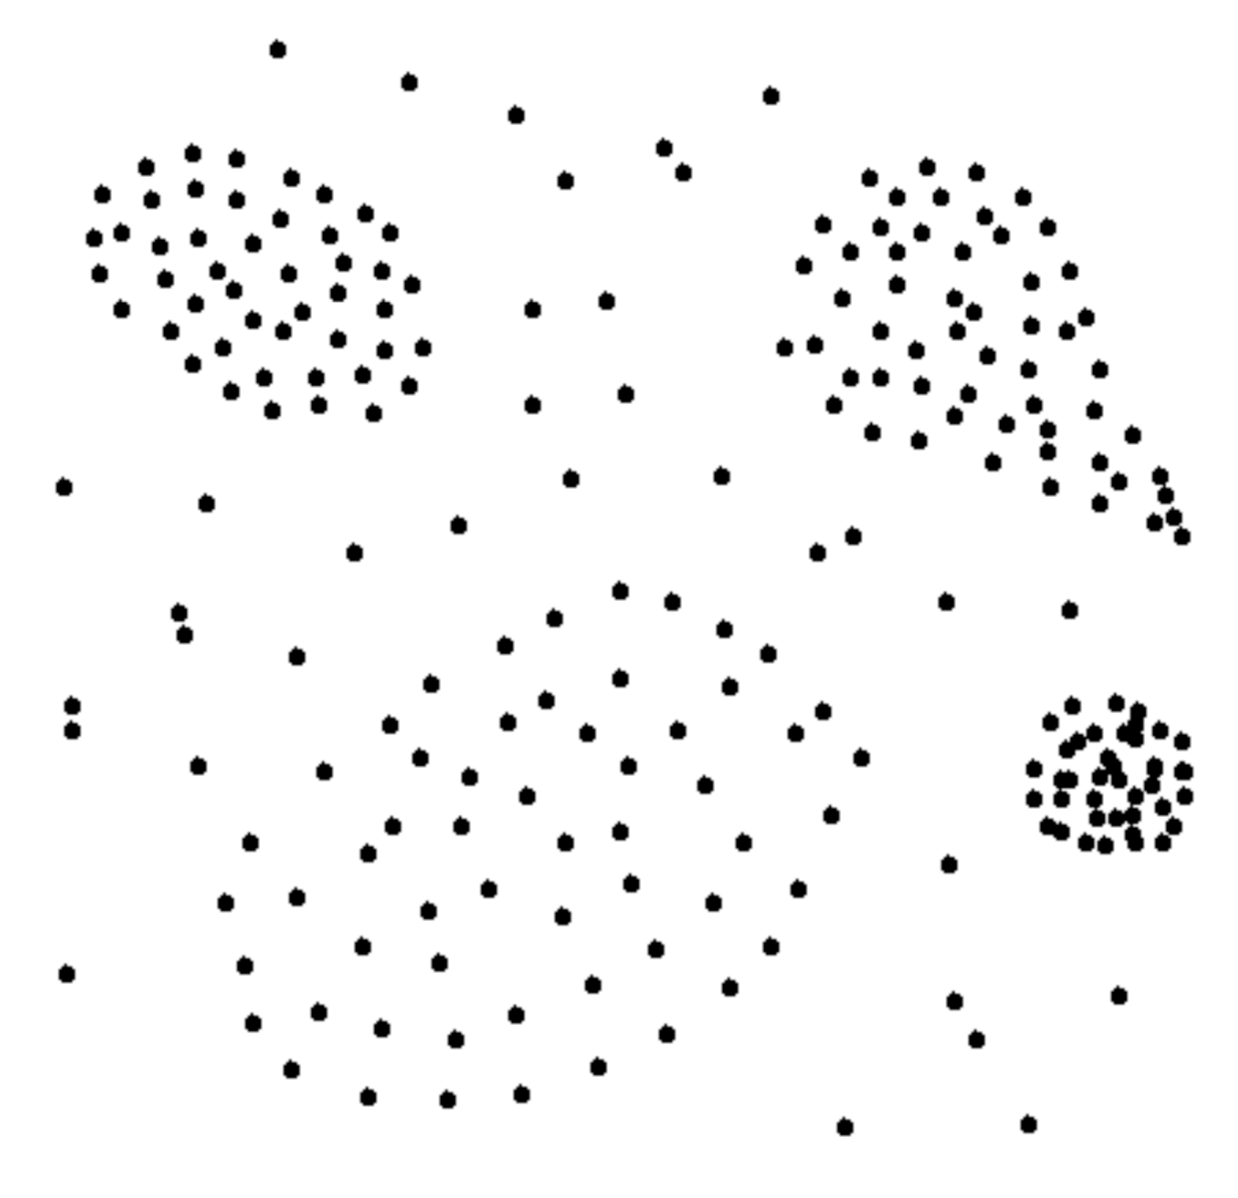
\includegraphics[width=10cm]{figuras/ignExemplo.png}
	}{
		\Fonte{\cite{joaoFrederico}}
	}
\end{figure}

Pode-se observar que os grupos foram identificados ao executar o algoritmo IGN separando os 236 pontos em quatro grupos, como mostrado na tabela \ref{tab:ignTabela} e figura \ref{fig:ignExemploResultado}.

\begin{table}[!ht]	
	\centering
	\Caption{\label{tab:ignTabela} IGN - Resultado para 4 grupos}
	\UECEtab{}{
		\begin{tabular}{|l|l|l|l|l|l|l|}
			\toprule
	    		Grupo & Grupo 01 & Grupo 02 & Grupo 03 & Grupo 04 & \textit{Outlier} & Total \\
			\midrule \midrule
				\begin{tabular}[c]{@{}l@{}}Pontos esperados por \\ grupo\end{tabular} & 47 & 57 & 57 & 41 & 34 & 236 \\
				\begin{tabular}[c]{@{}l@{}}Pontos alocados ao \\ grupo\end{tabular} & 47 & 57 & 57 & 41 & 34 & 236 \\
				\begin{tabular}[c]{@{}l@{}}Pontos alocados ao \\ grupo conforme o esperado\end{tabular} & 47 & 57 & 57 & 41 & 34 & 236 \\
				\begin{tabular}[c]{@{}l@{}}Pontos alocados ao \\ grupo diferente do esperado\end{tabular} & 0 & 0 & 0 & 0 & 0 & 0 \\
			\bottomrule
		\end{tabular}
	}{
		\Fonte{\cite{joaoFrederico}}
    }
\end{table}

\begin{figure}[!ht]
	\centering
	\Caption{\label{fig:ignExemploResultado} IGN - Agrupamento para 4 grupos}	
	\UECEfig{}{
		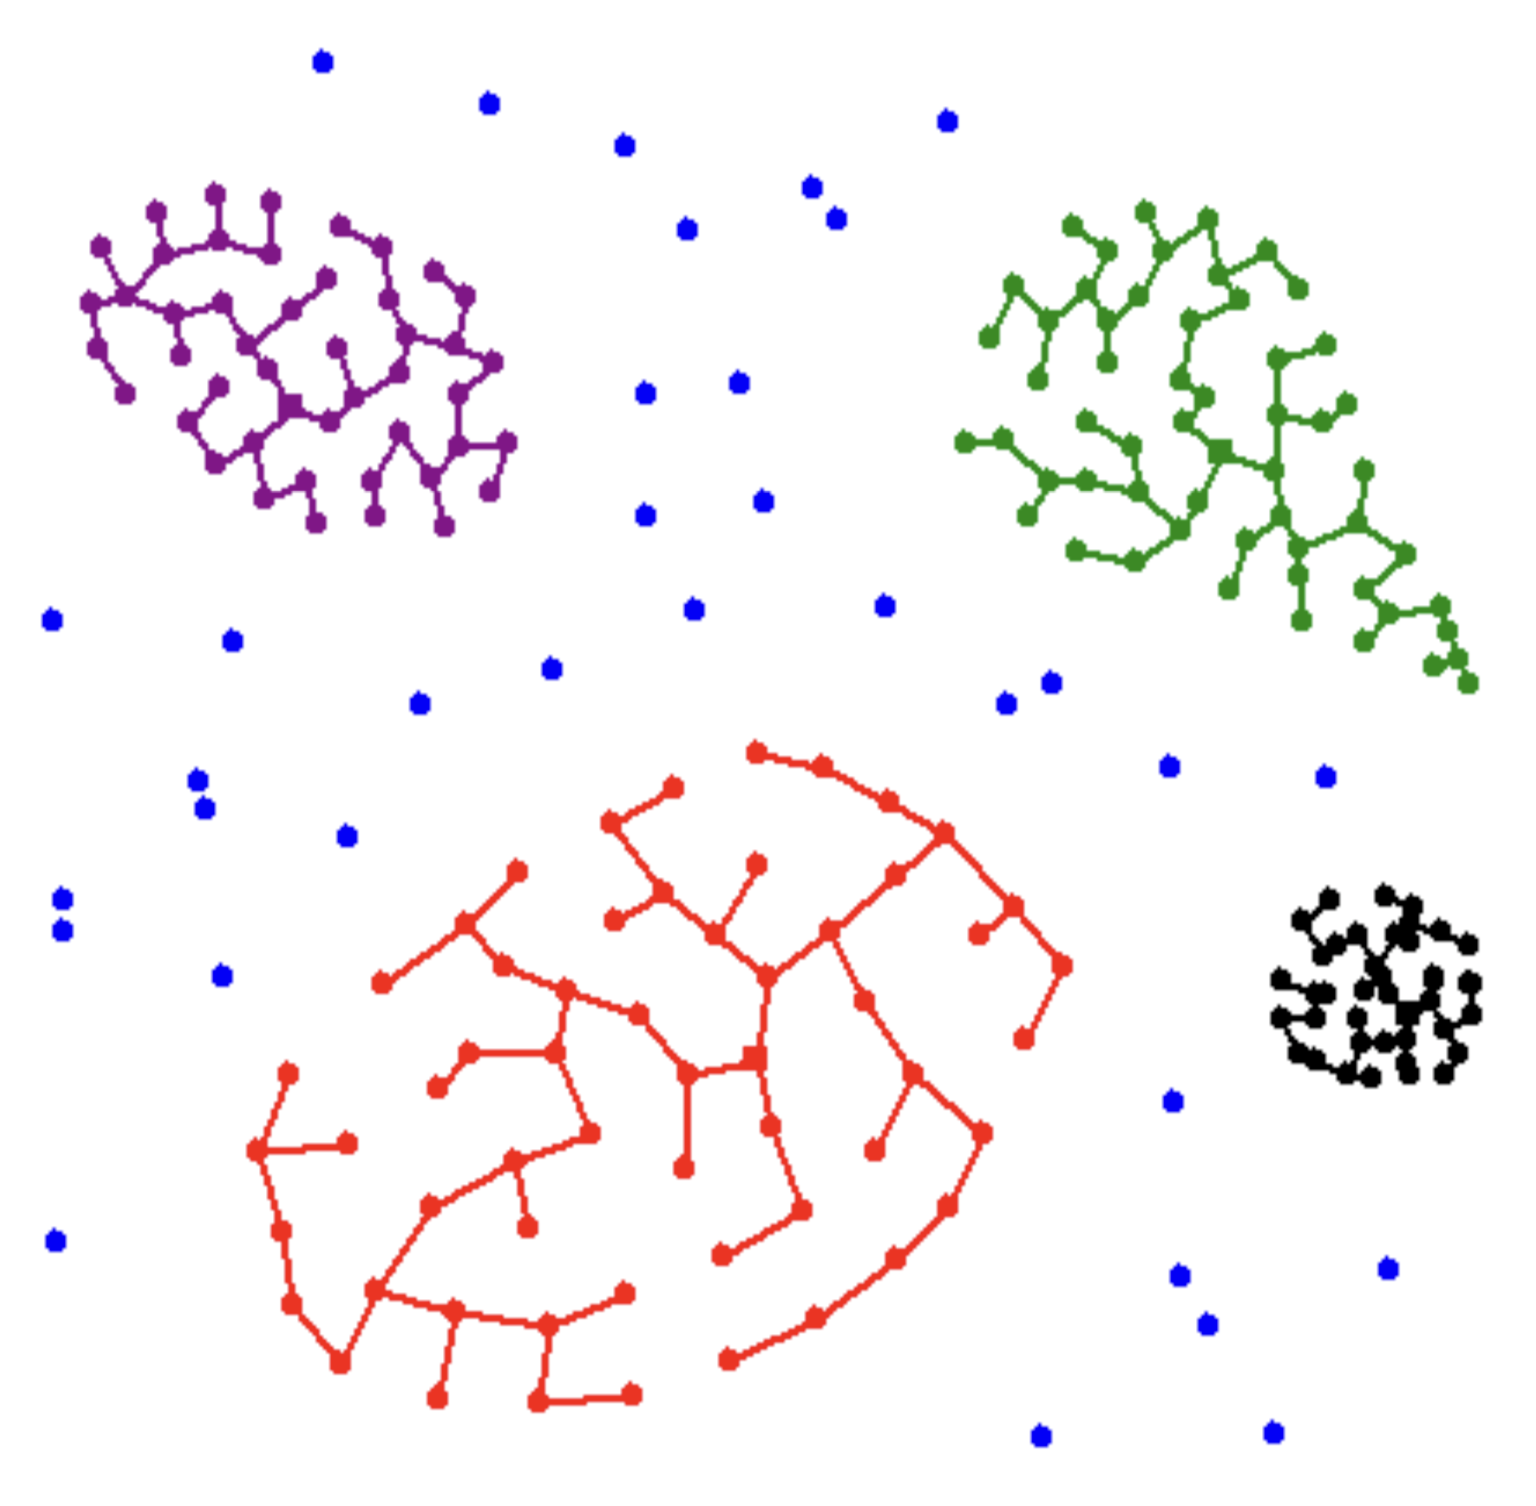
\includegraphics[width=10cm]{figuras/ignExemploResultado.png}
	}{
		\Fonte{\cite{joaoFrederico}}
	}
\end{figure}


\subsection{Métodos baseados em estrutura de grade}
Enquanto que os outros métodos de agrupamento discutidos são orientados aos dados, os métodos baseados em grade são orientados ao espaço. Essencialmente, o espaço é dividido em células retangulares, representadas por uma estrutura de grade hierárquica.

\subsubsection{O algoritmo STING}
\cite{Wang1997} propuseram um método de agrupamento baseado em grade, STING (\emph{STatistical INformation Grid} - Informação estatística baseada em grade), para agrupar bancos de dados espaciais e facilitar consultas orientadas à região. Esse algoritmo se baseia na construção de diversas camadas de grade, onde células de uma camada mais alta são subdivididas para a criação de células nas camadas mais baixas, como mostra a figura \ref{fig:sting}.

\begin{figure}[!ht]
	\centering	
	\Caption{\label{fig:sting} Algoritmo STING: subdivisão de células e construção de árvores}	
	\UECEfig{}{
		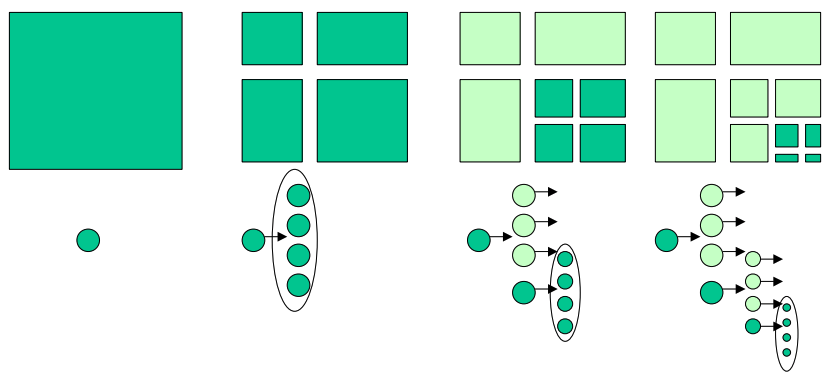
\includegraphics[width=8cm]{figuras/sting.png}
	}{
		\Fonte{\cite{Berkhin2002}}
	}
\end{figure}

O desempenho de STING depende da granularidade do nível mais baixo da estrutura de grade e o resultado dos
grupos são limitados, pois só crescem na horizontal ou vertical e sofrem para buscar grupos de formatos complexos.

Os resultados produzidos pelo STING se aproximam do agrupamento produzido pelo
DBSCAN à medida que a granularidade da estrutura de grade se aproxima de 0, podendo
também ser considerado como um método baseado em densidade, descrito a seguir.
Uma das vantagens do STING é a complexidade linear de tempo em relação ao número de objetos a serem agrupados.

\subsection{Métodos baseados em densidade}
Nesta classe de algoritmos a idéia principal é manter os grupos em crescimento, desde que sua densidade esteja acima de um certo limite. A vantagem dos algoritmos baseados em densidade, em comparação aos algoritmos de particionamento baseados em distância, é que eles podem detectar grupos de forma arbitrária. Isso também fornece uma proteção natural contra \textit{outliers}. Por outro lado, os algoritmos baseados na distância entre indivíduos detectam apenas aglomerados de forma convexa.

Os agrupamentos baseados em densidade analisam a quantidade de elementos dentro de uma vizinhança de acordo com determinados parâmetros. A ideia-chave é que, para cada instância de um grupo, a vizinhança de um determinado raio deve conter pelo menos um número mínimo de instâncias.

A possibilidade de encontrar agrupamentos de forma eventual e o fato de não precisar da definição do número de agrupamentos \cite{yip2005} como parâmetro inicial são as principais vantagens dos métodos baseados em densidade. Entretanto, alguns algoritmos podem exigir a definição de outros parâmetros, como o caso do algoritmo DBSCAN \cite{ESTER1996} abordado na próxima seção.

\subsubsection{Método DBSCAN}
\label{dbscan}
% TODO DBSCAN KDD96-037
% TODO O metodo dbscan https://www.maxwell.vrac.puc-rio.br/24787/24787_6.PDF

Este método calcula a densidade de uma região contando quantos objetos nela existem seguindo uma determinada métrica (p.ex., euclidiana ou manhattan). É um método efetivo para identificar grupos de formato arbitrário e de diferentes tamanhos, separar os ruídos dos dados, requer apenas um parâmetro de entrada, ajuda o usuário na determinação de um valor apropriado para ele e ajuda a detectar grupos e seus arranjos dentro do espaço de dados, sem qualquer informação preliminar sobre os grupos.
\cite{ESTER1996}  indicam que a noção de agrupamentos e o algoritmo DBSCAN se aplicam para espaços euclidianos de duas e três dimensões, como para qualquer espaço característico de alta dimensão. O método DBSCAN é aplicável a qualquer base de dados contendo dados de um espaço métrico, isto é, bases de dados com uma função de distância para pares de objetos. Finalmente, o DBSCAN é eficiente mesmo para grandes bancos de dados espaciais.

Para entender o método é necessário conhecer alguns conceitos básicos que são por ele utilizados: 

\begin{enumerate}
	\item Vizinhança: Determinada pela função de distância, que pode ser distância euclidiana ou distância manhattan, para dois pontos ${p}$ e ${q}$, dado por ${dist(p,q)}$.
	\item Eps: raio ao redor de um ponto. 
	\item Eps-vizinhança: a vizinhança de um ponto ${p}$ com raio Eps, dado por ${N_{Eps}(p)}$, é definido por ${N_{Eps}(p) = \big\{ q \in D | dist(p, q)  \leqslant Eps\big\} }$. Na figura \ref{fig:epsViz} abaixo os círculos representam respectivamente a vizinhança Eps dos pontos ${q}$ e ${p}$.
	\item Ponto Central: Se o Eps-vizinhança de um ponto ${p}$ contém ao menos um número mínimo, MinPts, de pontos, então o ponto ${p}$ é chamado de ponto central.
	Por exemplo, na figura \ref{fig:epsViz}, se for adotado MinPts = 4, ${p}$ é um ponto central e os demais não são pontos centrais.
	\item Ponto de Borda: Se a Eps-vizinhança de um ponto ${p}$ contém algum ponto central e menos que MinPts então o ponto ${p}$ é chamado de ponto de borda. Na figura  \ref{fig:epsViz}, ${q}$, ${r}$ e ${s}$ são pontos de borda.
	\item Diretamente alcançável: um ponto ${p}$ é alcançável se ele está no Eps-vizinhança de ${q}$ e este é um ponto central.
	\item Maximalidade: um ponto ${p}$ é alcançável se existe uma cadeia de pontos que os liga, respeitando Eps e MinPts.
	\item Conectividade: Um ponto ${p}$ está conectado a um outro ${q}$ se existe um objeto ${o}$ tal que tanto ${p}$ quanto ${q}$ são alcançáveis a partir de ${o}$, com respeito a Eps e MinPts. Logo é uma relação simétrica.
	\item Cluster: Seja D uma base de dados, um grupo C é um subconjunto não vazio de D, respeitando Eps e MinPts, onde:
		\subitem ${\forall}$ ${p}$, ${q}$ se ${q}$ ${\in}$ C e ${p}$ é alcançável a partir de ${q}$.
		\subitem ${\forall}$ ${p}$, ${q}$ ${\in}$ C ${p}$ está conectado por densidade a ${q}$.
\end{enumerate}

\begin{figure}[!ht]
	\centering
	\Caption{\label{fig:epsViz} Eps-vizinhança de ${q}$ e Eps-vizinhança de ${p}$}	
	\UECEfig{}{
		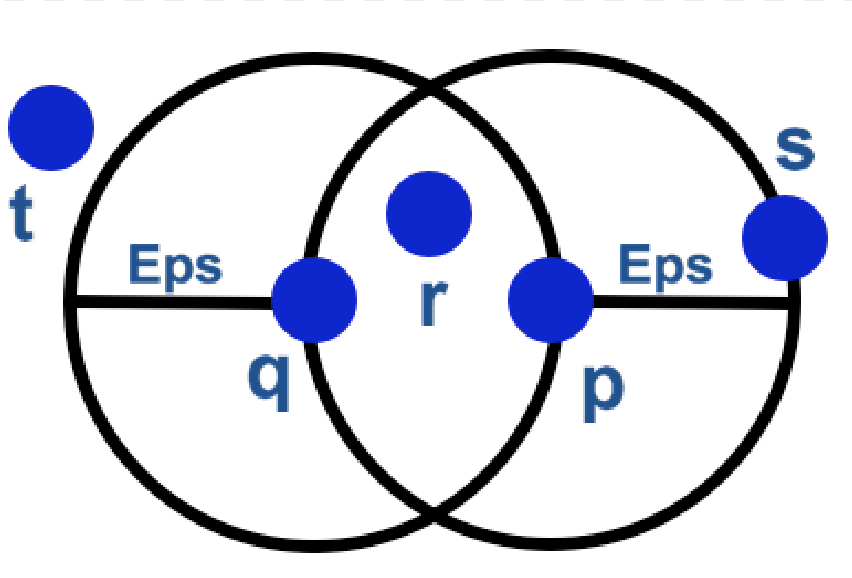
\includegraphics[width=8cm]{figuras/epsViz.png}
	}{
		\Fonte{Elaborado pelo autor}
	}
\end{figure}

O procedimento para encontrar um agrupamento é baseado no fato de que um grupo é inequivocamente determinado por qualquer de seus centros \cite{ESTER1998}. 

O DBSCAN pode utilizar a estrutura de dados R*-tree para obter um melhor desempenho, mesmo assim  a complexidade média do tempo de execução do DBSCAN será ${O (N logN)}$, onde ${N}$ é o número de objetos da base de dados, \cite{Sheikholeslami1998}.

\subsubsubsection{Algoritmo DBSCAN}

As etapas envolvidas neste algoritmo são as seguintes:

\begin{enumerate}
	\item Selecionar um ponto arbitrário ${p}$;
	\item Recuperar todos os pontos que são alcançáveis por densidade a partir do ponto ${p}$;
	\item Se ${p}$ é um ponto central, um grupo é formado;
	\item Se ${p}$ é um ponto de borda, nenhum ponto é alcançável por densidade a partir de ${p}$ e DBSCAN visita o próximo ponto do banco de dados;
	\item Continuar o processo até que todos os pontos tenham sido processados.
\end{enumerate}

% ver https://www.maxwell.vrac.puc-rio.br/24787/24787_6.PDF

\begin{algorithm}[!ht]
	\SetSpacedAlgorithm
	\caption{\label{alg:algoritmo_dbscan}Algoritmo DBScan}
	\Entrada{D, Eps1, MinPts, Delta, Epsilon}
	\Saida{C}
	\Inicio{
			\Para{i = 0 até n}{
				\Se{${o_i}$ nao foi visitado}{
					marcar ${o_i}$ como visitado\;
					Vizinhos = BuscarVizinhos(${o_i}$)\;
					\Se {|Vizinhos| < MinPts}{
						MarcarRuido(${o_i}$)\;
					}
				    \Senao{
				    	C = próximo Cluster\;
				    	adicionar ${o_i}$ ao cluster C\;
				    	expandirCluster(${o_i}$, C, Vizinhos)\;
				    }
				}
			}
	}
\end{algorithm}
\begin{algorithm}[!ht]
	\SetSpacedAlgorithm
	\caption{\label{alg:algoritmo_dbscan_exp}Algoritmo DBScan - Expandir Cluster}
	\Entrada{Vizinhos, C, MinPts}
	\Inicio{
			\Para{i = 0 até número de Vizinhos}{
				${p}$ = ${Vizinhos_{(i)}}$\;
				\Se {${p}$ ainda não foi visitado}{
					marcar ${p}$ como visitado\;
					Vizinhos2 = BuscarVizinhos(p)\;
					
					\Se {Vizinhos2 ${\geqslant}$ MinPts}{
						Vizinhos = Vizinhos ${\cup}$ Vizinhos2\;
					}
				}
				\Se{${p}$ não está em nenhum cluster}{
					adicionar ${p}$ ao cluster C\;
				}
				
			}
	}
\end{algorithm}
\pagebreak
As figuras \ref{fig:dbscanStep1}, \ref{fig:dbscanStep2} e \ref{fig:dbscanStep3} ilustram os passos da resolução do algoritmo DBSCAN.

\begin{figure}[!ht]
	\centering
	\Caption{\label{fig:dbscanStep1} DBSCAN - Identificação dos vizinhos dentro de um raio definido}	
	\UECEfig{}{
		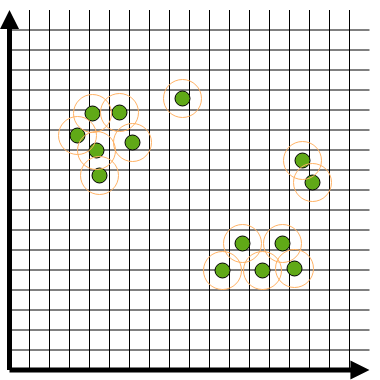
\includegraphics[width=9cm]{figuras/dbscanStep1.png}
	}{
		\Fonte{Elaborado pelo autor}
	}
\end{figure}

\begin{figure}[!ht]
	\centering
	\Caption{\label{fig:dbscanStep2} DBSCAN - Pontos que estejam dentro do raio de outro ponto estão no mesmo grupo}
	\UECEfig{}{
		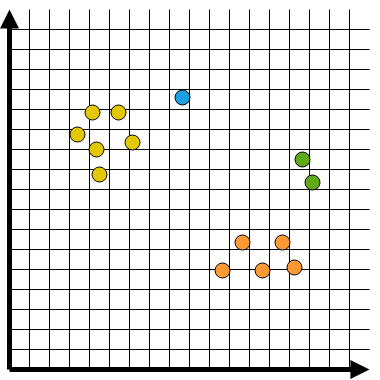
\includegraphics[width=9cm]{figuras/dbscanStep2.png}
	}{
		\Fonte{Elaborado pelo autor}
	}
\end{figure}

\begin{figure}[!ht]
	\centering
	\Caption{\label{fig:dbscanStep3} DBSCAN - Identificação dos \textit{outliers}}	
	\UECEfig{}{
		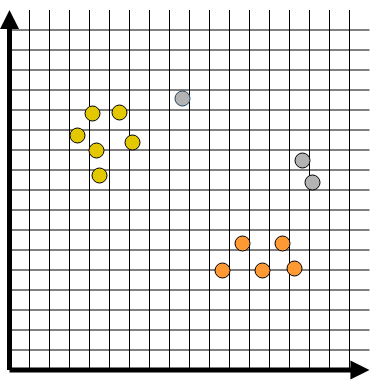
\includegraphics[width=10cm]{figuras/dbscanStep3.png}
	}{
		\Fonte{Elaborado pelo autor}
	}
\end{figure}

\subsection{Processo de detecção de \textit{outliers}}

Um \textit{outlier} é um objeto que desvia de um padrão do conjunto de dados ao qual ele pertence. Segundo \cite{Barnett1978Outliers}, é uma observação (ou um conjunto de observações) que parece ser inconsistente com o restante daquele conjunto de dados. Ele descreve as causas de ocorrência de \textit{outliers} como: são objetos que pertencem a população; erro de medição na coleta de dados; erros de execução ao adquirir dados de amostragem de mais de uma população.

Em processos de agrupamento é muito importante a detecção dos \textit{outliers}, uma vez que estes objetos podem deturpar o processo de classificação de forma muito danosa. Deve-se pois considerar também que vários dos métodos de agrupamentos naturais servem também como bons detectores de \textit{outliers}, no entanto as características destes indivíduos podem ser muito relevantes para a separação completa dos demais que têm similaridades características de cada um dos grupos a que pertencem.

%Outlier x Ruídos
Uma questão a se considerar é a diferença entre o significado de \textit{outlier} e ruído. Enquanto ruído refere-se à modificação de valores originais, os \textit{outliers} contêm informações importantes para a descricão do conjunto de dados \cite{chandola2009}. Ruído é uma anomalia indesejada no dado causada por imprecisão nos atributos de entrada, erro ao rotular os dados ou até por atributos de dados que foram excluídos, mas afetam a rotulação \cite{alpaydin2010}.

A detecção de \textit{outliers} refere-se ao problema de encontrar padrões que exibem um comportamento diferenciado em relação à maioria dos dados \cite{chandola2009}. Caracterizar o processo de detecção de ruídos e \textit{outliers} é muito importante, pois permite a redução de prejuízos e uma melhor análise dos dados. As técnicas de detecção \textit{outlier} têm sido aplicadas a um grande número de aplicações tais como: detecção de fraudes, processamento de imagens, detecção de intrusão, medicina e detecção de dados rotulados incorretamente.

\subsubsection{Técnicas de detecção de \textit{outliers}}
As técnicas de detecção de \textit{outliers} podem ser aplicadas em detecção de padrões raros, remoção de ruídos, detecção de padrões ainda não observados, etc. Deve-se considerar a complexidade computacional dada a grandes quantidades de dados disponíveis para manipulação. Alguns fatores são importantes para classificar as técnicas de detecção de \textit{outliers}: a natureza dos dados, o tipo de \textit{outlier}, a disponibilidade dos rótulos, a utilização de parâmetros, a manipulação de grande volume de dados, etc. A seguir, algumas das técnicas de detecção de \textit{outliers}.

\subsubsubsection{Técnicas estatísticas}
As técnicas estatísticas desenvolvem um modelo estatístico (geralmente para um comportamento normal) aos dados fornecidos e, em seguida, aplicam um teste de inferência estatística para determinar se um determinado dado pertence ou não a esse modelo. Dados com baixa probabilidade de pertencerem ao modelo estatístico são declaradas como \textit{outlier} \cite{chandola2009}.

\subsubsubsection{Técnicas baseadas em distância}
Técnicas baseadas em distância são aquelas que variam a forma de computar a distância de um objeto em relação aos vizinhos mais próximos. A distância pode ser medida por meio da distância de Manhattan ou Euclidiana e a escolha do valor não depende do conjunto de dados. Existem técnicas que se baseiam no cálculo da densidade de objetos para identificar \textit{outliers}. O funcionamento segue duas etapas: para cada dado a vizinhança é computada usando uma medida de distância ou de similaridade entre dois dados. Na segunda etapa, os vizinhos são analisados para determinar se o dado é normal ou \textit{outlier}.

\subsubsubsection{Técnicas baseadas em agrupamento de dados}
Técnicas baseadas em agrupamento levam em consideração que dados normais pertencem a grupos grandes e densos, enquanto objetos de dados \textit{outliers} não se enquadram em nenhum grupo. O principal objetivo dos algoritmos de agrupamento de dados é na identificação de grupos, e por isso é necessário estabelecer algum critério para diferenciar um dado normal de um \textit{outlier}.

O algoritmo de BIRCH \cite{Zhang1996} mencionado na seção \ref{sub:birch}, considera como \textit{outliers} as entradas de baixa densidade presentes nos nós folhas da AC-árvore.

Estas técnicas podem ser divididas em semi-supervisionadas e não-supervisionadas. As técnicas semi-supervisionadas normalmente usam dados normais para gerar grupos que representam o comportamento normal dos dados, um objeto novo de teste é alocado a um grupo, se não estiver próximo de nenhum é categorizado como \textit{outlier}. Já as técnicas não-supervisionadas usam um algoritmo conhecido de agrupamento para agrupar os dados e analisam cada instância com relação aos grupos formados.

\section{Agrupamentos Dinâmicos}
Um agrupamento dinâmico é definido como sendo um conjunto de indivíduos de alta similaridade que se mantêm unido ao longo do tempo, caracterizado por um certo número de indivíduos que mantêm a identidade do grupo. O processo de classificação de agrupamentos dinâmicos é a metodologia que identifica tais grupos que se constroem e se desfazem no tempo, tal metodologia identifica classes naturais e ao mesmo tempo as relaciona a outras classes em similaridade que ocorrem antes e depois delas no tempo. Tal relação precisa ser bem estabelecida e consistente para que se perceba os movimentos evolutivos no tempo.

Várias formas diferentes de tipos de dados espaço-temporais estão disponíveis em aplicativos reais. Embora todos compartilhem a disponibilidade de algum tipo de aspecto espacial e temporal, a extensão dessas informações e a maneira como elas são relacionadas podem se combinar com vários tipos diferentes de objetos de dados \cite{maimon:2005}. Com base em duas dimensões, é dada uma possível classificação destes tipos de dados:

\begin{itemize}
	\item a dimensão temporal descreve em que medida a evolução do objeto é capturada pelos dados. O caso mais básico consiste em objetos que não evoluem, onde apenas um \textit{snapshot} estático de cada objeto está disponível. Em contextos um pouco mais complexos, cada objeto pode alterar seu status, mas apenas seu valor mais recente é conhecido (um \textit{snapshot} atualizado), portanto, sem qualquer conhecimento sobre seu histórico passado. No caso extremo é onde o histórico completo do objeto é mantido, formando assim uma série temporal do status que ele percorreu;

	\item a dimensão espacial descreve se os objetos considerados estão associados a um local fixo (por exemplo, as informações coletadas por sensores fixados no solo) ou podem se mover, ou seja, sua localização é dinâmica e pode mudar no tempo.
\end{itemize}

\subsection{Método ST-DBSCAN}
\label{stdbscan}

% Comentar um bloco de código: \iffalse \fi
Para agrupar os pontos levando em conta o fator tempo é necessário uma alteração no algoritmo DBSCAN \cite{ESTER1998}, e com isso detectar os grupos em relação ao tempo. Esse algoritmo usa apenas um parâmetro de distância Eps para medir a similaridade de dados espaciais com uma dimensão. A fim de suportar dados espaciais bidimensionais, o ST-DBSCAN \cite{Birant2007STDBSCANAA} usa duas métricas de distância, Eps1 e Eps2, para definir a similaridade por uma conjunção de dois testes de densidade.
O algoritmo ST-DBSCAN é construído modificando o algoritmo DBSCAN. Em contraste com o algoritmo de agrupamento baseado em densidade existente, o algoritmo ST-DBSCAN tem a capacidade de descobrir agrupamentos de acordo com valores não espaciais, espaciais e temporais dos objetos. As três modificações feitas no algoritmo DBSCAN são as seguintes:
\begin{itemize}
\item Permitir o algoritmo ST-DBSCAN descobrir grupos em dados espaciais-temporais.
\item Introdução do fator de densidade atribuído a cada grupo, que é o seu grau de densidade, para encontrar objetos de ruído quando existem grupos de diferentes densidades.
\item A terceira modificação fornece uma comparação do valor médio de um grupo com o novo valor resultante. Necessária para resolver os conflitos em pontos de borda.
\end{itemize}

O algoritmo DBSCAN não é satisfatório quando existem agrupamentos de diferentes densidades. Para superar esse problema,  o ST-DBSCAN atribui a cada grupo um fator de densidade, que é o grau da densidade do grupo.
A função DensityDistance é dada por:

${DensityDistance = \frac{DensityDistanceMax}{DensityDistanceMin}}$
\linebreak
onde DensityDistanceMax de um objeto ${p}$ denota a distância máxima entre o objeto ${p}$ e seus vizinhos dentro do raio Eps. Da mesma forma, DensityDistanceMin de um objeto ${p}$ denota a distância mínima entre o objeto ${p}$ e seus vizinhos dentro do raio Eps.

${DensityDistanceMax(p) = max\big\{ dist(p, q) | q \in D \wedge dist(p, q)  \leqslant Eps\big\} }$

${DensityDistanceMin(p) = min\big\{ dist(p, q) | q \in D \wedge dist(p, q)  \leqslant Eps\big\} }$
\linebreak

O fator de densidade de um grupo ${C}$ é dado por:

${DensityFactor(C) = 1\big/\left [   \frac{\sum_{p\in C}DensityDistance(p)}{|C|} \right ]}$
\linebreak

Com esse fator é possível evitar problemas de agrupamentos com grande variação de densidade, onde os grupos são pequenos e muito densos ou grandes e pouco densos.

\subsubsection{Algoritmo ST-DBSCAN}
Uma grande diferença entre o DBSCAN e o ST-DBSCAN é a utilização de um segundo parâmetro EPS, onde é usado para medir a similaridade de valores não espaciais. Nesta pesquisa usa-se o tempo como EPS de valor não espacial. Para dois pontos serem considerados vizinhos eles devem respeitar os limites de espaço e tempo parametrizados por EPS1 e EPS2 \cite{Birant2007STDBSCANAA}.

\begin{enumerate}
	\item O algoritmo começa com o primeiro ponto ${p}$ no banco de dados D.
	\item Este ponto ${p}$ é processado de acordo com o algoritmo DBSCAN e o próximo ponto é tomado.
	\item A função BuscarVizinhos(p, Ep1, Ep2) recupera todos os pontos que tem uma distância menor que Eps1 e Eps2 para o ponto ${p}$. Se os pontos recuperados não podem ser alcançados o ponto é atribuído como ruído, onde o ponto selecionado não tem vizinhos suficientes para ser armazenado em grupo.
	\item Os pontos marcados como ruído podem ser alterados posteriormente, se não forem diretamente alcançáveis pela densidade, mas eles são alcançáveis por densidade de algum outro ponto do banco de dados. Isso acontece para pontos de borda de um grupo.
	\item Se o ponto selecionado tiver vizinhos suficientes dentro das distâncias Eps1 e Eps2 - se for um ponto central, então um novo grupo será construído.
	\item Todos os vizinhos diretamente atingíveis por densidade desse ponto central também são incluídos.
	\item O algoritmo reúne iterativamente pontos acessíveis por densidade a partir desse ponto central usando uma pilha.
	\item Se o objeto não estiver marcado como ruído ou não estiver em um grupo e a diferença entre o valor médio do grupo e o novo valor é menor do que o valor limite para incluir em um grupo, ${\Delta E}$, ele é colocado no grupo atual.
	\item Se dois grupos ${C_1}$ e ${C_2}$ estão muito próximos um do outro, um ponto ${p}$ pode pertencer a ambos ${C_1}$ e ${C_2}$. Então o ponto ${p}$ é atribuído ao grupo que foi descoberto primeiro.
	\item Depois de processar o ponto selecionado, o algoritmo seleciona o próximo ponto em D e o algoritmo continua iterativamente até que todos os pontos tenham sido processados.
\end{enumerate}

\pagebreak
\begin{algorithm}[!ht]
	\SetSpacedAlgorithm
	\caption{\label{alg:algoritmo_stdbscan}Algoritmo ST-DBScan}
	\Entrada{D, Eps1, Eps2, MinPts, ${\Delta E}$}
	\Saida{C = (${C_1}$, ${C_2}$, ... ${C_k}$) Conjunto de clusters}
	\Inicio{
		\Para{i = 1 até n}{
			\Se {${o_i}$ não está no cluster}{
				Vizinhos = BuscarVizinhos(${o_i}$, Eps1, Eps2)\;
				\Se {|Vizinhos| < MinPts}{
					marcar ${p}$ como ruído\;
				}
			   \Senao{
			   		\Para{j = 1 até |Vizinhos|}{
			   			RotularPontos(${X_j}$)\;
			   			AdicionarPontosAoCluster(${X_j}$, ${C_i}$)\;
			   		}
		   		\Enqto{existir pontos na vizinhança de ${o_i}$}{
		   			pontoAtual = vizinho(${o_i}$)\;
		   			Vizinhos2 = BuscarVizinhos(pontoAtual, Eps1, Eps2)\;
		   			\Se{|Vizinhos2| >= MinPts}{
		   				\Para{ todo ${o_y}$}{
		   					\Se{(${\neg}$ehRuido(${o_y}$) ${\vee}$ ${\neg}$estaNumGrupo(${o_y}$)) ${\wedge}$ DensidadeMediaDoGrupo($C_i$) +${o_y}$ > ${\Delta E}$ }{
		   						AdicionarPontosAoCluster(${o_y}$, ${C_i}$)\;
		   					}
		   				}
		   			}
		   		}
		       }
			}
		}
	}
\end{algorithm}

Um exemplo do ST-DBSCAN é apresentado em \cite{st-twitter}, onde o Eps1 é definido como 70km, 85km e 100km, e MinPts como 5, 10 e 15. Já o Eps2 como 2 dias. Os resultados para os 9 conjuntos de parâmetros são mostrados na figura \ref{fig:st-twitter}, revelando claramente que um maior Eps e um menor MinPts correspondem a maiores grupos espaço-temporais. Na Figura \ref{fig:st-twitter}(a), duas regiões espaço-temporais são representadas por duas elipses pretas, denominadas STR1 e STR2.
Os parâmetros de cada conjunto são:
(a) Eps = 70, MinPts = 5; (b) Eps = 85, MinPts = 5; (c) Eps = 100, MinPts = 5; (d) Eps = 70, MinPts = 10; (e) Eps = 85, MinPts = 10; (f) Eps = 100, MinPts = 10; (g) Eps = 70, MinPts = 15; (h) Eps = 85, MinPts = 15; (i) Eps = 100, MinPts = 15. O Eps2 (2 dias) é o mesmo para todos os conjuntos.

\begin{figure}[!ht]
	\centering
	\Caption{\label{fig:st-twitter} ST-DBSCAN - Os clusters espaço-temporais descobertos}
	\UECEfig{}{
		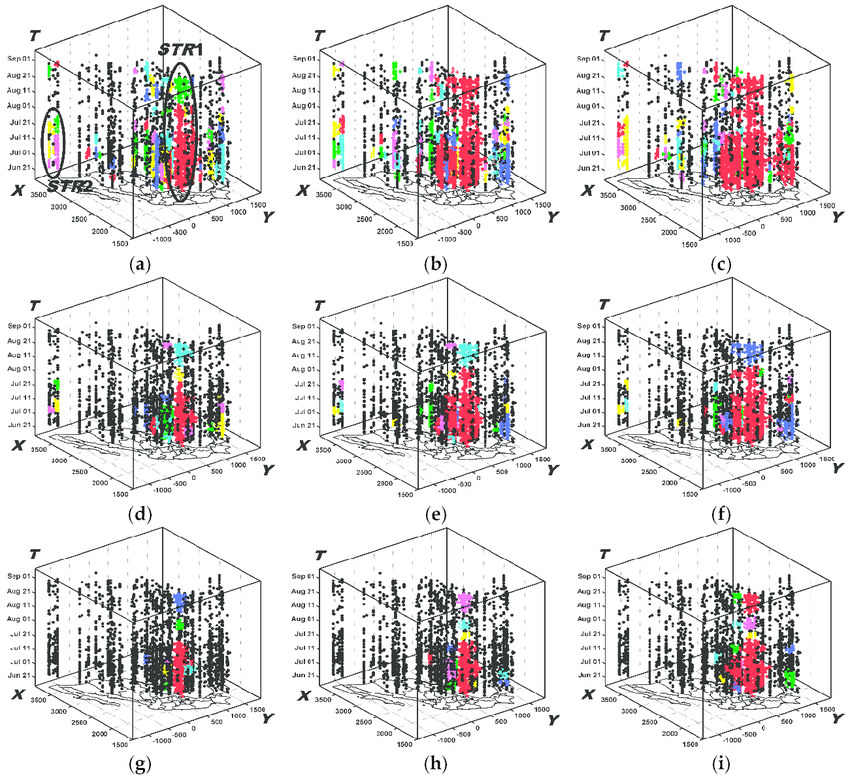
\includegraphics[width=16cm]{figuras/st-twitter.png}
	}{
		\Fonte{\cite{st-twitter}}
	}
\end{figure}

\subsection{Método ST-IGN}
\label{stign}
O método IGN dinâmico consiste da aplicação do método IGN estático \cite{simposioNeg2003} sobre cada uma das $n$ instâncias (estados) geradas a partir de um período (intervalo fixo de estados) definido pelo processo de identificação da dinâmica do comportamento dos objetos. O método rotula os grupos naturais encontrados na unidade de tempo $i$ com base na máxima densidade de objetos que se mantém no mesmo grupo após uma divisão e/ou aglomeração.

A seguir são listados os elementos e parâmetros necessários para aplicação do método:
\begin{itemize}
\item Objetos de Entrada definidos por estado;
\item Unidade de tempo estático (uma fotografia);
\item Período Dinâmico (intervalo interno da fotografia);
\item Ganho Estático (possibilidade de ganho de estados em períodos distintos).
\end{itemize}

Os indivíduos podem ser representados atráves de uma entrada de dados, que consiste de uma tabela com as seguintes características:

\begin{table}[!ht]
	\centering
	\Caption{\label{tab:label_da_tabela} IGN Dinâmico - Estrada de dados}
	\UECEtab{}{
		\begin{tabular}{c c c c c c c c}
			\toprule
	            & ${X_1}$ & ${X_2}$ & ${X_3}$ & ... & ${X_p}$ & ${X_t}$ &\\
	    	    ${I_{11}}$	&  &  &  &  &  &  & 1\\
	    	    ${I_{21}}$	&  &  &  &  &  &  & 1\\
	    	    . &  &  &  &  &  &  & .\\
	    	    . &  &  &  &  &  &  & .\\
	    	    . &  &  &  &  &  &  & .\\
	    	    ${I_{n1}}$	&  &  &  &  &  &  & 1\\
	    	    ${I_{12}}$	&  &  &  &  &  &  & 2\\
	    	    . &  &  &  &  &  &  & .\\
	    	    . &  &  &  &  &  &  & .\\
	    	    . &  &  &  &  &  &  & .\\
	    	    ${I_{n2}}$	&  &  &  &  &  &  & 2\\
	    	    ${I_{1m}}$	&  &  &  &  &  &  & m\\
	    	    . &  &  &  &  &  &  & .\\
	    	    . &  &  &  &  &  &  & .\\
	    	    . &  &  &  &  &  &  & .\\
	    	    ${I_{nm}}$	&  &  &  &  &  &  & m\\
			\bottomrule
		\end{tabular}
	}{
		\Fonte{Elaborado pelo autor}
    }
\end{table}

Onde, 

${I_{ik}}$, é o indivíduo do estado \textit{k};

${X_s}$, é o valor do atributo referente a variável \textit{s};

${X_t}$, é a variável que indica o estado \textit{t} a que pertence o indivíduo.

Sejam estão os seguintes parâmetros para avaliação de um movimento dinâmico:
\begin{itemize}
    \item NE - Número de estados;
    \item TPE - Tamanho do período estático. Quantidade de estados sequenciais a serem tomados, ${TPE \geqslant 1}$;
    \item TPD - Tamanho do período dinâmico. Toma os próximos TPE estados e elimina os TPE estados anteriores, ${TPD \geqslant 1}$;
    \item GD - Ganho dinâmico. Quantidade de estados ganhos ou perdidos entre dois períodos dinâmicos subsequentes, ${GD \geqslant 0}$;
    \item GN[k] - É o conjunto dos grupos naturais formados na iteração \textit{k};
    \item DATA[k] - É o conjunto formado pelos dados do período estático \textit{k}.
\end{itemize}

O algoritmo que define o método IGN Dinâmico pode ser escrito da seguinte forma:

\begin{algorithm}[!ht]
	\SetSpacedAlgorithm
	\caption{\label{alg:algoritmo_stign}Algoritmo ST-IGN}
	\Entrada{TPE, TPD, GD}
	\Saida{GN - Grupos Naturais}
	\Inicio{
	    i = TPE\;
	    k = 1\;
	    s = 0\;
	    \Enqto{${s \geqslant NE}$}{
    	    \Se {${s = 0}$} {
	            ${t_1 = 1}$\;
    	    }
    	    \Senao {
    	        ${t_1 = t_1 + TPD}$\;
    	    }
    	    ${t_2 = t_1 + TPE + GD - 1}$\;
    	    ${DATA[k] = \{ I_s, s = t_1, ..., t_2 \} }$\;
    	    IGN-Estatico(${DATA[k], GN[k]}$)\;
    	    AvaliarRotular(${GN[k]}$, ${GN[[k-1]}$)\;
    	    ${k = k + 1}$\;
	    }
	}
\end{algorithm}

O procedimento IGN-Estático retorna o agrupamento ${GN[k]}$ para os dados do período estático ${DATA[k]}$. Já o algoritmo AvaliarRotular, refaz a rotulação e caracterização do grupo ${GN[k]}$ com base na rotulação do agrupamento anterior ${GN[k - 1]}$, preservando ao máximo os elementos deste agrupamento no novo agrupamento.

A figura \ref{fig:ign_avaliar_rotular} apresenta o processo de rotulação do procedimento AvaliarRotular, para os grupos formados para dados do período ${k - 1}$ e \textit{k}. Sendo ${GN[k]}$ e ${GN[k - 1]}$, onde ${GN[k] \cap GN[k - 1] \neq \varnothing 
}$, a rotulação de ${GN[k - 1]}$ será mantida em ${GN[k]}$ naqueles grupos que têm a maior quantidade de elementos em relação ao seu gerador em ${GN[k - 1]}$. Caso não haja interseções entre grupos nos períodos subsequentes distintos, novos rótulos serão atribuídos a estes grupos.

\begin{figure}[!ht]
	\centering
	\Caption{\label{fig:ign_avaliar_rotular} Procedimento AvaliarRotular e evolução do IGN-Dinâmico para 3 períodos estáticos}	
	\UECEfig{}{
		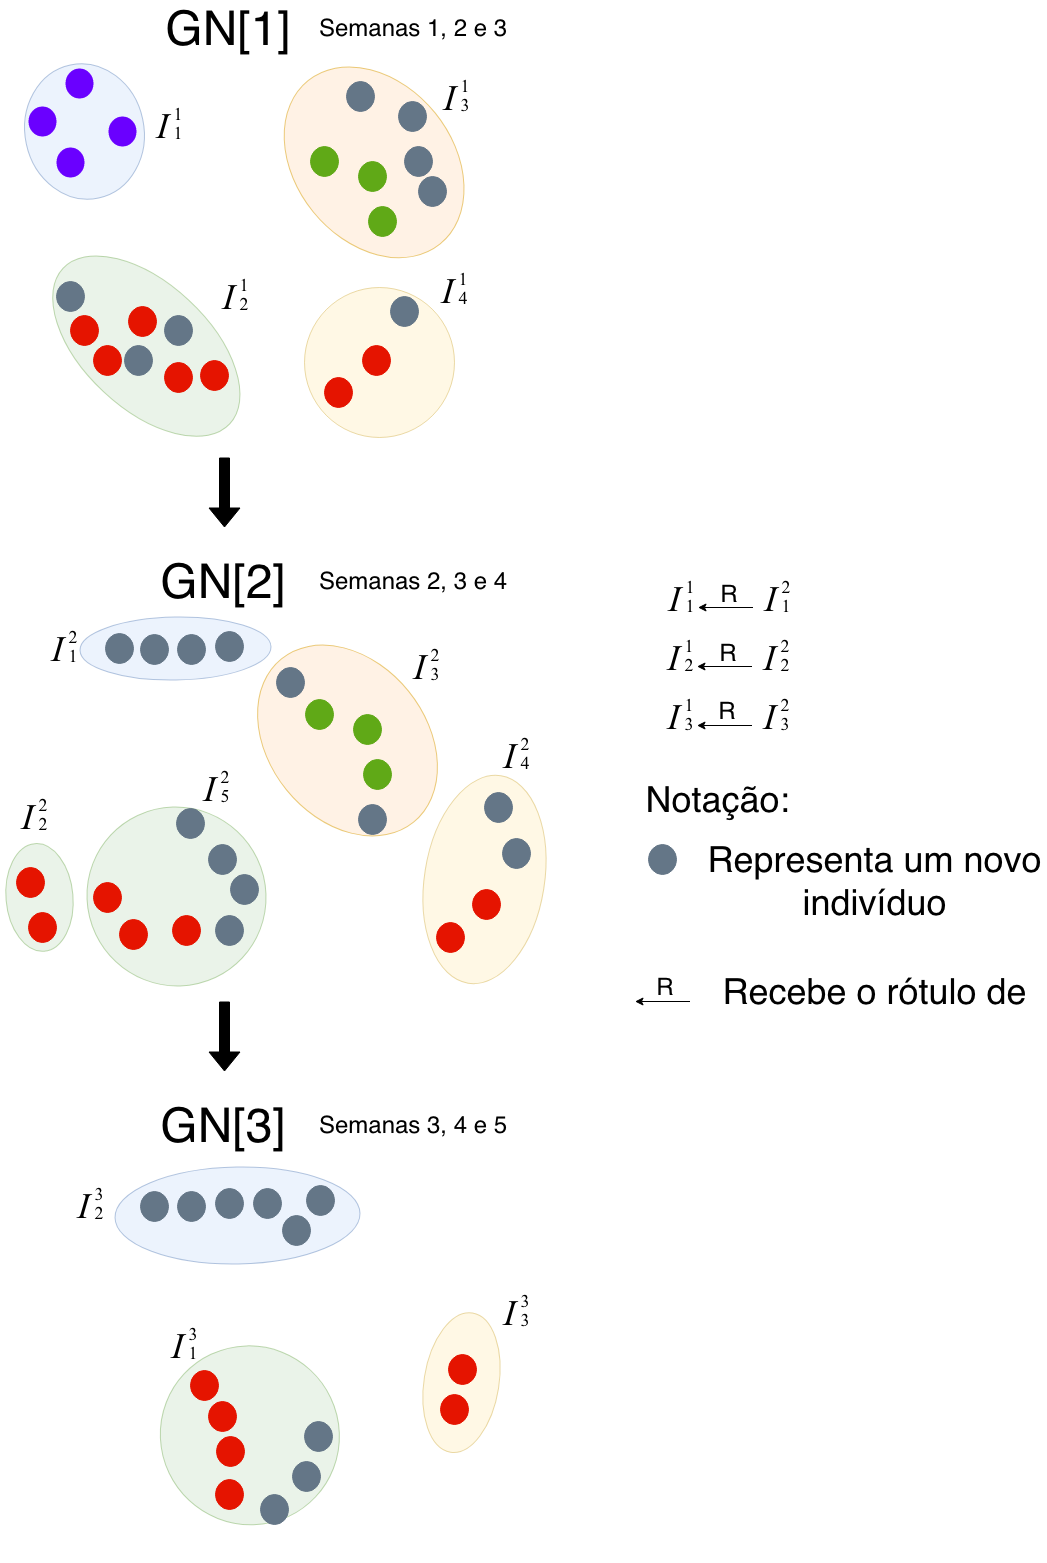
\includegraphics[width=14cm]{figuras/GN.png}
	}{
		\Fonte{Elaborado pelo autor}
	}
\end{figure}

Este procedimento foi elaborado por \cite{webdengue2008}, cujo principal objetivo era de mapear a evolução da dengue na cidade de Fortaleza, tomando como base as características de evolução dos casos e focos da doença observados em 2005 para a Regional II de Fortaleza-CE. A pesquisa se preocupou em definir intervalos de observação que justificassem um comportamento de evolução do mosquito Aedes aegypt (Focos) e dos casos humanos da doença, utilizando como ferramenta principal o algoritmo estático IGN e o \textit{framework} WebDengue \cite{webdengue2008}. Este framework é uma solução de vigilância epidemiológica composta por um conjunto de sistemas computacionais. Essas tecnologias combinam geoprocessamento, sistemas de apoio a decisão, sistemas de bancos de dados e a aquisição de dados remotos, como mostrado na figura \ref{fig:webdengue} \cite{webdengue2008}.

\begin{figure}[!ht]
	\centering
	\Caption{\label{fig:webdengue} Estrutura computacional proposta para a gestão da dengue}	
	\UECEfig{}{
		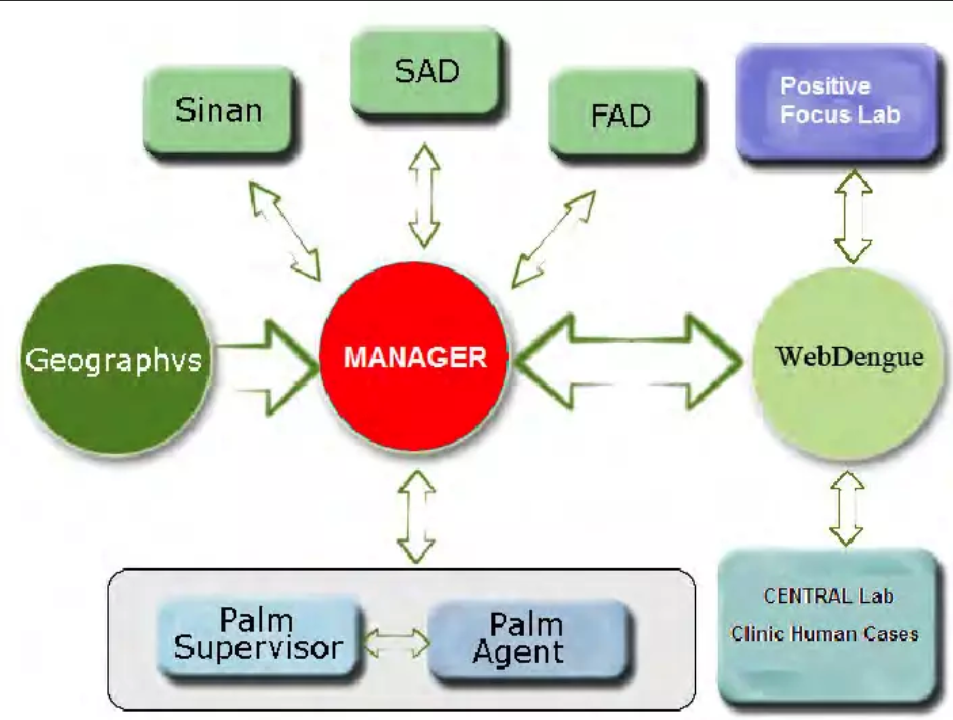
\includegraphics[width=12cm]{figuras/webdengue.png}
	}{
		\Fonte{Sistema WebDengue \cite{webdengue2011} }
	}
\end{figure}

Os dados foram tomados a partir dos informes diários de casos e focos, onde um estado é definido como o período de uma semana. Do conjunto de observações se consideram seis ternos de semana (1-2-3, 2-3-4, 3-4-5, 4-5-6) de Abril/2005 a Maio/2005 para o comportamento dos focos. Os casos são tomados para o final de cada período em razão de serem eles consequentes de possível infestação pela picada do mosquito Aedes aegypti, tomou-se então quatro quinzenas (3-4, 4-5, 5-6, 6-7) de Maio/2005 a Junho/2005 para avaliar este comportamento.

\pagebreak

\subsection{Detecção de \textit{outliers} espaço-temporais}
\textit{Outliers} são tradicionalmente definidos como instâncias que são notavelmente diferentes da maioria das instâncias no conjunto de dados. Em aplicações espaço-temporais, detectar \textit{outliers} ajuda a identificar fenômenos interessantes, mas raros, por exemplo, uma trajetória irregular tomada por um veículo de táxi ou a mudança das frequências de inundações e secas em determinadas áreas devido a mudanças climáticas ou ações humanas que mudam a ecologia de uma região \cite{Atluri:2018}.

Um aspecto a considerar por trás da detecção de \textit{outliers} espaço-temporais é que isso reflete na descontinuidade em atributos não espaço-temporais dentro de uma vizinhança espaço-temporal \cite{cheng:2014}.

Alguns estudos descobrem \textit{outliers} considerando somente seus vizinhos temporais, enquanto outros trabalhos dizem respeito a \textit{outliers} apenas em relação a seus vizinhos espaciais. Combinando essas duas noções, um \textit{outlier} espaço-temporal (ST-Outlier) é um objeto espaço-temporal cujos atributos não-espaciais e não-temporais são significativamente diferentes dos atributos dos outros objetos em suas vizinhanças espaciais e temporais \cite{gupta:2014}.

\cite{Birant2006SpatiotemporalOD} propuseram um mecanismo de detecção ST-Outlier baseado em densidade com 3 passos:
\begin{enumerate}
    \item Agrupar usando um DBSCAN modificado. Para suportar o aspecto temporal, uma árvore é percorrida para encontrar
os vizinhos temporais de qualquer objeto dentro de um determinado raio. Para encontrar valores discrepantes quando os grupos têm diferentes densidades, o algoritmo atribui um fator de densidade a cada grupo e compara o valor médio de um grupo com o novo valor de entrada;
    \item Verificar os vizinhos espaciais para saber se esses possíveis \textit{outliers} também são \textit{outliers} espaciais;
    \item Verificar os vizinhos temporais dos \textit{outliers} espaciais.
\end{enumerate}

	\section{Redes dinâmicas}
 \label{chap:redes-dinamicas}
 % Clustering Dynamic Spatio-Temporal Patterns in the Presence of Noise and Missing Data: https://www.ijcai.org/Proceedings/15/Papers/365.pdf
 %TODO --- Introduzir o processo de previsão de agrupamentos espaço temporais ---
 
Para redes dinâmicas, o foco é tipicamente em uma classe de redes e questões referentes às estrutura dessa classe de rede, como a estrutura evoluiu e como isso afeta sistemas dinâmicos na rede. As redes temporais normalmente são mais orientadas a dados - onde se investiga um conjunto de dados, suas estruturas e como, por exemplo, surtos epidêmicos se comportariam sobre ele \cite{holme:colloquium}.

Uma observação sobre endemias é que casos e focos destes tendem a estar mais próximos do que distantes no espaço e no tempo. Por exemplo, o casos de dengue de amanhã tem mais probabilidade de serem semelhantes aos casos de hoje do que de um mês atrás ou mais. Da mesma forma, os casos num raio de 300 metros tendem a ser mais semelhantes do que os casos a 10 quilômetros ou mais de distância. Estas observações são referidas como dependência temporal e espacial.

\subsection{Previsão e Predição Espaço-Temporal}

A aceitação de modelos espaço-temporais tem sido tradicionalmente limitada pela escassez de conjuntos de dados espaço-temporais em grande escala \cite{Griffith2010}. Essa situação foi revertida nas últimas décadas e com grande quantidade de dados exige-se métodos rápidos e eficazes para lidar com eles. Os modelos espaço-temporais podem ser divididos em duas categorias: métodos estatísticos ou paramétricos e métodos de aprendizagem de máquina ou não-paramétricos.


\subsection{Agrupamento de dados baseado em predição}

A tarefa de predição visa descobrir o valor futuro de um determinado atributo de dados. É uma área com variedade de aplicações em diversas campos do conhecimento como meteorologia e detecção de doenças. Por exemplo, um médico gostaria de prever a reação de seus pacientes a um novo medicamento para diabetes, particularmente a duração dos episódios de hipoglicemia.

Na previsão de eventos, é desejável prever a ocorrência de um evento ou o número de ocorrências de um evento ou a duração de um evento, dada a existência de certas condições. Por exemplo, um médico acaba de colocar um de seus pacientes epilépticos em uma nova droga que é muito eficaz, mas após o início da terapia pode causar um grave ataque de enxaqueca. O médico gostaria de prever a duração desse ataque, considerando o conhecimento sobre a idade do paciente e o número e duração dos ataques epilépticos no último ano. Nos problemas de previsão de eventos que lidam com a previsão da duração de um evento pode ser modelada usando uma variável contínua e pode-se usar a regressão linear para sua previsão, onde a regressão linear é um dos métodos de regressão mais amplamente disponíveis \cite{Mitsa:2010}.

Na previsão de séries temporais, os dados são informações históricas obtidas em intervalos de tempo regulares. Informações sobre padrões passados podem ser usadas para prever padrões futuros. No exemplo da enxaqueca, os dados poderiam ser a duração dos ataques de enxaqueca de outros pacientes sobre a droga, juntamente com informações sobre suas idades, condições médicas preexistentes e gravidade da epilepsia.

\subsection{Método de Lahiri}
\label{lahiri}
\cite{lahiri2007} apresentam um algoritmo de predição em redes temporais, e que usa a ideia de que certas interações sinalizam a ocorrência de outros em algum momento no futuro. Através de análises estatísticas o algoritmo mede o atraso entre as interações, e com isso pode-se prever quando certas interações vão ocorrer com base em observações passadas e atuais. Propõe-se a utilização de subgrafos frequentes e discute como identificar subgrafos que persistem em redes temporais.

\cite{lahiri2008} em seguida propõe um novo problema de mineração de dados para redes dinâmicas: detecção de todos os padrões de interação que ocorrem em intervalos de tempo regulares.

\subsection{O modelo Dynagraph}

A representação dos dados de indivíduos no espaço-tempo é muito importante, para que também se possa acompanhar a solução obtida pelos métodos de agrupamento estudados. O Dynagraph \cite{dynagraph} é um modelo computacional que permite, a partir de uma estrutura de dados simples, modelo de um Grafo ou Rede Dinâmica, representar com o mínimo custo de armazenamento a evolução de uma instância de observação e estudos. Ele acompanha a evolução dos conjuntos de um grafo: de nós e ligações (arcos e elos), como inserção/retirada ao longo do tempo, e mudança de suas características (posição, cor, forma, tamanho, e outras), por meio de um Editor de Características.

Trata-se de um poderoso instrumento de visualização e representação de eventos discretos espaço-temporais em mapas geográficos bidimensionais, que permite incorporar recursos de agrupamentos, predições e previsões de eventos que são discretizados numa determinada medida de intervalos temporais (segundos, minutos, horas, dias, semanas, decêndios, quinzenas, meses, anos).

\subsubsection{Estrutura de Dados}

A estrutura de dados usada no Dynagraph segue a notação de Objeto Javascript (JSON), que é um formato de texto de intercâmbio de dados \cite{douglas}. A figura \ref{fig:jsondynagraph} mostra como é essa estrutura seguindo três objetos principais: ``metadata'', ``binding'' e ``data''.

Em ``metadata'' são definidos os campos para utilização de qualquer identificador, por exemplo: é possível utilizar ``ini'' e ``fim'',
que representam o tempo inicial e final de um elemento, no lugar de ``start'' e ``end'' respectivamente.

Na figura \ref{fig:jsondynagraph}, em ``binding'' são definidas as características dos vértices e arestas.

Seguindo o exemplo da mesma figura, ``vertex'' poderá
ser do tipo ``v1'', ``v2'' e ``v3'', onde cada tipo contém informações da forma do vértice. Essa forma pode ser uma imagem no formato
``png'' ou ``jpg'' ou customizada com as seguintes características:
\begin{itemize}
\item path: círculo ou seta;
\item fillColor: cor do preenchimento;
\item strokeColor: cor da borda;
\item fillOpacity: opacidade;
\item scale: tamanho;
\item strokeWeight: espessura da borda.
\end{itemize}

A aresta, ou ``polyline'', segue uma estrutura semelhante à do ``vertex'', porém com algumas particularidades como repetição de um símbolo
ao longo da aresta, e uma customização no campo ``path'' seguindo a notação SVG\footnote{\label{note} Scalable Vector Graphics - é uma forma de descrever de forma vetorial desenhos e gráficos bidimensionais}.

Em ``data'' são definidos os elementos do grafo, os tempos de início e fim de cada elemento ou tempo de existência. No caso dos vértices, a posição de cada elemento pode ser escrita no formato UTM ou latitude e longitude.
O tipo de cada elemento, descrito em ``binding'', e no caso das arestas, são definidos os pontos de origem e destino.

Na figura \ref{fig:jsondynagraph} vemos a estrutura de construção de um grafo dinâmico. Os campos ``metadata'' e ``binding'' foram omitidos para evidenciar o objeto ``data''.
\FloatBarrier
\lstinputlisting[language=Java, basicstyle=\tiny]{figuras/new.json}
\begin{figure}[htbp]
  \caption{Estrutura JSON usada pelo Dynagraph}
  \label{fig:jsondynagraph}
\end{figure}


\subsubsection{Editor de Características}

O Editor de Características é uma extensão do software Dynagraph. Ele permite alterar os atributos visuais dos vértices e aresta de um grafo dinâmico. Com ele pode-se criar novos tipos de dados e com isso diferenciar, por exemplo, focos de casos de dengue e tipos de dengue.
Essa extensão permite criar com os seguintes atributos: Rótulo, Opacidade, Escala, Espessura da Borda, Cor da Borda e Cor de Preenchimento. Outra opção é utilizar uma imagem.
 
A figura \ref{fig:edCaMenu} exibe a localização do Editor de Características na aplicação em um menu lateral com as seguinte opções: Vértice, Aresta e um painel, este exibe a data atual e número de vértices e arestas em análise.
\begin{figure}[!ht]
	\centering	
	\caption{\label{fig:edCaMenu} Editor de Características: menu lateral}
	\UECEfig{}{
		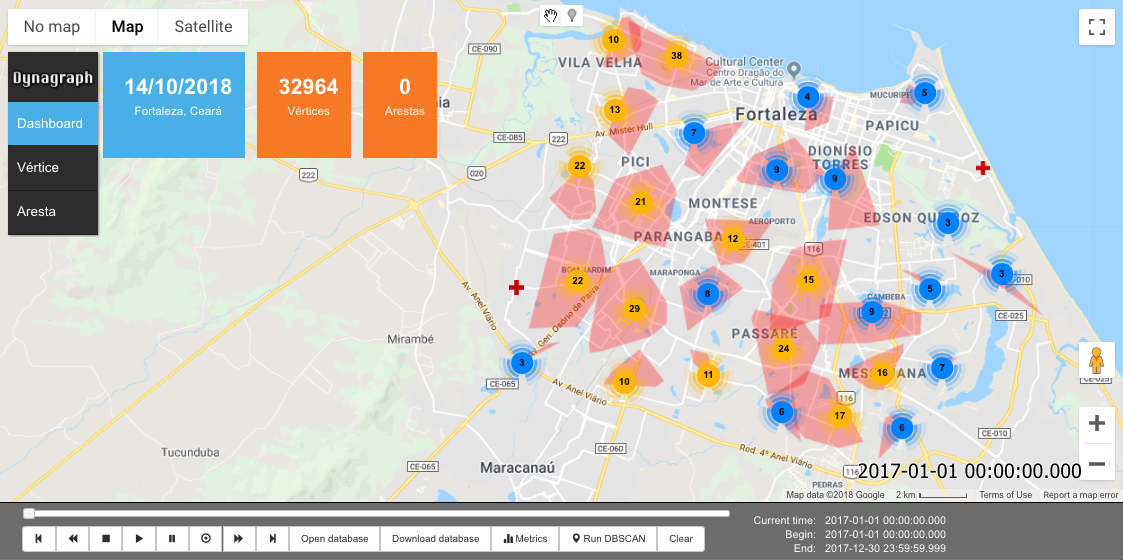
\includegraphics[width=15cm]{figuras/editorCaract/edCaractMenu.png}
	}{
		\Fonte{Elaborado pelo autor}
	}
\end{figure}
\FloatBarrier

Para criar um novo vértice, deve-se selecionar o submenu relacionado a vértices como mostra a figura \ref{fig:edCaCriacao1}.
\begin{figure}[!ht]
	\centering	
	\Caption{\label{fig:edCaCriacao1} Editor de Características: criação de um vértice}	
	\UECEfig{}{
		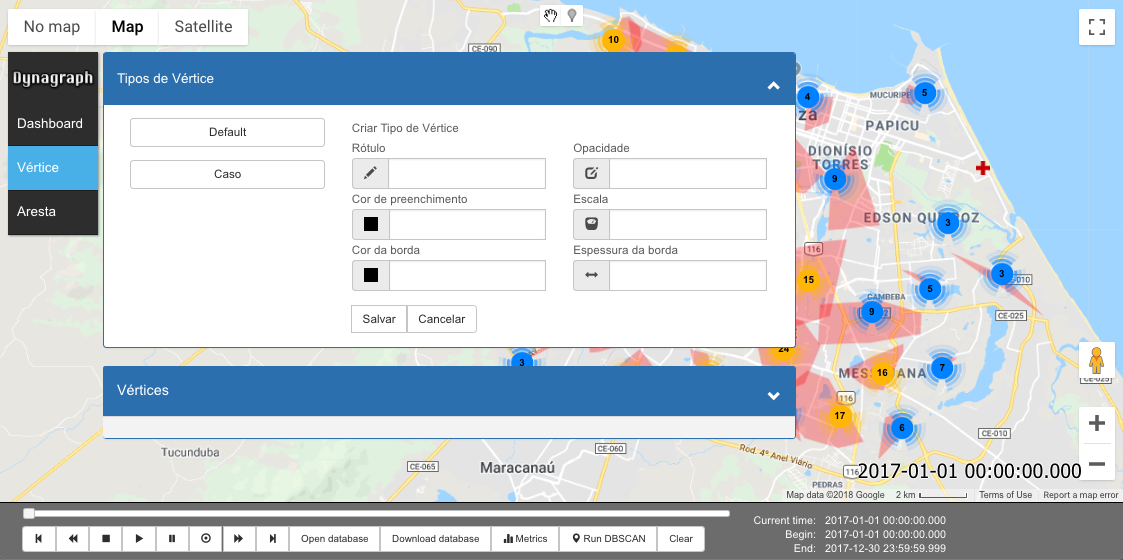
\includegraphics[width=15cm]{figuras/editorCaract/1edCaractCreateVertice.png}
	}{
		\Fonte{Elaborado pelo autor}
	}
\end{figure}
\FloatBarrier

A figura \ref{fig:edCaCriacao2} exibe os tipos de dados permitidos na criação ou edição de um vértice.
\begin{figure}[!ht]
	\centering	
	\Caption{\label{fig:edCaCriacao2} Editor de Características: criação de um vértice - tipos de dados}	
	\UECEfig{}{
		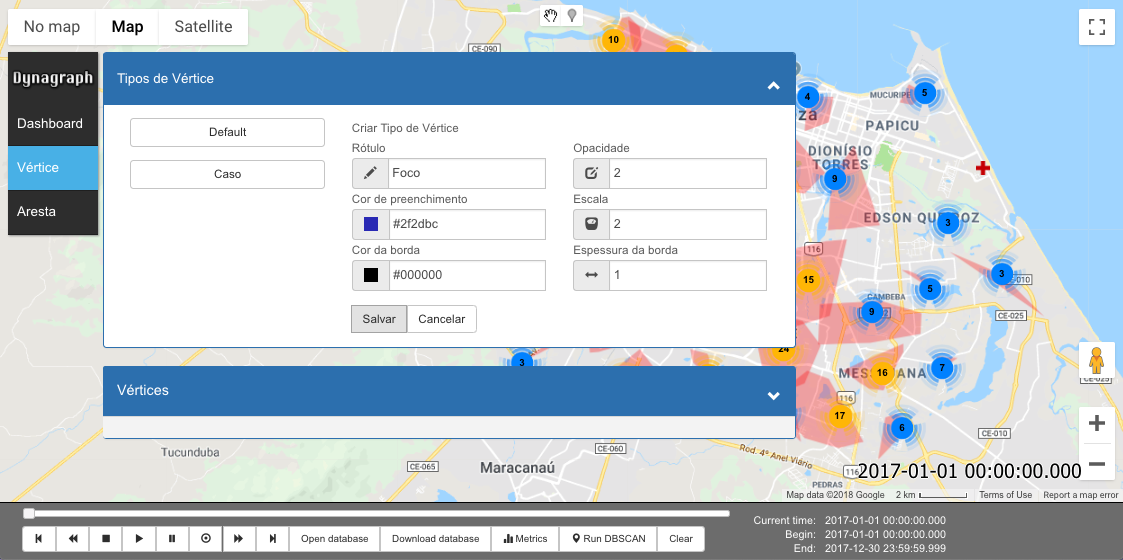
\includegraphics[width=15cm]{figuras/editorCaract/2edCaractCreateVertice.png}
	}{
		\Fonte{Elaborado pelo autor}
	}
\end{figure}
\FloatBarrier

Após criar um novo tipo de vértice é possível usá-lo editando um dado ponto no mapa, como mostram as figuras \ref{fig:edCaChangeV1} e \ref{fig:edCaChangeV2}. A figura \ref{fig:edCaShowV} exibe o resultado esperado.
\begin{figure}[!ht]
	\centering	
	\Caption{\label{fig:edCaChangeV1} Editor de Características: edição de um vértice - parte 1}	
	\UECEfig{}{
		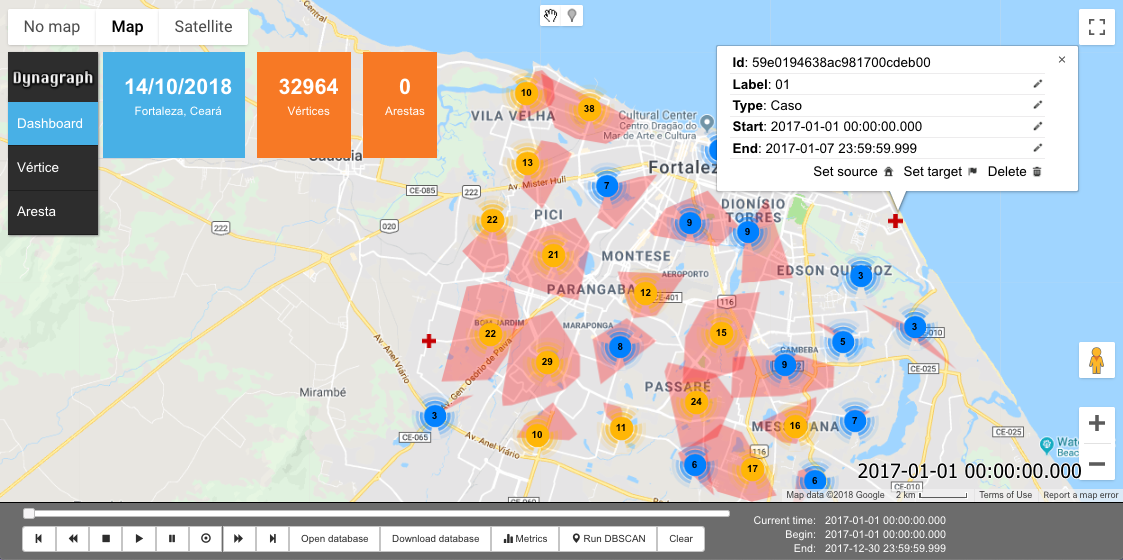
\includegraphics[width=15cm]{figuras/editorCaract/3edCaractChangeVertice.png}
	}{
		\Fonte{Elaborado pelo autor}
	}
\end{figure}
\FloatBarrier

\begin{figure}[!ht]
	\centering	
	\Caption{\label{fig:edCaChangeV2} Editor de Características: edição de um vértice - parte 2}	
	\UECEfig{}{
		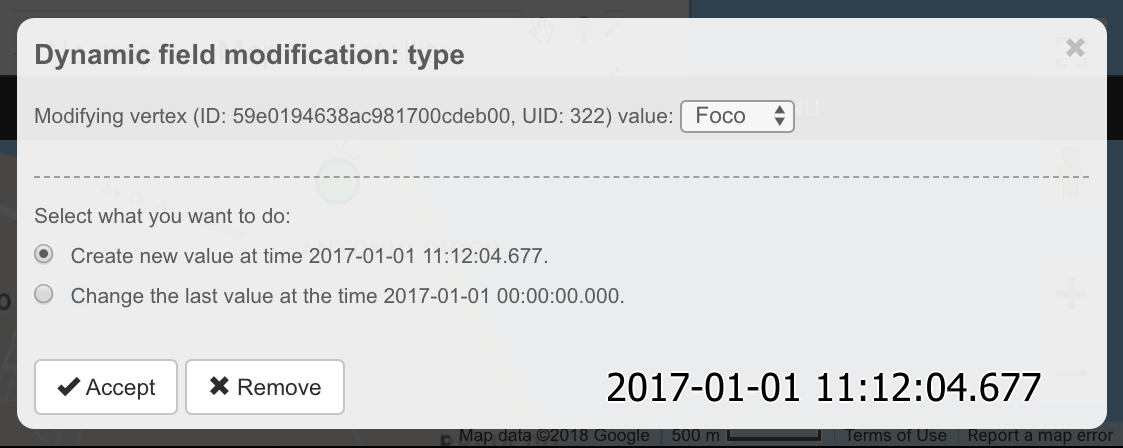
\includegraphics[width=15cm]{figuras/editorCaract/4edCaractChangeVertice.png}
	}{
		\Fonte{Elaborado pelo autor}
	}
\end{figure}
\FloatBarrier

\begin{figure}[!ht]
	\centering	
	\Caption{\label{fig:edCaShowV} Editor de Características: edição de um vértice - parte 3}	
	\UECEfig{}{
		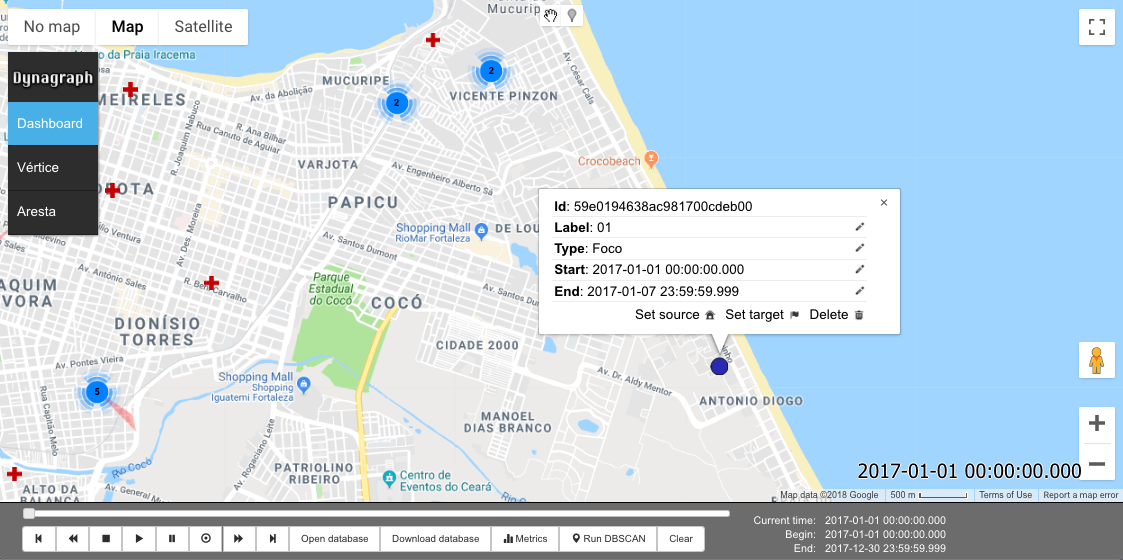
\includegraphics[width=15cm]{figuras/editorCaract/5edCaractShowVertice.png}
	}{
		\Fonte{Elaborado pelo autor}
	}
\end{figure}
\FloatBarrier

Para editar um tipo de vértice basta selecioná-lo a partir da lista de tipos de vértices e então aplicar as mudanças, como mostra a figura \ref{fig:edCaEditV1} e o resultado na figura \ref{fig:edCaEditV2}.
\begin{figure}[!ht]
	\centering	
	\Caption{\label{fig:edCaEditV1} Editor de Características: edição de um tipo de vértice - parte 1}	
	\UECEfig{}{
		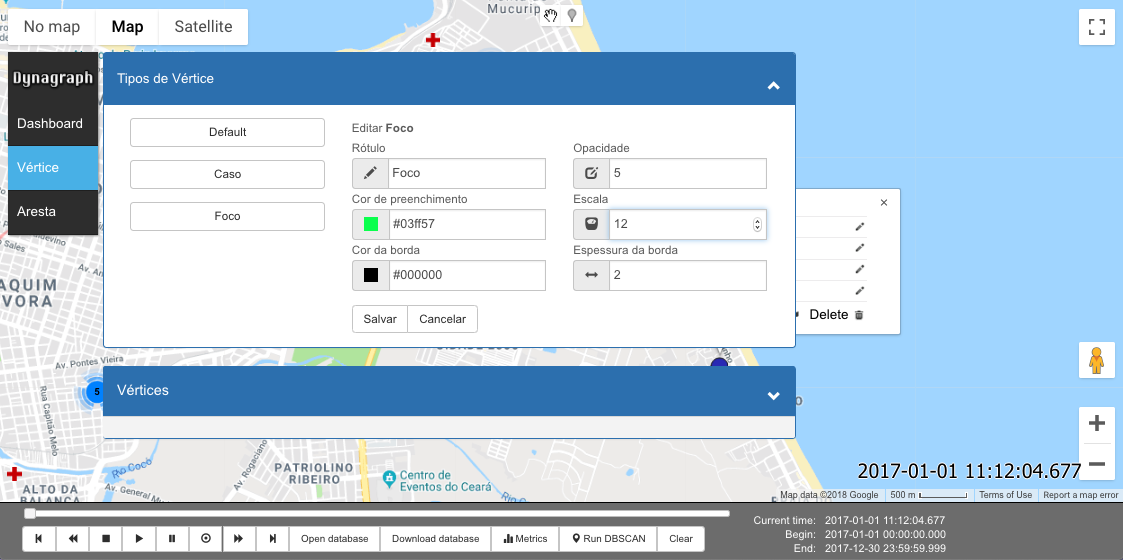
\includegraphics[width=15cm]{figuras/editorCaract/6edCaractEditVertice.png}
	}{
		\Fonte{Elaborado pelo autor}
	}
\end{figure}
\FloatBarrier
\begin{figure}[!ht]
	\centering	
	\Caption{\label{fig:edCaEditV2} Editor de Características: edição de um tipo de vértice - parte 2}	
	\UECEfig{}{
		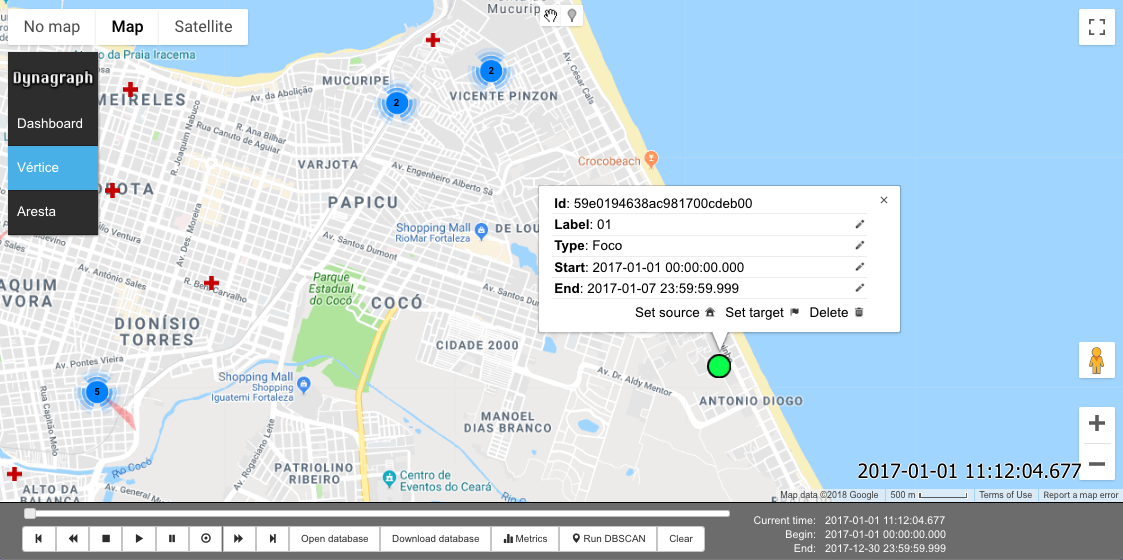
\includegraphics[width=15cm]{figuras/editorCaract/7edCaractEditedVertice.png}
	}{
		\Fonte{Elaborado pelo autor}
	}
\end{figure}
\FloatBarrier

Outra opção de edição de um vértice é dada na figura \ref{fig:edCaractEditVerticeOption2}. Nesta opção pode-se usar uma imagem pronta.
\begin{figure}[!ht]
	\centering	
	\Caption{\label{fig:edCaractEditVerticeOption2} Editor de Características: Tipo de vértice}	
	\UECEfig{}{
		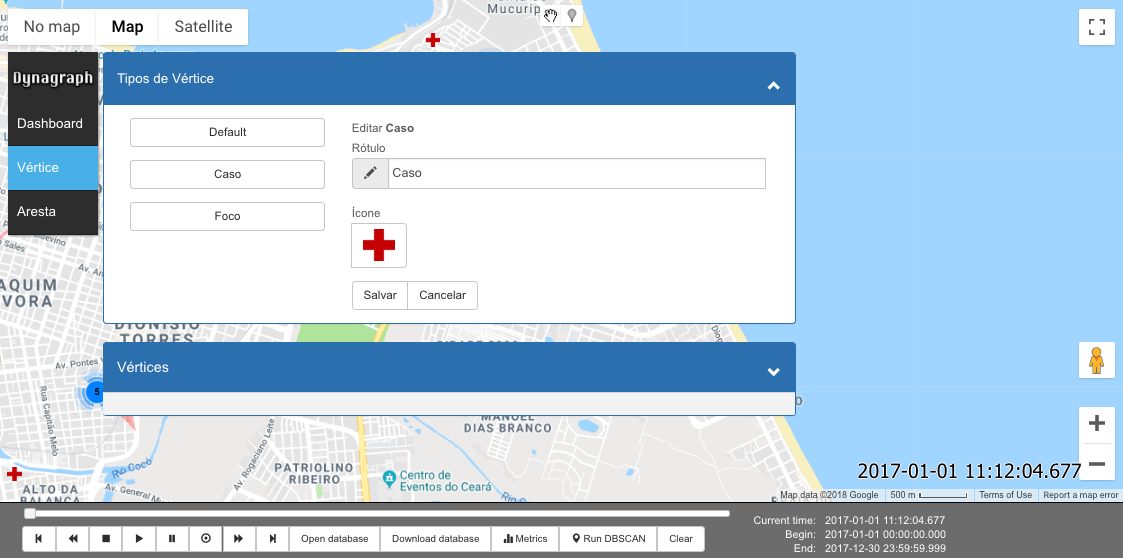
\includegraphics[width=15cm]{figuras/editorCaract/edCaractEditVerticeOption2.png}
	}{
		\Fonte{Elaborado pelo autor}
	}
\end{figure}
\FloatBarrier

O Editor de Características permite também a criação e edição de arestas (figura \ref{fig:edCaractAresta}), mas essa funcionalidade não foi necessária nesta pesquisa.
\begin{figure}[!ht]
	\centering	
	\Caption{\label{fig:edCaractAresta} Editor de Características: Aresta}	
	\UECEfig{}{
		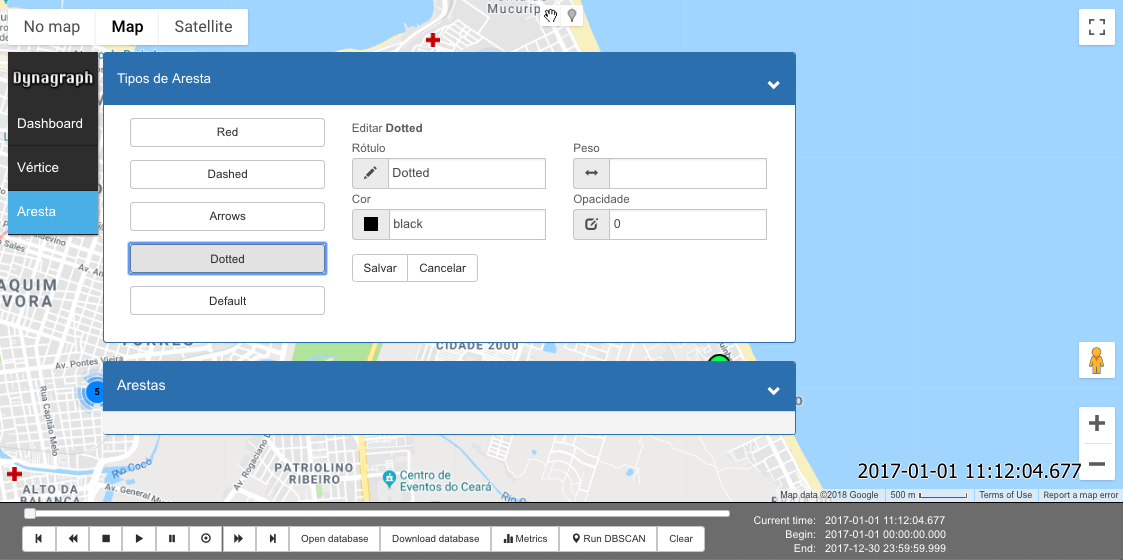
\includegraphics[width=15cm]{figuras/editorCaract/edCaractAresta.png}
	}{
		\Fonte{Elaborado pelo autor}
	}
\end{figure}
\FloatBarrier

\subsubsection{Visualização dos grupos formados}

Foram usados dois algoritmos para permitir a visualização dos grupos formados em um dado tempo. O primeiro é uma biblioteca proveniente das APIs do Google chamada MarkerClusterer \cite{markerCluster}, que cria e gerencia grupos de acordo com o nível de \textit{zoom} para grandes quantidades de pontos. Essa biblioteca é combinada com a API Javascript do Google Maps$^{TM}$ para agrupar os pontos por proximidade e simplificar a exibição dos pontos no mapa.
De acordo com o nível de \textit{zoom} os grupos são formados com cores e tamanhos diferentes, como mostram as figuras \ref{fig:apiGoogleMaps1} e \ref{fig:apiGoogleMaps2}.
\begin{figure}[!ht]
	\centering	
	\Caption{\label{fig:apiGoogleMaps1} Grupos - API Google Maps parte 1}	
	\UECEfig{}{
		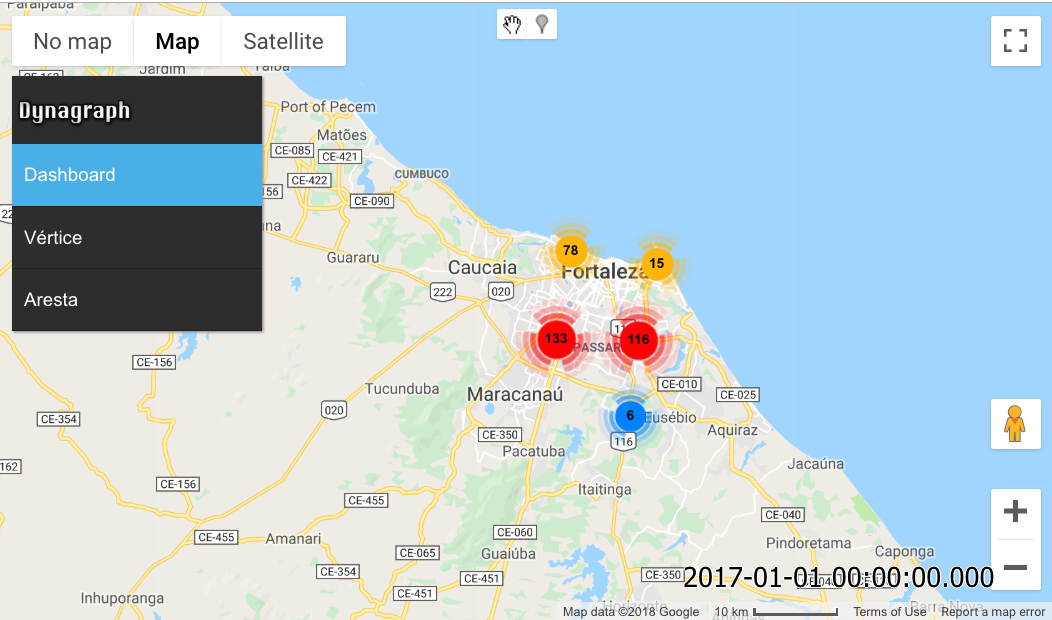
\includegraphics[width=13cm]{figuras/ClusterAPIGoogle1.png}
	}{
		\Fonte{Elaborado pelo autor}
	}
\end{figure}
\FloatBarrier

\begin{figure}[!ht]
	\centering	
	\Caption{\label{fig:apiGoogleMaps2} Grupos - API Google Maps parte 2}	
	\UECEfig{}{
		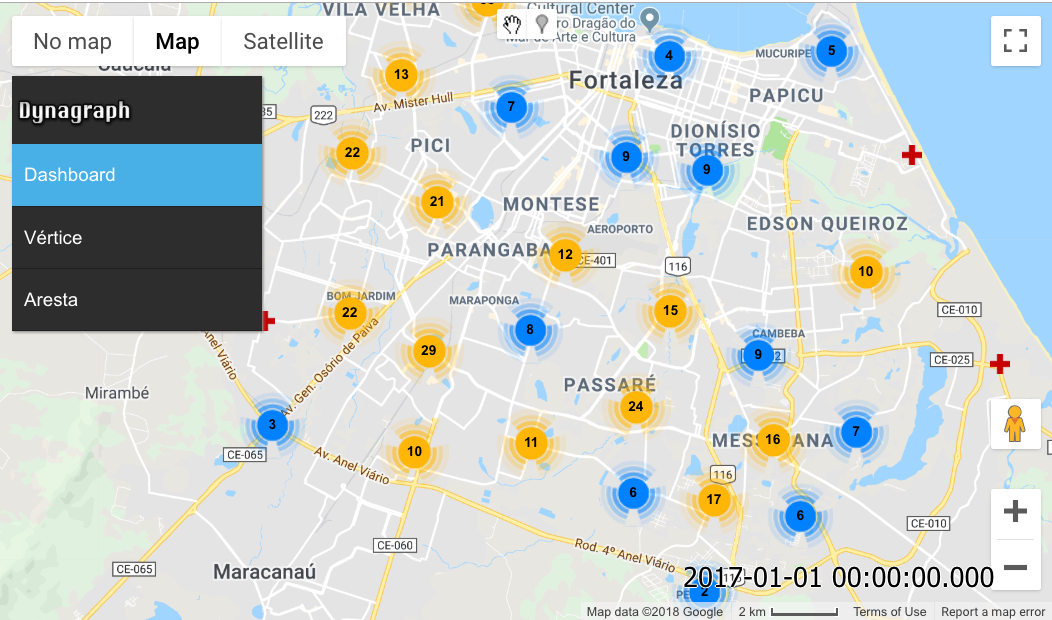
\includegraphics[width=13cm]{figuras/ClusterAPIGoogle2.png}
	}{
		\Fonte{Elaborado pelo autor}
	}
\end{figure}
\FloatBarrier

O segundo algoritmo é conhecido como {\em Convex Hull} \cite{ConvexHull}. Também denominado de fecho convexo. No problema é dado um conjunto de pontos em um espaço e deseja-se encontrar o menor número de pontos que geram um polígono convexo no qual abranja todos os outros pontos.
As figuras \ref{fig:algConvexHull1} e \ref{fig:algConvexHull2} apresentam exemplos do \emph{convex hull}, onde cada polígono representa o grupo de casos de dengue naquela região delimitada. Dos vários pontos, somente os pontos mais externos é que formam o menor polígono que engloba todos os outros pontos.
%
\begin{figure}[!ht]
	\centering	
	\Caption{\label{fig:algConvexHull1} Exemplo 1 de Convex Hull}	
	\UECEfig{}{
		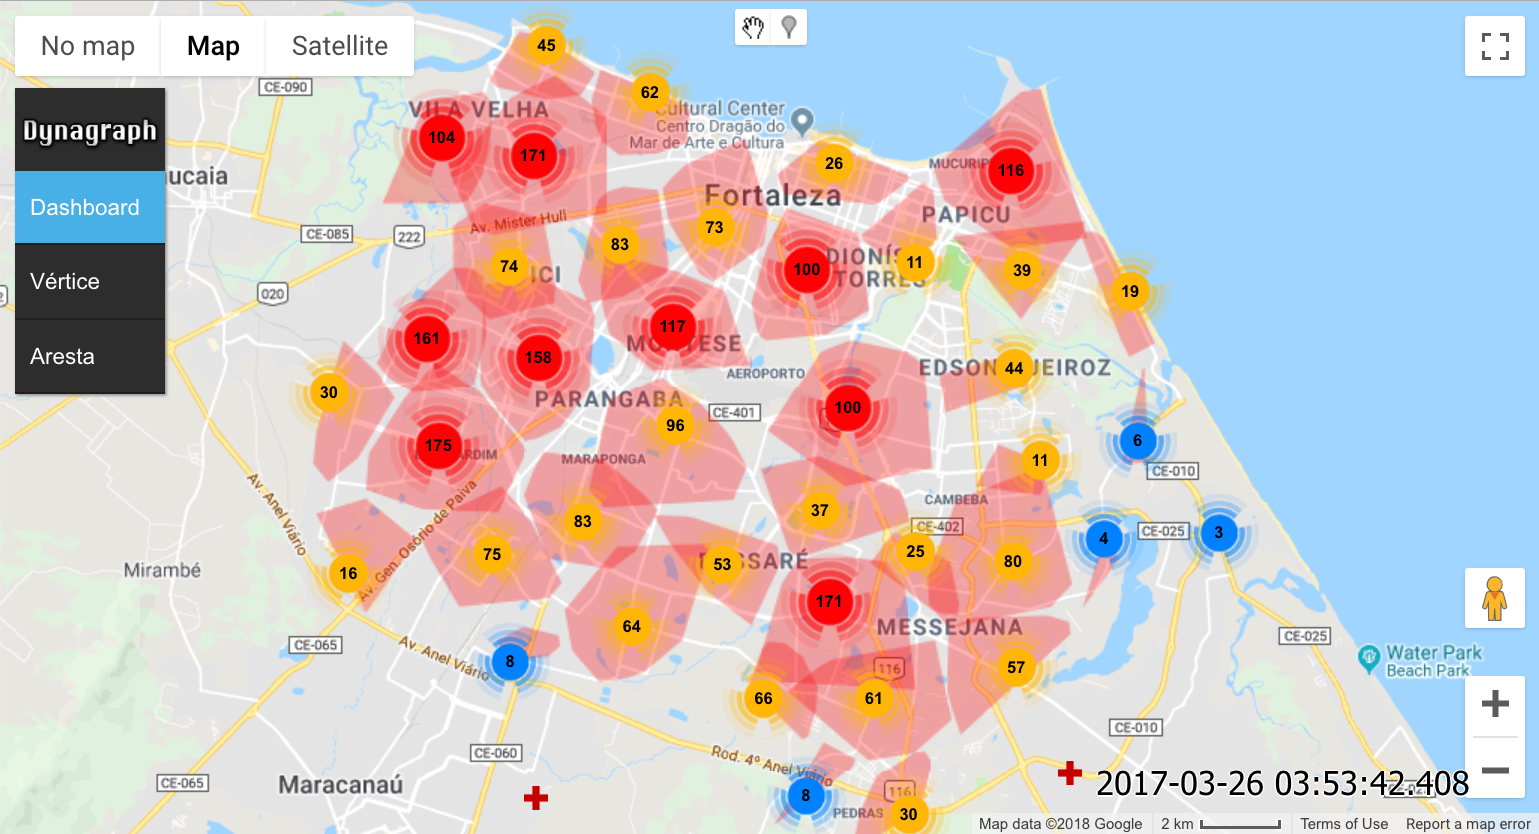
\includegraphics[width=14cm]{figuras/algConvexHull1.png}
	}{
		\Fonte{Elaborado pelo autor}
	}
\end{figure}
\FloatBarrier
\begin{figure}[!ht]
	\centering	
	\Caption{\label{fig:algConvexHull2} Exemplo 2 de Convex Hull}	
	\UECEfig{}{
		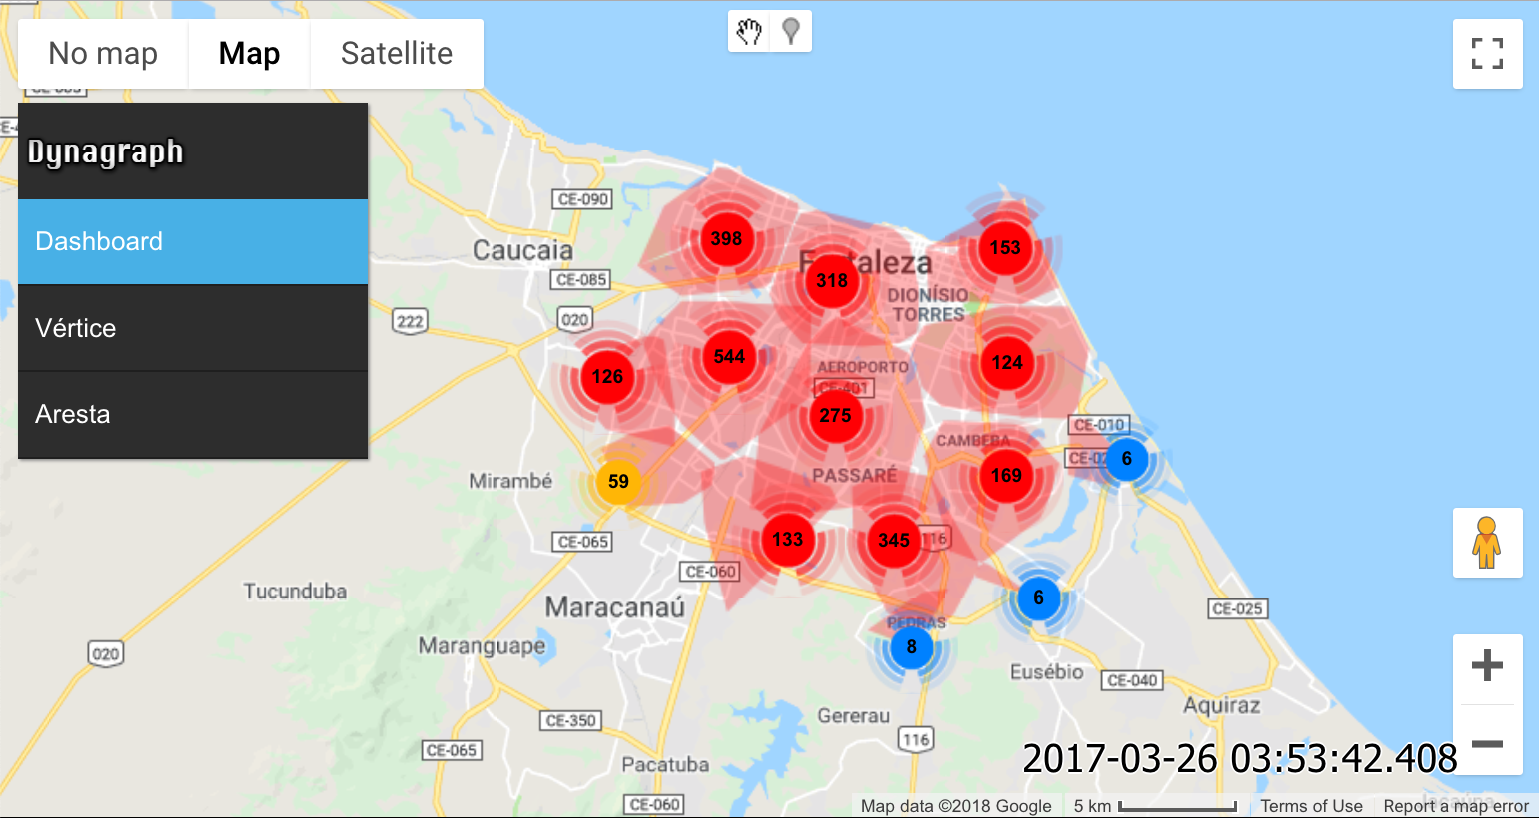
\includegraphics[width=14cm]{figuras/algConvexHull2.png}
	}{
		\Fonte{Elaborado pelo autor}
	}
\end{figure}
\FloatBarrier
    \section{Estudos Relacionados e Escolha de Métodos Dinâmicos}
\label{sec:trabalhos-relacionados}

% TODO: melhorar este capítulo - Pesquisa que não fizemos

\subsection{Estudos Relacionados}
\label{subsec:estudos}

\subsection{Escolha dos Métodos Dinâmicos}
\label{subsec:metodos-escolhidos}

Como vimos na seção anterior há uma carência de estudos relacionando os assuntos abordados: agrupamento, previsão em dados dinâmicos espaço-temporais, grafos dinâmicos e sistemas web de forma integrada. Deste modo foi necessário dividir o problema de agrupamentos e previsões dinâmicos em três etapas:
\begin{itemize}
\item Estrutura de dados em grafos dinâmicos.
\item Modelos de previsão espaço-temporais.
\item Algoritmos de agrupamento dinâmico.
\end{itemize}

Esta pesquisa aborda nas seções anteriores deste capítulo a estrutura de dados em grafos dinâmicos usando passos já descritos na literatura, principalmente o modelo Dynagraph \cite{dynagraph}, que é baseado na primeira proposta em \cite{dynagraph2012}, onde o Dynagraph usa sequências temporais para vértices, arestas, características modificáveis dos vértices e arestas e o relacionamento entre suas características. Ele permite formar um grafo com as informações necessárias para qualquer instante no tempo. 

O algoritmo de agrupamento dinâmico \acrshort{ST-DBSCAN} tem como base o algoritmo \acrshort{DBSCAN}, o qual possui a capacidade de descobrir agrupamentos de acordo com valores não espaciais, espaciais e temporais dos objetos. Com ele é possível descobrir grupos em dados espaciais-temporais baseado na densidade das ocorrência dos objetos. Tais agrupamentos se caracterizam por se distribuem em massas compactas, pois são baseadas em densidade. Logo, este método pode ser usado no contexto da descoberta de grupos para o conjunto de dados espaço-temporais de casos humanos de arboviroses, dada a forma como elas se expandem. 

O método \acrshort{ST-IGN} consiste da aplicação do método \acrshort{IGN} estático \cite{simposioNeg2003} sobre cada uma das $n$ instâncias (estados) geradas a partir de um período (intervalo fixo de estados) definido pelo processo de identificação da dinâmica do comportamento dos objetos. O método rotula os grupos naturais encontrados na unidade de tempo $i$ com base na máxima densidade de objetos que se mantém no mesmo grupo após uma divisão e/ou aglomeração.

Os dois algoritmos apresentados são utilizados como base para os modelos de previsão espaço-temporais. Um modelo simples de previsão é implementado, o qual se basea no histórico dos grupos, a partir do centro e do raio dos grupos em análise, onde o centro e o raio são definidos de acordo com a média da posição dos objetos de cada grupo identificado no tempo. Dos grupos identificados como sendo de mesma origem no tempo são então tomados seus valores médios de seus centros e raios, gerando finalmente o grupo de previsão do próximo intervalo. O método \acrshort{ST-IGN} em especial tem a vantagem da separabilidade dos grupos naturais, caso exista de forma bem definida, como foi mostrado no capítulo \ref{chap:estadodaarte}, além disto este método consegue descobrir grupos que se formam em linha e mesmo em massa, apesar da desvantagem de formar grandes grupos quando as distãncias são muito pequenas entre objetos.

Uma vez que é bastante assertivo nos grupos que forma, não importando a quantidade de dados, trata-se de um método que pode ser considerado para avaliação, haja vista sua liberdade em encontrar grupos de várias formas permitindo-nos abrir a caracterização de padrões de comportamento das arboviroses, além das hoje consideradas pela literatura.
	\chapter{Modelos de agrupamento e previsão em redes dinâmicas}
\label{chap:modelo-agrupamento}

\section{Modelo de previsão baseado nos clusters anteriores (centro e raio)}

Este modelo gera grupos de previsão baseados no histórico dos grupos, nos centros geométricos dos grupos em análise e no raio de acordo com a média do número de casos de dengue de cada grupo.

As figuras \ref{fig:stdbscan1}, \ref{fig:stdbscan2} e \ref{fig:stdbscan3} exibem os grupos formados pelo ST-DBSCAN, onde os dados tomados de exemplo são casos de dengue de janeiro de 2017.
A figura \ref{fig:stdbscan3} exibe também os grupos de predição formados pelo grupo 55 e 57.

\begin{figure}[!ht]
	\centering	
	\Caption{\label{fig:stdbscan1} ST-DBSCAN: Semana 1}
	\UECEfig{}{
		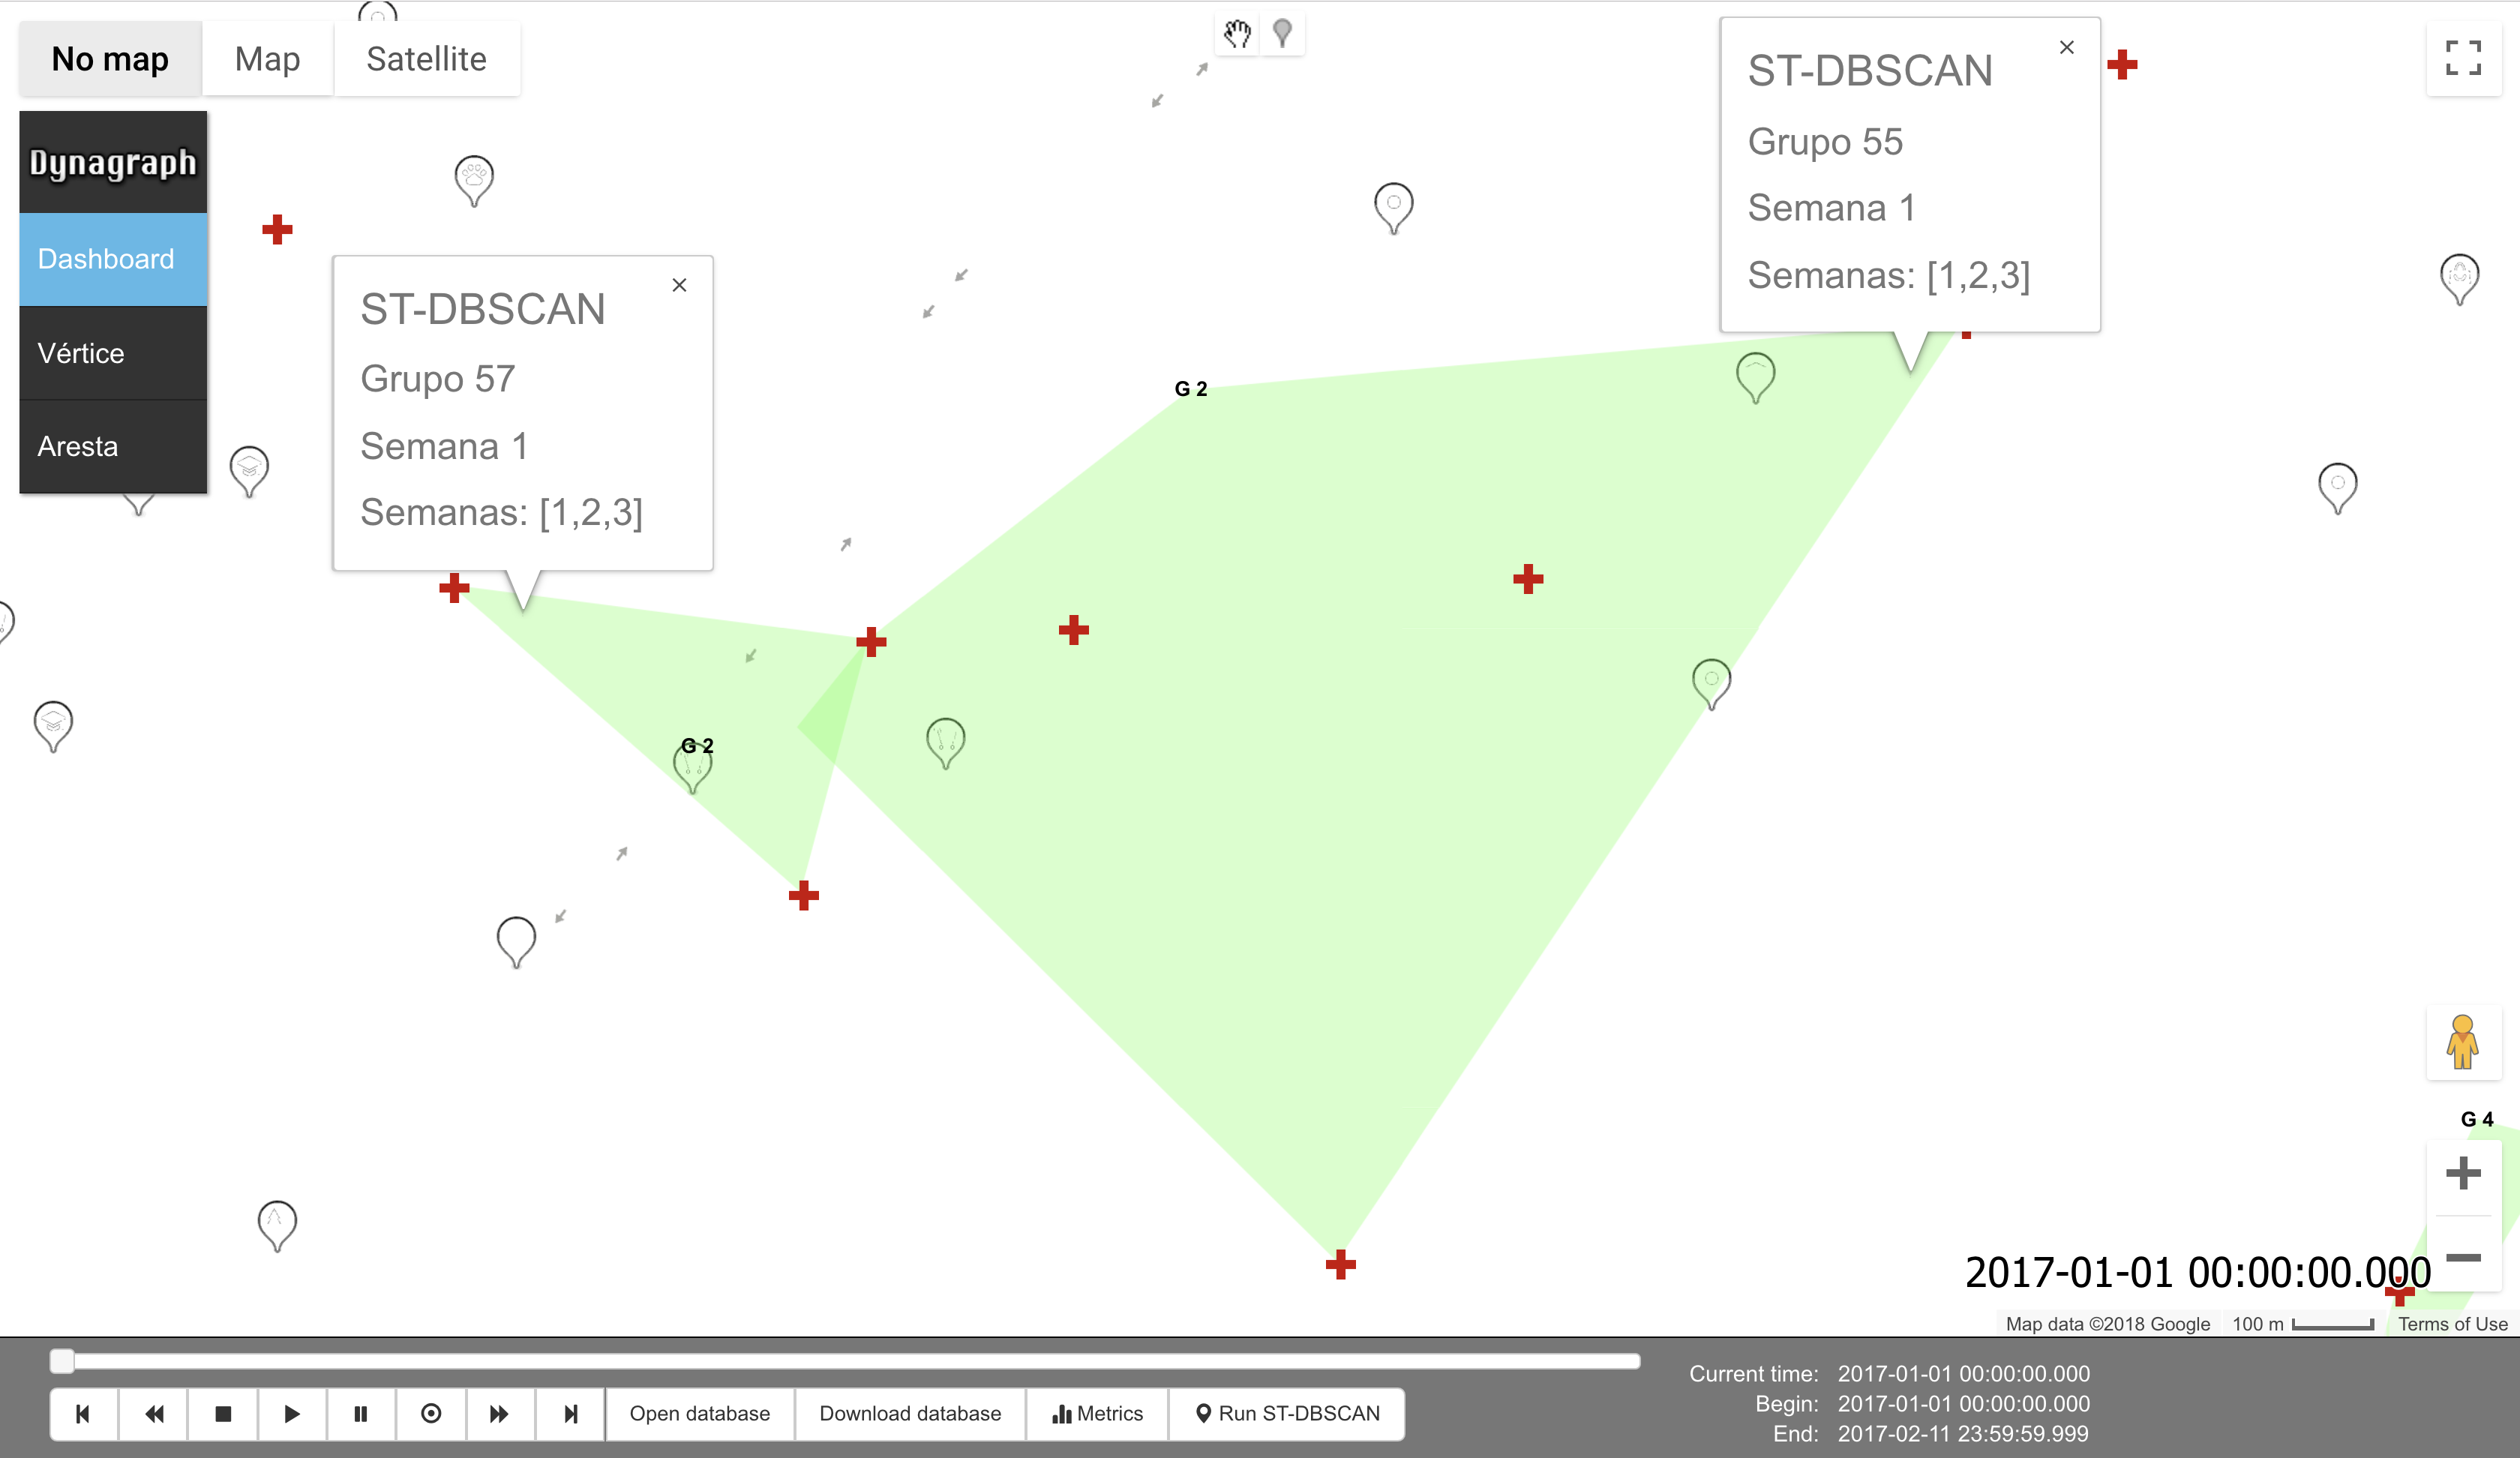
\includegraphics[width=15cm]{figuras/stdbscan/stdbscan1.png}
	}{
		\Fonte{Elaborado pelo autor}
	}
\end{figure}
\FloatBarrier

\begin{figure}[!ht]
	\centering	
	\Caption{\label{fig:stdbscan2} ST-DBSCAN: Semana 2}
	\UECEfig{}{
		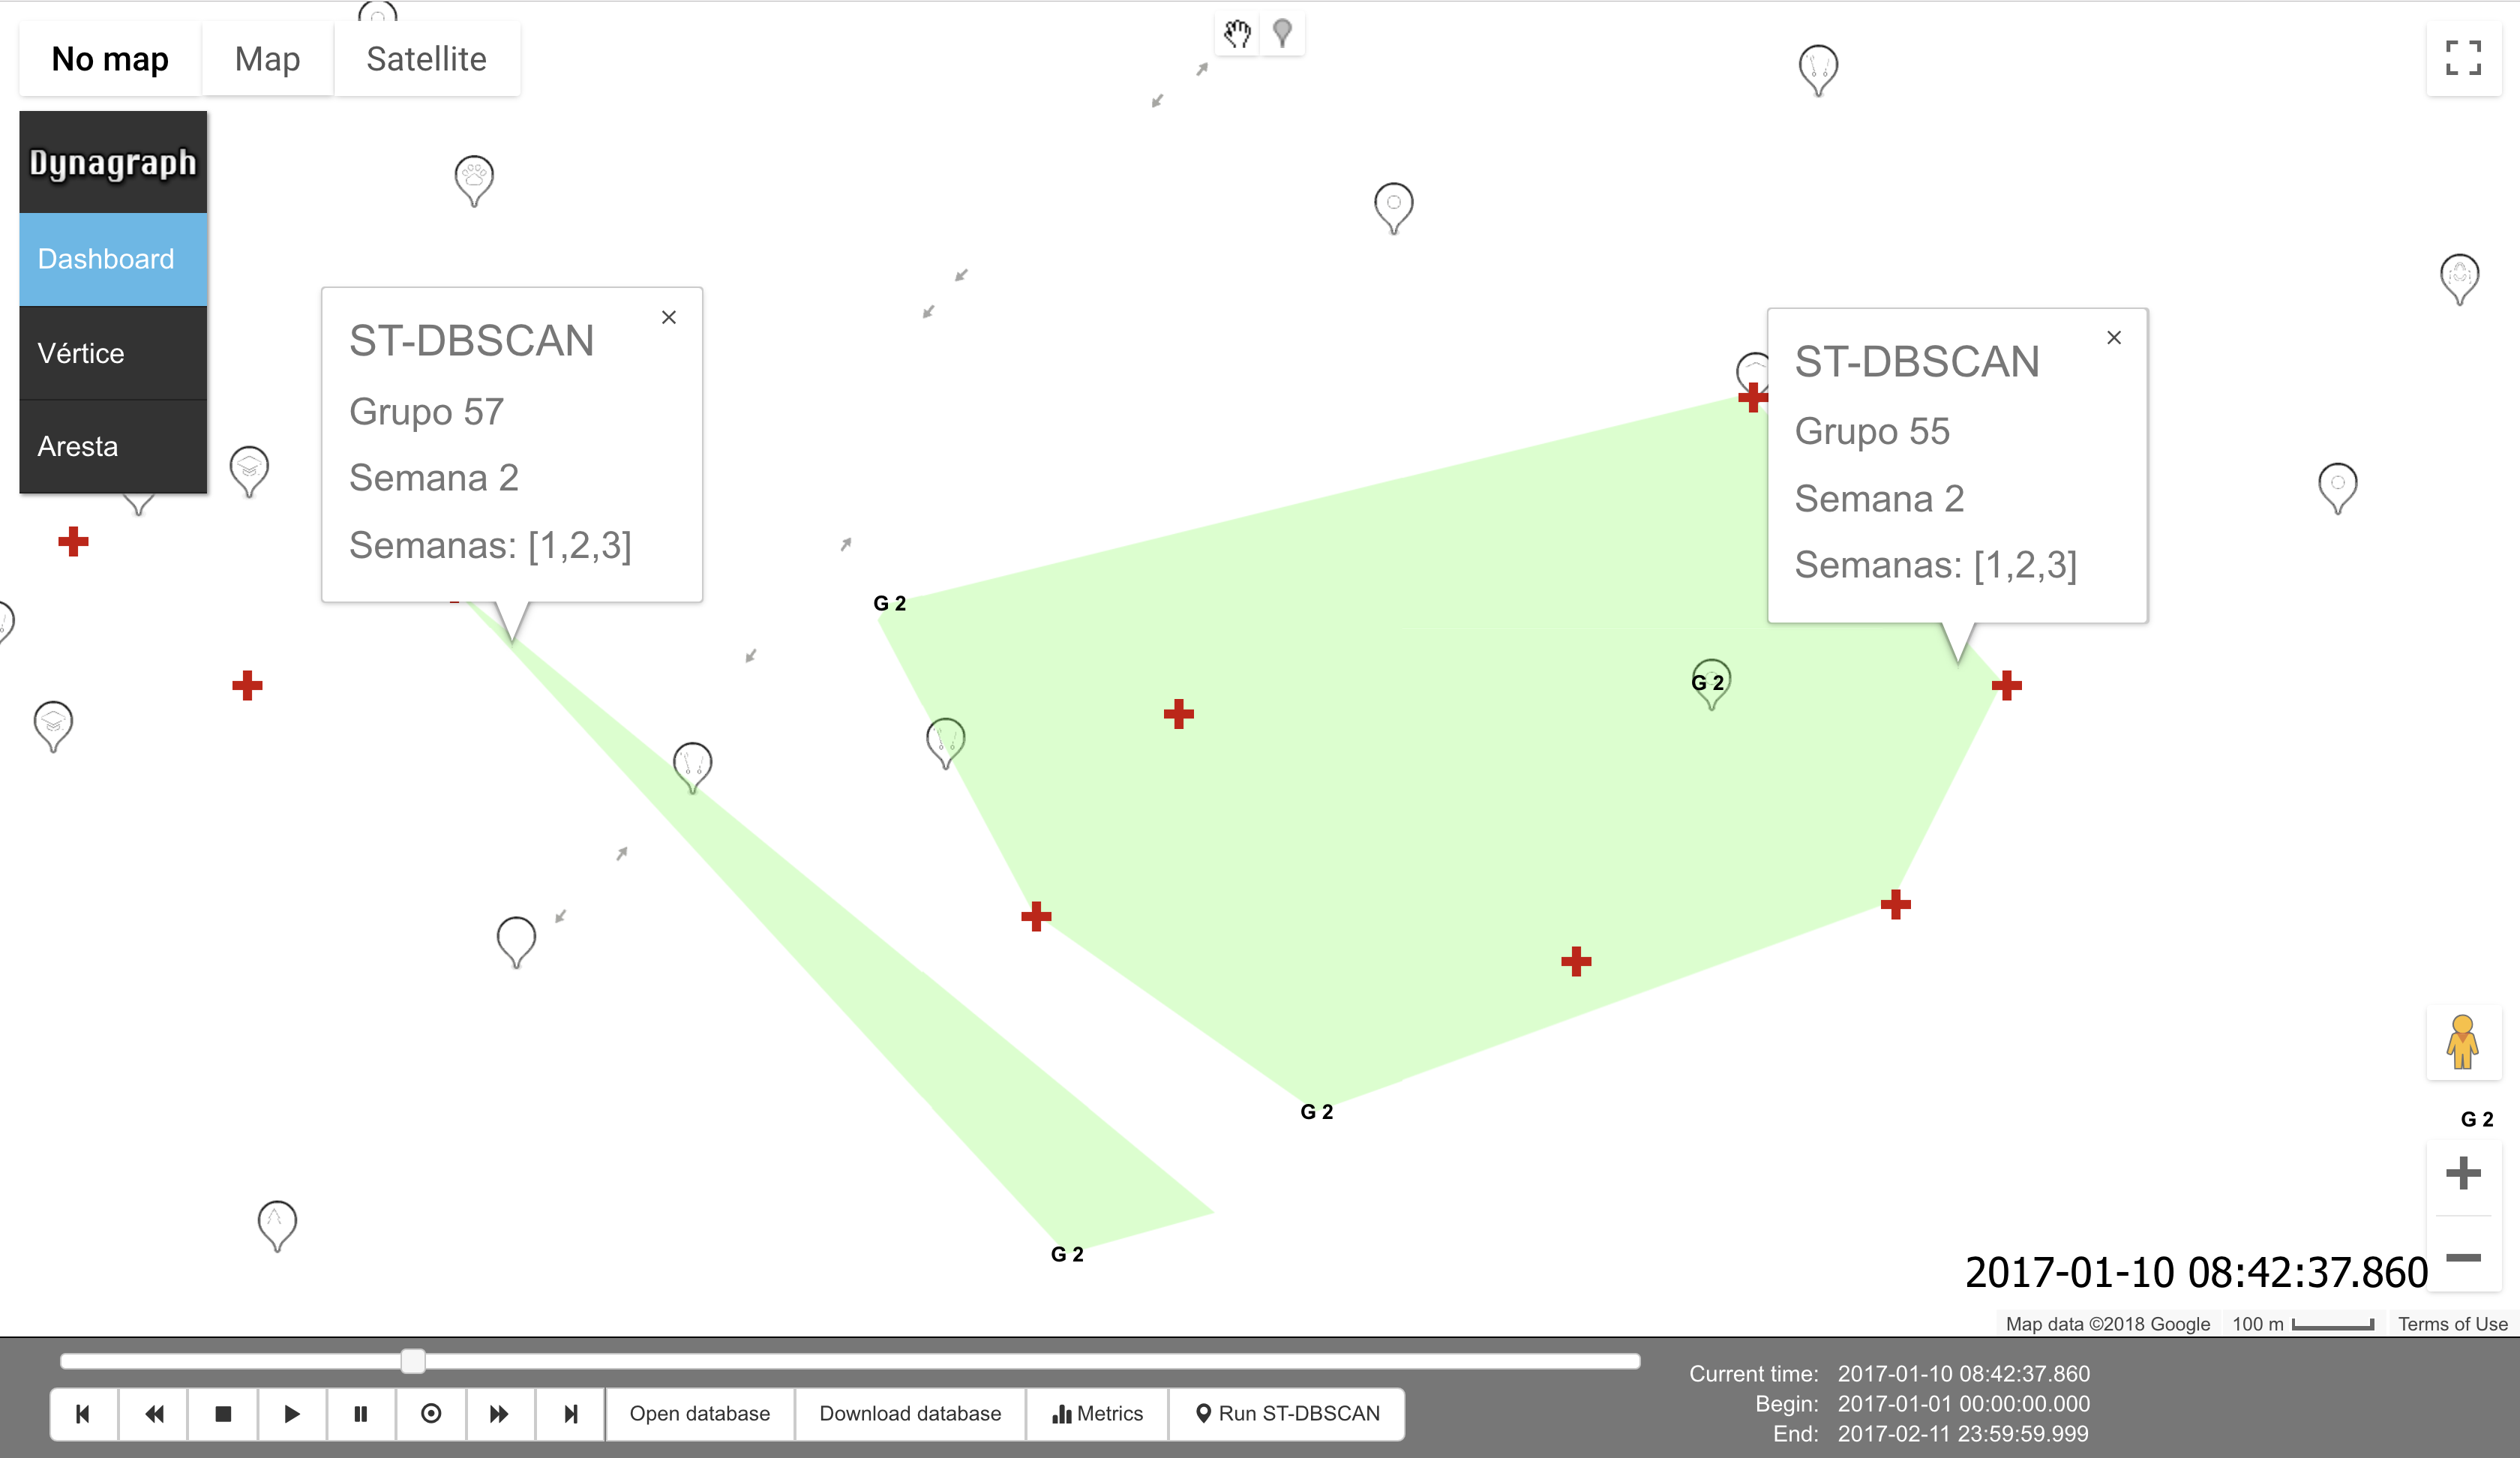
\includegraphics[width=15cm]{figuras/stdbscan/stdbscan2.png}
	}{
		\Fonte{Elaborado pelo autor}
	}
\end{figure}
\FloatBarrier

\begin{figure}[!ht]
	\centering	
	\Caption{\label{fig:stdbscan3} ST-DBSCAN: Semana 3}
	\UECEfig{}{
		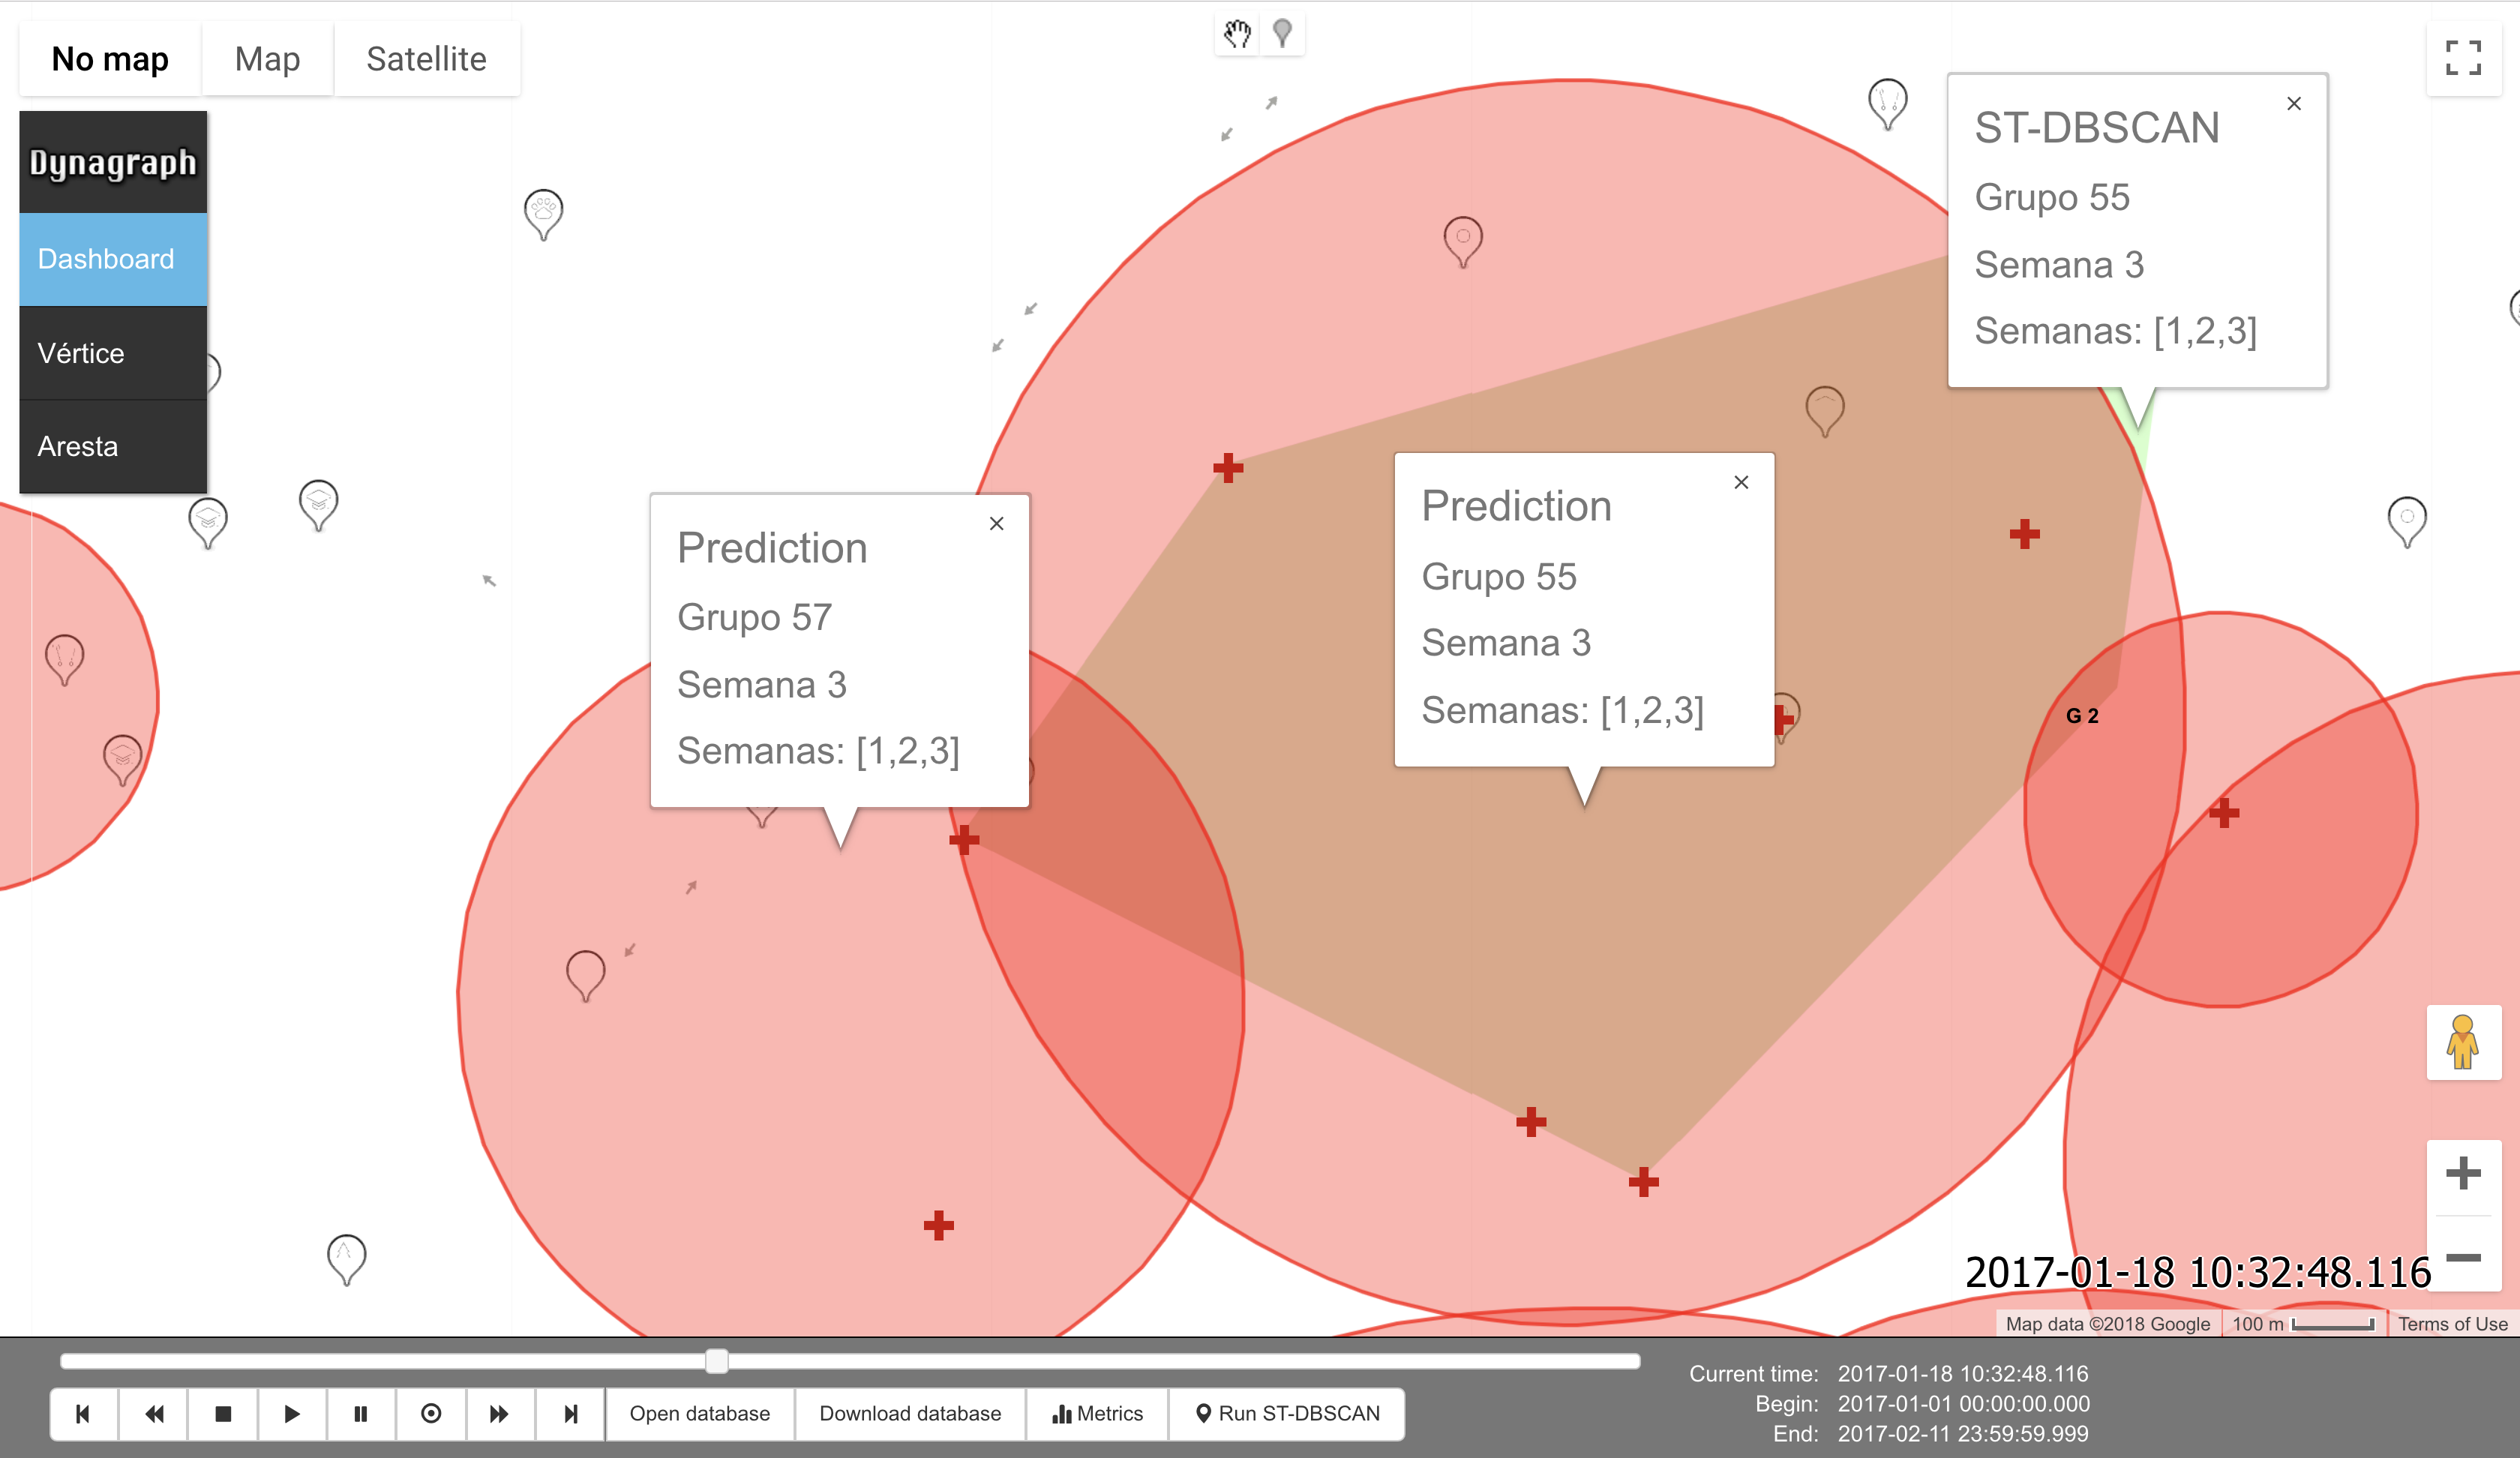
\includegraphics[width=15cm]{figuras/stdbscan/stdbscan3.png}
	}{
		\Fonte{Elaborado pelo autor}
	}
\end{figure}
\FloatBarrier
	\chapter{Uma Solução e sua Aplicação na Previsão de Dengue e Chikungunya em Fortaleza/CE}
\label{chap:avaliacao}
% http://www.ppgia.pucpr.br/~fabricio/ftp/Aulas/Mestrado/IA/Nievola/MD/MD-06-Agrupamento.pdf

Este capítulo apresenta a metodologia computacional empregada nesta pesquisa, que permite orquestrar os dados espaço-temporais provenientes de bases de dados (\acrshort{SIMDA} - \cite{simda} e WebDengue - \cite{webdengue2011}) para o Armazém de Dados (\acrshort{DW} - \textit{\acrlong{DW}}) e tratá-los de modo a se tornarem informação e recursos de tomada de decisão com os modelos de agrupamento dinâmico através do Dynagraph. Em seguida, trata-se dos resultados obtidos com os modelos de previsão estudados usando os algoritmos \acrshort{ST-DBSCAN} e \acrshort{ST-IGN}.

\section{Metodologia Computacional para Previsão de Grupos}

A figura \ref{fig:sad} apresenta a representação do modelo metodológico (metodologia) empregada para tornar factível a leitura, armazenamento, visualização e análise de dados espaço-temporais. A figura \ref{fig:metodologia} representa o \acrshort{SAD} dessa metodologia nos casos de dengue e chikungunya, utilizando o Dynagraph para análise dos dados e a base de dados do \citeonline{simda}.

\begin{figure}[!ht]
	\centering	
	\Caption{\label{fig:sad} Metodologia Computacional}
	\UECEfig{}{
		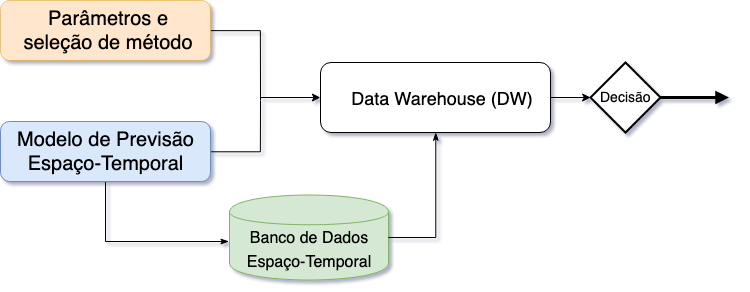
\includegraphics[width=14cm]{figuras/sad.png}
	}{
		\Fonte{Elaborado pelo autor}
	}
\end{figure}
\FloatBarrier

O SAD apresentado na figura \ref{fig:metodologia} mostra um Armazém de Dados composto de um \acrfull{BD-SQL} (\acrfull{SQL}) onde são colocadas as informações dos casos, conforme figura \ref{fig:jsondynagraphVertex}, e o visualizador e editor Dynagraph que permite transformar tais dados em informações úteis no espaço-tempo, como é mostrado nas figuras \ref{fig:jsondynagraphVertex}, \ref{fig:jsondynagraphAresta} e \ref{fig:edCaMenu}.

O banco de dados é alimentado através de um sistema, por exemplo SIMDA e WebDengue, e determinado por um especialista. Para compor uma solução adequada, outro especialista decide o modelo de previsão espaço-temporal baseado no banco de dados e os parâmetros de entrada do modelo. Com isso, uma solução é fornecida ao Dynagraph, que visualiza no espaço-tempo os grupos de previsão. E finalmente, com as informações geradas pelo Armazém de Dados, outro especialista em tomada de decisão determina onde os agentes de saúde devem atuar para um combate mais efetivo às endemias.

\begin{figure}[!ht]
	\centering	
	\Caption{\label{fig:metodologia} Sistema de Apoio a Decisão Espaço-Temporal}
	\UECEfig{}{
		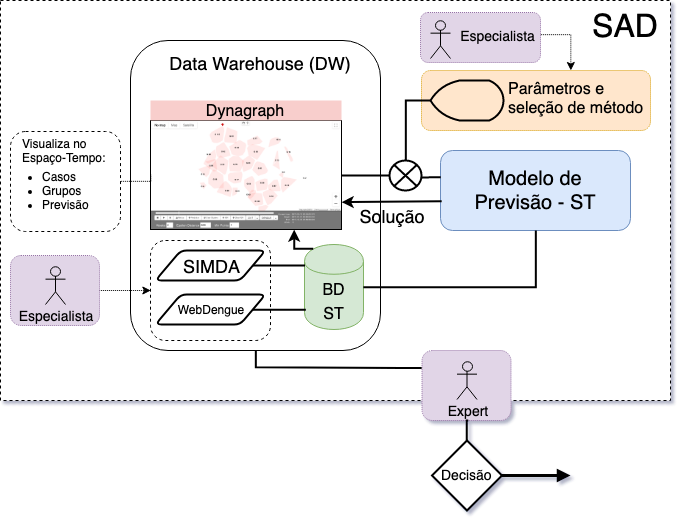
\includegraphics[width=15cm]{figuras/MetodologiaDissertacao.png}
	}{
		\Fonte{Elaborado pelo autor}
	}
\end{figure}
\FloatBarrier

\section{Avaliação da Metodologia}

Para a avaliação da metodologia proposta, diferentes aspectos de validação de grupos são analisados, tais como:
\begin{itemize}
    \item Comparar os resultados de uma análise de grupos com resultados conhecidos;
    \item Indicar se uma estrutura não aleatória realmente existe num conjunto de dados;
    \item Comparar os resultados de dois diferentes métodos de análise de agrupamento espaço-temporal para determinar qual delas é melhor;
    \item Determinar o número de grupos.
\end{itemize}

Para validar a saída gerada pelo processo de agrupamento, recorre-se a critérios de otimalidade pré-estabelecidos que são os seguintes:
\begin{itemize}
    \item o problema possui um conjunto de variáveis manipuláveis no procedimento de busca pelo ótimo, que são as variáveis de decisão do problema;
    \item os valores assumidos pelas variáveis de decisão devem satisfazer um conjunto de restrições, que compõe a região de soluções viáveis do problema;
    \item as variáveis de decisão do problema podem assumir valores pré-estabelecidos.
\end{itemize}

Os critérios de otimalidade são empíricos no que concerne ao processo de agrupamento. Dependem pois do especialista a indicação analítica do que seria o ótimo. Quando se trata de grupos naturais, um maior número de grupos pode significar uma melhor descrição do contexto, assim como um menor número pode também ter o mesmo significado, dependendo da posição (espaço-tempo) em que o observador estiver em relação ao conjunto de dados de análise.

\section{Testes de Predição e análise}

Foram implementados gráficos de séries temporais que são usados para examinar as variações semanais de uma mudança de situação epidemiológica. Com essas métricas, pode-se comparar padrões de dados, como o número total de casos de dengue de uma determinada semana com o número de casos dentro de algum grupo de previsão, definido pelo método proposto com base nas semanas anteriores à semana em análise.

\section{Comparação de predições baseadas em grupos previamente formados}

As figuras \ref{fig:metricasDengue201745001}, \ref{fig:metricasDengue201845001}, \ref{fig:metricasChi201745001} e \ref{fig:metricasChi201845001} apresentam gráficos sobre as ocorrências de casos humanos de dengue e chikungunya reportados em \cite{simda} no município de Fortaleza, nos anos de 2017 e 2018, levando em consideração as 4 semanas anteriores à semana do grupo de previsão. A variável Eps de agregação do \acrshort{ST-DBSCAN} é de 500 metros (Eps=500) e para caracterizar um grupo se considera pelo menos 2 casos humanos (MinPts=2).
As legendas indicam três tipos:
\begin{itemize}
    \item número de casos dentro de algum grupo de previsão, representado pela cor verde;
    \item número de casos fora de algum grupo de previsão, representado pela cor azul;
    \item número total de casos, representado pela cor laranja.
\end{itemize}

A figura \ref{fig:metricasDengue201745001} apresenta uma grande quantidade de casos humanos de dengue dentro de algum grupo de previsão ao longo do ano de 2017.
\begin{figure}[!ht]
	\centering	
	\Caption{\label{fig:metricasDengue201745001} Métricas \acrshort{ST-DBSCAN}: Dengue/2017, 4 semanas, Eps = 500m, MinPts = 2}
	\UECEfig{}{
		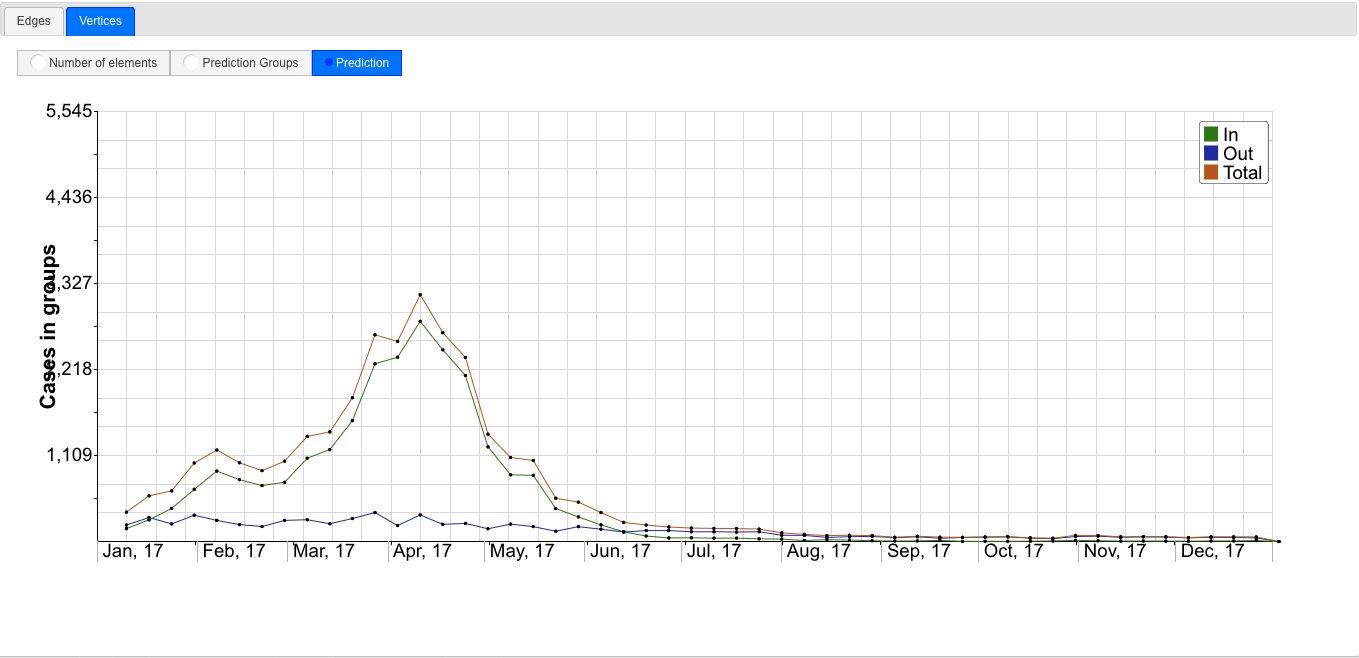
\includegraphics[width=15cm]{figuras/metricas/DENGUE_2017_4_500_1.png}
	}{
		\Fonte{Elaborado pelo autor}
	}
\end{figure}
\FloatBarrier

A figura \ref{fig:agrupamentosDengue2017} representa a seguinte análise:
\begin{itemize}
    \item Casos de dengue em 2017;
    \item Semana 18 do ano;
    \item 1384 casos de dengue na semana de observação;
    \item Semanas  14, 15, 16 e 17 analisadas para gerar os grupos de previsão da semana 18;
    \item 252 grupos de predição gerados;
    \item 208 grupos com pelo menos um caso dentro;
    \item 1220 casos dentro de algum grupo de previsão;
    \item 164 casos fora dos grupos de previsão.
\end{itemize}

Podemos observar que o número de casos dentro de algum grupo de previsão é elevado devido à proximidade entre os grupos, sendo assim, abrangendo grandes áreas com possíveis casos humanos.

\begin{figure}[!ht]
	\centering
	\Caption{\label{fig:agrupamentosDengue2017} Agrupamentos \acrshort{ST-DBSCAN}: Dengue/2017}
	\UECEfig{}{
		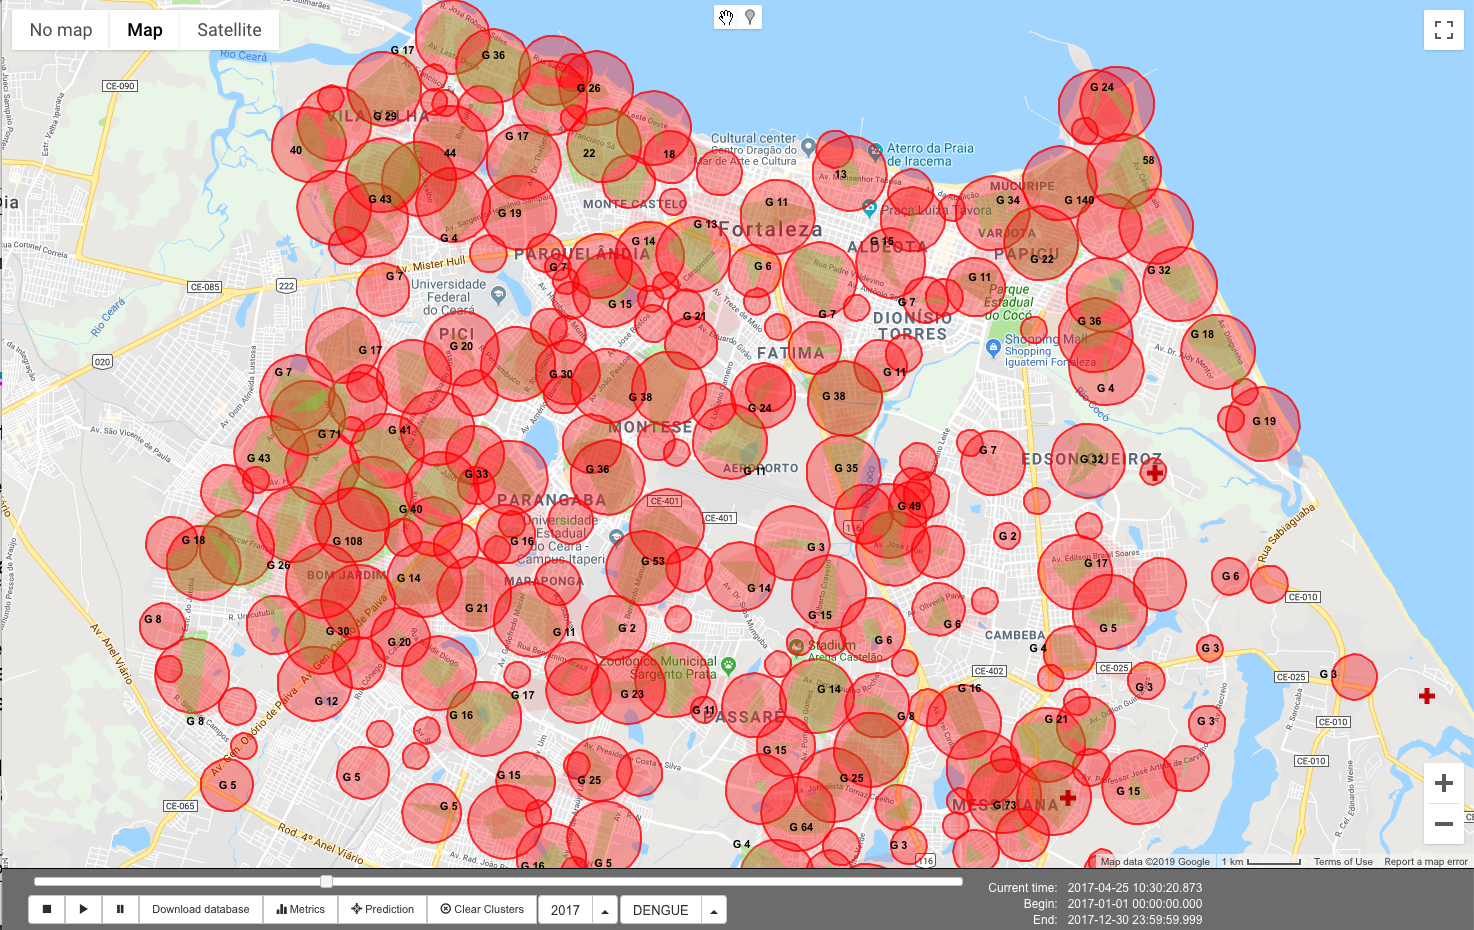
\includegraphics[width=15cm]{figuras/predicao/dbs_dengue2017Week17.png}
	}{
		\Fonte{Elaborado pelo autor}
	}
\end{figure}
\FloatBarrier

O cálculo do raio dos grupos de previsão apresentados é dado por:
${\sqrt[]{p} * 250, p \leqslant 8}$, onde ${p}$ é o número de casos previstos por grupo de previsão gerado pelo \acrshort{ST-DBSCAN}. Logo, o raio máximo dos grupos de previsão da figura \ref{fig:agrupamentosDengue2017} é de aproximadamente 700m.

A figura \ref{fig:metricasDengue201845001} apresenta que o número de casos humanos fora de algum grupo de previsão é maior do que aqueles que estão dentro de algum grupo de previsão, praticamente em todas as semanas analisadas.
\begin{figure}[!ht]
	\centering	
	\Caption{\label{fig:metricasDengue201845001} Métricas \acrshort{ST-DBSCAN}: Dengue/2018, 4 semanas, Eps = 500m, MinPts = 2}
	\UECEfig{}{
		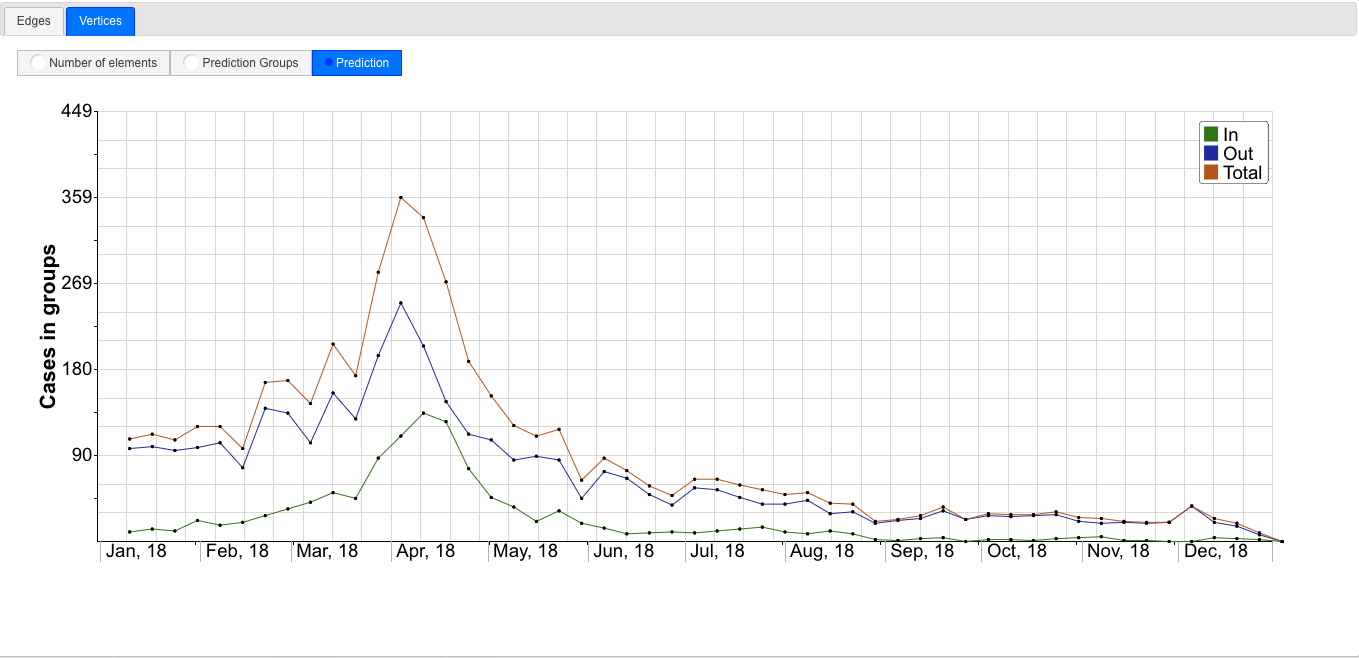
\includegraphics[width=15cm]{figuras/metricas/DENGUE_2018_4_500_1.png}
	}{
		\Fonte{Elaborado pelo autor}
	}
\end{figure}
\FloatBarrier

Observa-se na figura \ref{fig:metricasChi201745001} a semelhança com o gráfico da figura \ref{fig:metricasDengue201745001}, onde é apresentada uma grande quantidade de casos de endemia dentro de uma pequena região. Os grupos de previsão conseguem abranger uma grande área com possíveis casos.
\begin{figure}[!ht]
	\centering	
	\Caption{\label{fig:metricasChi201745001} Métricas \acrshort{ST-DBSCAN}: Chikungunya/2017, 4 semanas, Eps = 500m, MinPts = 2}
	\UECEfig{}{
		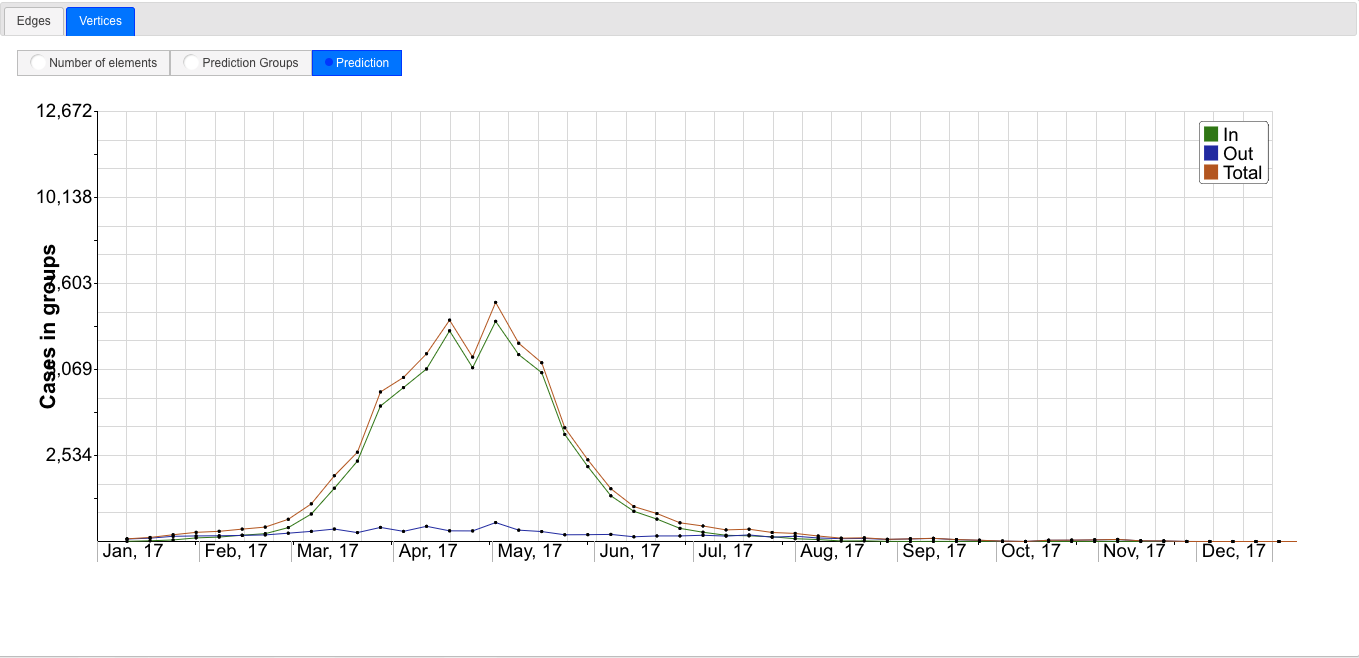
\includegraphics[width=15cm]{figuras/metricas/CHI_2017_4_500_1.png}
	}{
		\Fonte{Elaborado pelo autor}
	}
\end{figure}
\FloatBarrier

Dado o número baixo de casos humanos de chikungunya em 2018 em Fortaleza-CE, somente alguns grupos de previsão conseguiram gerar dados não-nulos, como mostra o gráfico da figura \ref{fig:metricasChi201845001}.
\begin{figure}[!ht]
	\centering	
	\Caption{\label{fig:metricasChi201845001} Métricas \acrshort{ST-DBSCAN}: Chikungunya/2018, 4 semanas, Eps = 500m, MinPts = 2}
	\UECEfig{}{
		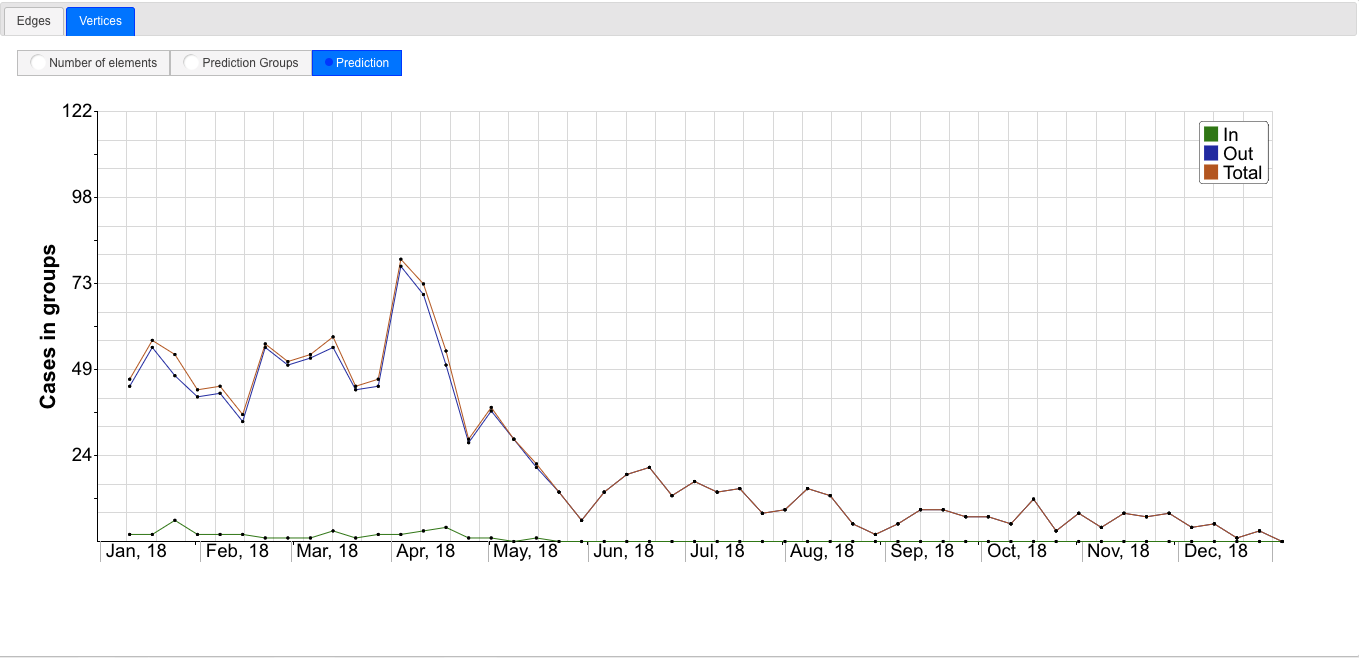
\includegraphics[width=15cm]{figuras/metricas/CHI_2018_4_500_1.png}
	}{
		\Fonte{Elaborado pelo autor}
	}
\end{figure}
\FloatBarrier

Outra forma de exibir os resultados das figuras anteriores é na forma de gráfico de colunas empilhadas, apresentados na seção \ref{ap:stdbscan}.

Devido aos problemas descritos na seção \ref{sec:modelo-st-ign} foram realizados diversos testes do ST-IGN variando o valor da distância máxima entre dois pontos. A pesquisa \cite{Salje2017} revela que a infecção do vírus da dengue acontece comumente em uma região próxima entre os casos analisados, onde 60\% dos casos de dengue que vivem a menos de 200 metros de distância são da mesma cadeia de transmissão, em oposição a 3\% dos casos separados por 1 a 5 quilômetros. Baseado nisso e nos resultados dos testes do ST-IGN, estabeleceu-se como distância máxima entre dois pontos o valor de 250 metros, a fim de encontrar o máximo de grupos formados pelo algoritmo.

As figuras a seguir apresentam gráficos sobre dengue e chikungunya, também nos anos de 2017 e 2018, levando em consideração as 4 semanas anteriores à semana do grupo de previsão e pelo menos 2 casos para caracterizar um grupo. As legendas indicam os casos dentro e fora de algum grupo de previsão, como descrito anteriormente. O cálculo do raio dos grupos de previsão é o mesmo usado no \acrshort{ST-DBSCAN}.


Assim como nos resultados do \acrshort{ST-DBSCAN}, a figura \ref{fig:metricasDengue201742501IGN} apresenta em média o número de casos fora de algum grupo de previsão maior que dentro de algum grupo de previsão.

\begin{figure}[!ht]
	\centering	
	\Caption{\label{fig:metricasDengue201742501IGN} Métricas ST-IGN: Dengue/2017, 4 semanas, Eps = 250m, MinPts = 2}
	\UECEfig{}{
		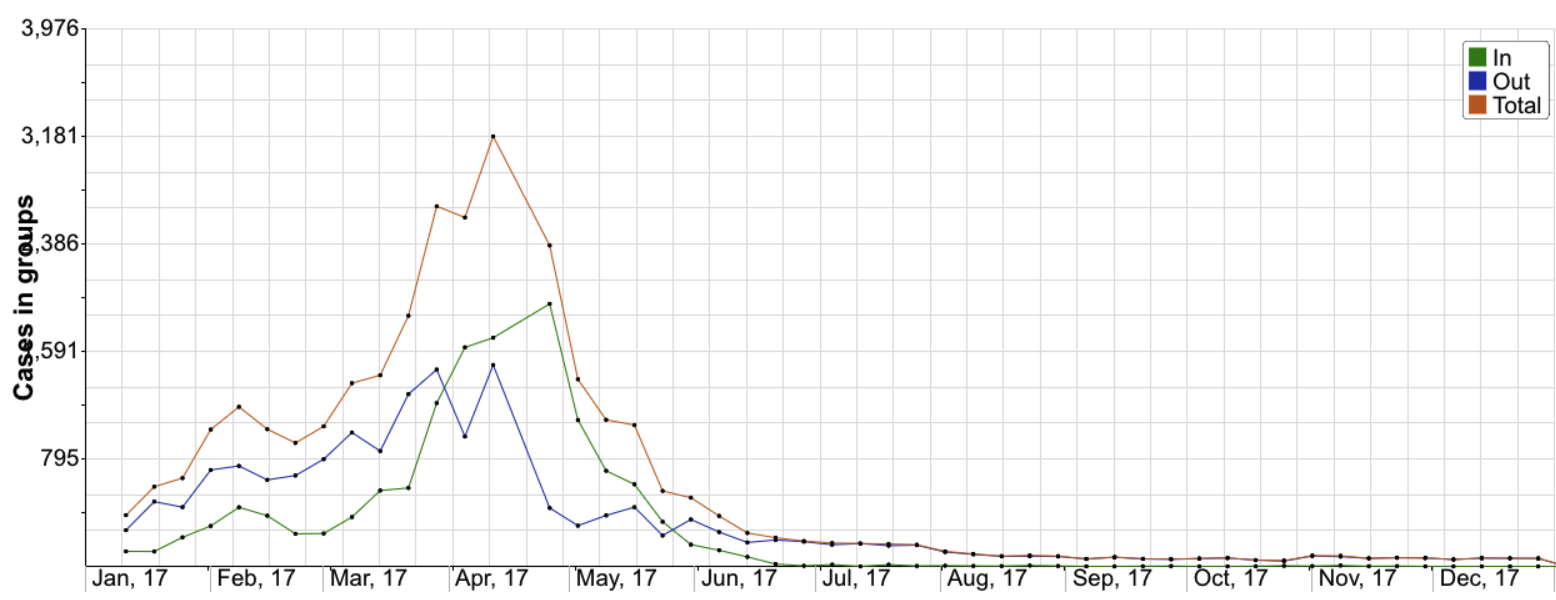
\includegraphics[width=15cm]{figuras/predicao/2017/Pred_ST-IGN_Dengue_2017_Cases.png}
	}{
		\Fonte{Elaborado pelo autor}
	}
\end{figure}
\FloatBarrier

Já a figura \ref{fig:metricasChi201742501IGN} apresenta uma grande quantidade de casos dentro de algum grupo de previsão ao longo do ano.
\begin{figure}[!ht]
	\centering	
	\Caption{\label{fig:metricasChi201742501IGN} Métricas ST-IGN: Chikungunya/2017, 4 semanas, Eps = 250m, MinPts = 2}
	\UECEfig{}{
		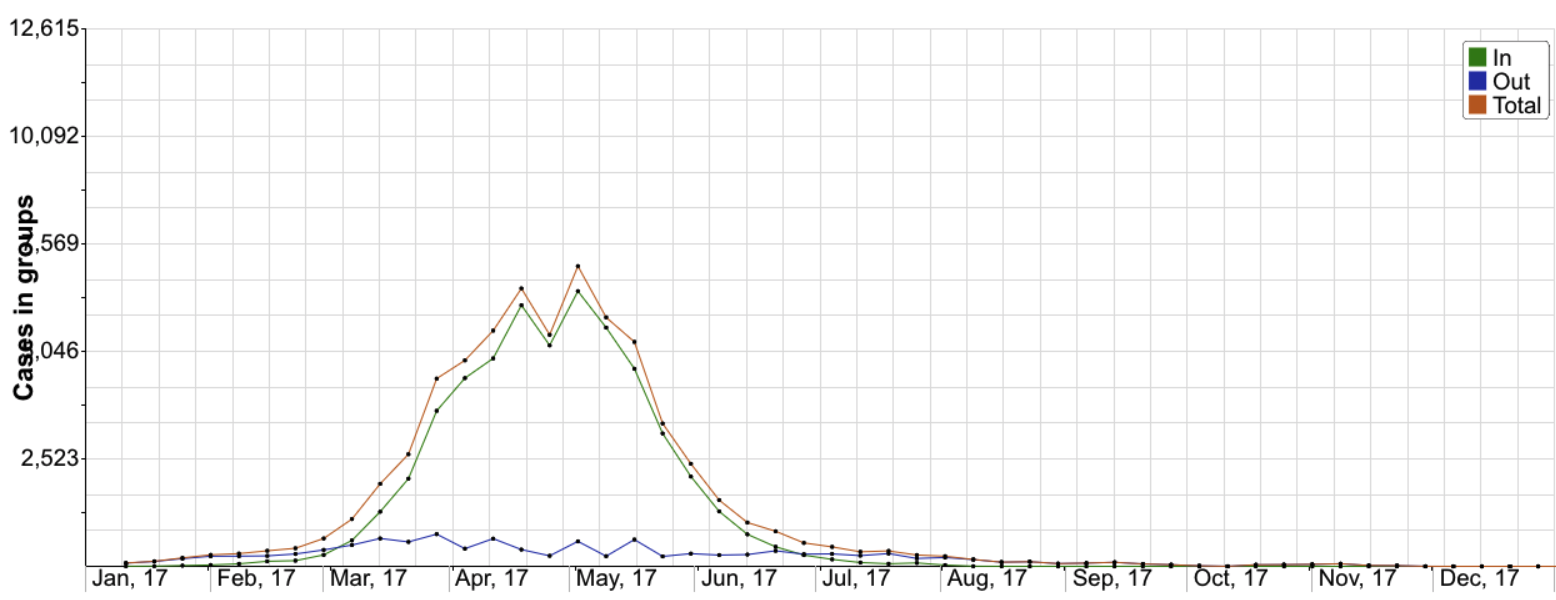
\includegraphics[width=15cm]{figuras/predicao/2017/Pred_ST-IGN_Chikungunya_2017_Cases.png}
	}{
		\Fonte{Elaborado pelo autor}
	}
\end{figure}
\FloatBarrier

Os resultados das figuras anteriores são exibidos na forma de gráfico de colunas empilhadas na seção \ref{ap:stign} do apêndice \ref{ap:graphicColBar}. 
Os resultados de chikungunya em 2018 foram praticamente nulos devido à baixa quantidade de casos, como mostra a figura \ref{fig:metricasChi201842501IGN}.



\subsection{Comparação dos resultados: ST-DBSCAN e ST-IGN}

A comparação exibida na figura \ref{fig:stdbscanstignweek6} foi feita para os casos de chikungunya na sexta semana de 2017, onde 1180 casos foram registrados, as semanas 2, 3, 4 e 5 foram analisadas e a distância máxima entre os casos num grupo foi de 250m. Os grupos de previsão do \acrshort{ST-DBSCAN} são representados pela cor vermelha, e os grupos de previsão do ST-IGN pela cor azul.
Pode-se observar na mesma figura que o \acrshort{ST-DBSCAN} encontrou mais grupos de previsão.

\begin{figure}[!ht]
	\centering	
	\Caption{\label{fig:stdbscanstignweek6} Comparação \acrshort{ST-DBSCAN} e ST-IGN: Chikungunya/2017, 4 semanas, Eps=250m, MinPts=2}
	\UECEfig{}{
		\includegraphics[width=15cm]{figuras/predicao/ST-DBSCAN_ST-IGN_week_6.png}
	}{
		\Fonte{Elaborado pelo autor}
	}
\end{figure}
\FloatBarrier

A tabela \ref{tab:stdbscanstign} mostra os resultados obtidos. Podemos destacar que o \acrshort{ST-DBSCAN} encontrou mais grupos de previsão, mas o ST-IGN encontra um maior percentual de grupos com pelo menos um caso.

\begin{table}[ht!]
	\centering
	\Caption{\label{tab:stdbscanstign} Resultados \acrshort{ST-DBSCAN} e ST-IGN: Chikungunya/2017}
	\UECEtab{}{
		\begin{tabular}{ccll}
			\toprule
	    		   & \acrshort{ST-DBSCAN} & ST-IGN \\
			\midrule \midrule
				Grupos de previsão & 205 & 136 \\
				Grupos com pelo menos um caso & 179 & 133 \\
				Casos Humanos dentro de algum grupo de previsão & 908 (77\%) & 656 (56\%) \\
				Casos Humanos fora de algum grupo de previsão & 272 (23\%) & 524 (44\%) \\
			\bottomrule
		\end{tabular}
	}{
		\Fonte{Elaborado pelo autor}
    }
\end{table}
\FloatBarrier

As tabelas \ref{tab:dengue20171} e \ref{tab:dengue20172} a seguir exibem um comparativo nas primeiras semanas do ano e aproximadamente dos percentuais de acerto dos grupos de previsão de Dengue/2017. Em média os resultados do algoritmo \acrshort{ST-DBSCAN} são mais acertivos. Esses mesmos resultados são exibidos como gráfico de colunas no apêndice \ref{ap:graphicColBar}.

\begin{table}[ht!]
	\centering
	\Caption{\label{tab:dengue20171} Resultados \acrshort{ST-DBSCAN} e ST-IGN: Dengue - 2017/1}
	\UECEtab{}{
		\begin{tabular}{cccccccccccccccll}
			\toprule
	    		Semana        &  1 &  2 &  3 &  4 &  5 &  6 &  7 &  8 &  9 & 10 & 11 & 12 & 13 & 14 & 15\\
			\midrule \midrule
				ST-IGN(\%)    & 29 & 18 & 32 & 29 & 37 & 37 & 26 & 23 & 27 & 40 & 32 & 45 & 62 & 53 & 81\\
				\acrshort{ST-DBSCAN}(\%) & 33 & 43 & 58 & 58 & 71 & 75 & 78 & 71 & 73 & 81 & 84 & 86 & 94 & 90 & 94\\
			\bottomrule
		\end{tabular}
	}{
		\Fonte{Elaborado pelo autor}
    }
\end{table}

\begin{table}[ht!]
	\centering
	\Caption{\label{tab:dengue20172} Resultados \acrshort{ST-DBSCAN} e ST-IGN: Dengue - 2017/2}
	\UECEtab{}{
		\begin{tabular}{cccccccccccccccll}
			\toprule
	    		Semana        & 16 & 17 & 18 & 19 & 20 & 21 & 22 & 23 & 24 & 25 & 26 & 27 & 28 & 29 & 30\\
			\midrule \midrule
				ST-IGN(\%)    & 78 & 65 & 58 & 59 & 31 & 32 & 28 &  8 &  4 &  8 &  0 & 13 &  2 &  5 &  4\\
				\acrshort{ST-DBSCAN}(\%) & 93 & 90 & 84 & 79 & 72 & 59 & 52 & 45 & 28 & 17 & 14 & 10 & 20 & 12 & 18\\
			\bottomrule
		\end{tabular}
	}{
		\Fonte{Elaborado pelo autor}
    }
\end{table}

\section{Resultados e Discussão}
\label{sec:discussao}
% discutir, interpretar e analisar os Resultados
Uma das vantagens apresentadas pelo método ST-IGN sobre o \acrshort{ST-DBSCAN} é a possibilidade de identificar grupos que não possuem uma forma regular, além da hiper-esférica (ou esférica/circular). Por isso, fez-se necessário a utilização de mais opções de parâmetros para a predição de casos de endemias (distância máxima entre os casos e número de semanas anteriores a semana em análise, por exemplo).


% Resultados:
As figuras \ref{fig:stdbscan2019dengue250} e \ref{fig:stdbscan2019chi250} apresentam gráficos sobre as ocorrências de casos humanos de dengue reportados em \cite{simda} no município de Fortaleza, no ano de 2019, levando em consideração as 4 semanas anteriores à semana do grupo de previsão. A variável Eps de agregação do \acrshort{ST-DBSCAN} e ST-IGN é de 250 metros e para caracterizar um grupo se considera pelo menos 2 casos humanos. A cor verde nos gráficos representa os casos dentro dos grupos de previsão e azul os casos fora. As ocorrências de casos de chikungunya em 2019 não foram significativas para analisar grupos de previsão espaço-temporal. Este resultado se assemelha as ocorrências de chikungunya em 2018 pelo número baixo de incidência de casos confirmados. A \ref{tab:casos} exibe o total de casos de dengue e chikungunya entre 2016 e até julho de 2019

\begin{table}[ht!]	
	\centering
	\Caption{\label{tab:casos} Total de casos de dengue e chikungunya}
	\UECEtab{}{
		\begin{tabular}{||c c c||}
			\toprule
	    		Doença & Dengue & Chikungunya \\
			\midrule \midrule
				2016 & 21853 & 17788 \\
				2017 & 13561 & 61727 \\
				2018 & 1417 & 577 \\
				2019(7/12) & 2119 & 158 \\
			\bottomrule
		\end{tabular}
	}{
		\Fonte{Elaborado pelo autor}
    }
\end{table}

% Figuras:
\begin{figure}[!ht]
	\centering	
	\Caption{\label{fig:stdbscan2019dengue250} \acrshort{ST-DBSCAN}: Dengue/2019, 4 semanas, Eps=250m, MinPts=2}
	\UECEfig{}{
		\includegraphics[width=15cm]{figuras/predicao/2019/Pred_ST-Dbscan_Dengue_2019_percent_250.png}
	}{
		\Fonte{Elaborado pelo autor}
	}
\end{figure}
\FloatBarrier

\begin{figure}[!ht]
	\centering	
	\Caption{\label{fig:stdbscan2019chi250} ST-IGN: Dengue/2019, 4 semanas, Eps=250m, MinPts=2}
	\UECEfig{}{
\includegraphics[width=15cm]{figuras/predicao/2019/Pred_ST-IGN_Dengue_2019_percent_250.png}
	}{
		\Fonte{Elaborado pelo autor}
	}
\end{figure}
\FloatBarrier

% TODO Discussão:


% ok    Incluir imagem com grupos dos dois algoritmos de uma semana qualquer e com relatórios ao lado
As figuras \ref{fig:resultadoSemana132017Comparativo} e \ref{fig:resultadoSemana132017} representam os resultados de predição espaço-temporal na semana 13 do ano de 2017, sobre ocorrência de casos humanos de dengue no algoritmo \acrshort{ST-DBSCAN}, onde a distância máxima entre dois pontos do mesmo grupo é de 250 metros e no algoritmo ST-IGN a distância máxima entre dois pontos, independente da distância entre os pontos do mesmo grupo, é também de 250 metros. Além disso, foram levados em consideração as 4 semanas anteriores à semana do grupo de previsão, e o número mínimo de 2 casos humanos para determinar um grupo. Foram registrados 2664 casos na semana em análise, onde 2299 casos foram encontrados dentro de algum grupo de previsão no ST-DBSCAN e 1926 casos pelo ST-IGN. Os grupos em azul foram gerados pelo ST-IGN e os grupos em vermelhor foram gerados pelo ST-DBSCAN, e também pode-se observar os grupos em rosa formados pela API do Google \emph{MarkerCluster} com o número de pontos por grupo representado pela nomeclatura G-\emph{n}, onde \emph{n} é o número de casos do grupo.

\begin{figure}[!ht]
	\centering	
	\Caption{\label{fig:resultadoSemana132017Comparativo} Resultados \acrshort{ST-DBSCAN} e ST-IGN: Dengue - 2017 Semana 13}
	\UECEfig{}{
\includegraphics[width=10cm]{figuras/DENGUE2017Semana13_250.png}
	}{
		\Fonte{Elaborado pelo autor}
	}
\end{figure}
\FloatBarrier

% Discussão:
Analisando os resultados da figura \ref{fig:resultadoSemana132017}, o \acrshort{ST-DBSCAN} destaca-se em relação ao ST-IGN em acertar mais casos dentro de algum grupo de previsão. Em contrapartida, o ST-IGN gera bem menos grupos de previsão e praticamente todos eles com pelo menos um caso.
Além disso, embora reconhecendo que são necessárias mais pesquisas para aplicar essas técnicas a outras fontes de dados sobre endemias, a fim de permitir uma avaliação abrangente de seus respectivos pontos fortes e limitações, acreditamos que a pesquisa realizada até o momento demonstrou que elas têm o potencial de fornecer soluções compreensíveis sobre a previsão de grupos de casos de endemias no espaço e no tempo.

\begin{figure}[!ht]
	\centering	
	\Caption{\label{fig:resultadoSemana132017} Resultados \acrshort{ST-DBSCAN} e ST-IGN: Dengue - 2017 Semana 13}
	\UECEfig{}{
\includegraphics[width=12cm]{figuras/DENGUE2017Semana13Algoritmos.png}
	}{
		\Fonte{Elaborado pelo autor}
	}
\end{figure}
\FloatBarrier
% TODO Discutir resultados mostrados nas figuras anteriores...


% TODO ____________________________________________
% Analisar qual o "melhor" algoritmo
% Descrever função objetivo e incluir nas discussões
% O ST-IGN apresenta melhores resultados se comparado ao ... Essa melhora é provocada pela alteração do eps tendo em vista que...
% Os resultados obtidos sugerem que...

% MELHORAR explicação da metodologia (imagem)

% ok Discussão em STCrime_ComparisonofMethods
% ok Discussão em GeoComputacionalSTAlgorithm_DENGUETAIWAN__NATURE_IMPORTANTE


	\chapter{Conclusões e Trabalhos Futuros}
\label{chap:conclusoes-e-trabalhos-futuros}

\section{Considerações finais}
\label{sec:contribuicoes-do-trabalho}

Criação de um método para resolver o Problema de Agrupamento em Grafos Dinâ-
micos e previsão de evolução destes agrupamentos.
A expectativa é de que ao final desta pesquisa, tenha-se uma extensão do Dynagraph
para visualização de agrupamentos dinâmicos e previsão dinâmica.
Utilizar a ferramenta para outros tipos de doenças como: Chikungunya e Zika Vírus.
Finalmente, espera-se que o produto final e os resultados obtidos possibilitem a previsão e
prevenção de novos casos de dengue para um combate efetivo à doença.

\section{Limitações}
\label{sec:limitacoes}

Dentre as dificuldades que podem interferir na execução deste projeto de pesquisa,
as seguintes podem ser citadas:
1. A escassez de estudos relacionando os assuntos abordados: agrupamento, previsão em
dados dinâmicos espaço-temporais, grafos dinâmicos e sistemas web de forma integrada;
2. Obtenção das informações dos focos e casos de dengue geolocalizadas e tempos das
ocorrências. A extração dos dados semanais requer um processo manual em \cite{simda},
pois é necessário o usuário selecionar o ano e a semana correspondente;
3. Visualização dos agrupamentos dinâmicos.
Para contornar as dificuldades apresentadas pretende-se:
1. Automatizar a forma de obtenção dos dados;
2. Utilizar o software Dynagraph como ambiente de suporte à validação e interação com os
resultados dos métodos de agrupamento espaço-temporal utilizados.

\section{Trabalhos Futuros}
\label{sec:trabalhos-futuros}

Em estudos futuros, pretende-se executar o algoritmo em paralelo, a fim de melhorar o desempenho, pois grandes bancos de dados necessitam de alto poder computacional. Além disso, heurísticas mais performáticas podem ser encontradas para determinar os parâmetros de entrada Eps e MinPts do ST-DBSCAN.




	
	%Elementos pós-textuais	
	\bibliography{elementos-pos-textuais/referencias}
    %\imprimirglossario	
	\imprimirapendices
		% Adicione aqui os apendices do seu trabalho
		\apendice{Tecnologias}
\label{ap:tecnologias}

A arquitetura do software foi desenvolvida em três partes: servidor, banco de dados e cliente. Tanto o lado cliente (\textit{frontend}) como o lado servidor (\textit{backend})
utilizam a linguagem Javascript.
Na parte do servidor, ou \textit{server-side}, foram utilizados Javascript (EcmaScript 6), NodeJS, Express e Mongoose. No lado do cliente foram utilizadas as seguintes tecnologias:
HTML, CSS, Javascript (EcmaScript 6), AngularJS e Dynagraph. O banco de dados MongoDB foi utilizado como suporte a leitura inicial dos dados.


\section{Servidor}
O \textit{backend} foi utilizado para manipular o banco de dados e transformar as informações na estrutura de dados do Dynagraph para permitir sua análise no \textit{frontend}.
O Node.js é uma plataforma de desenvolvimento para executar código Javascript no \textit{server-side} sobre o motor JavaScript do Google Chrome para facilmente construir aplicações de redes rápidas e escaláveis. Uma das maiores vantagens do Node.js é usar um modelo de I/O direcionada a evento não bloqueante que o torna leve e eficiente, ideal para aplicações em tempo real com troca intensa de dados através de dispositivos distribuídos.

O Express.js é um \textit{framework} JavaScript que facilita a criação de aplicativos web utilizando o Node.js e fornece um conjunto robusto de recursos para aplicativos web e móvel. Com vários métodos utilitários HTTP e \textit{middleware} disponíveis para criar uma API robusta, rápida e fácil. 

Mongoose é uma biblioteca do Nodejs que proporciona uma solução baseada em esquemas para modelar os dados da sua aplicação. Ele possui sistema de conversão de tipos, validação, criação de consultas e \textit{hooks} para lógica de negócios. Mongoose fornece um mapeamento de objetos do MongoDB similar ao ORM (Object Relational Mapping), ou ODM (Object Data Mapping) no caso do Mongoose. Isso significa que o Mongoose traduz os dados do banco de dados para objetos JavaScript para que possam ser utilizados por sua aplicação.

\section{Banco de dados}

MongoDB é um dos mais populares de banco de dados NoSQL. Ele é open-source, escrito em C++ e é um banco de dados orientado a documentos que armazena dados em documentos JSON com esquema dinâmico. Isso significa que você pode armazenar seus registros sem se preocupar com a estrutura de dados, como o número de campos ou tipos de campos para armazenar valores. Os documentos do MongoDB são semelhantes aos objetos JSON.

\section{Cliente}

%HTML
O HTML é uma Linguagem de Marcação de Hipertexto (\textit{Hypertext Markup Language}) utilizada para criar páginas web. Ele descreve a estrutura das páginas web usando marcadores (\textit{markup}). Os seus elementos são construídos em blocos de páginas HTML e são representados por \textit{tags}. Tags de HTML marcam partes de conteúdo, como "cabeçalho" (\textit{heading}), "parágrafo" (\textit{paragraph}), "tabela" (\textit{table}) e assim por diante. Os navegadores não exibem as tags HTML, mas as usam para renderizar o conteúdo da página \cite{html}.

%CSS
 Junto ao HTML temos o CSS (\textit{Cascading Style Sheets}), que é uma linguagem que descreve o estilo (\textit{style}) de um documento HTML. Além disso, ele descreve como os elementos HTML devem ser exibidos. Uma das vantagens em utilizar o CSS é controlar o \textit{layout} de múltiplas páginas web ao mesmo tempo. Ele é projetado para permitir a separação de apresentação e conteúdo, incluindo layout, cores e fontes. Essa separação pode melhorar a acessibilidade de conteúdo, fornecer mais flexibilidade e controle na especificação de características de apresentação e reduzir a complexidade e a repetição no conteúdo estrutural \cite{css}.

%Javascript
O JavaScript é uma linguagem de programação interpretada, frequentemente abreviado como JS, de alto nível, caracterizada como dinâmica, fracamente tipada, baseada em protótipos, de tipagem fraca.
O ECMAScript é uma linguagem de programação baseada em scripts, padronizada pela Ecma International na especificação ECMA-262. A linguagem é bastante usada em tecnologias para Internet, sendo esta base para a criação do JavaScript. A versão utilizada do ECMAScript para esta pesquisa foi a ECMAScript 6 ou ECMAScript2015 \cite{ecma2015}.

%JSON
Outro recurso associado ao \textit{frontend} é o JSON (\textit{JavaScript Object Notation}), que é um formato “leve” para troca de informações. Ele é baseado em um subconjunto da linguagem de programação JavaScript \cite{json} e também em dois tipos de estruturas: Coleção de pares chave/valor e lista ordenada de valores. As coleções de chave e valor são equivalentes a \textit{object}, \textit{record}, \textit{struct}, \textit{dictionary}, \textit{hash} e \textit{map} nas linguagens. As listas são equivalentes a \textit{array}, \textit{vector} ou \textit{list}.
Um objeto é um conjunto não ordenado de pares nome/valor. Um objeto começa com { (chave esquerda) e termina com } (chave direita). Cada nome é seguido por : (dois pontos) e os pares nome/valor são separados por , (vírgula).

%AngularJS
O Editor de Características foi incorporado ao Dynagraph após a sua conclusão, e o seu desenvolvimento foi realizado utilizando principalmente o \textit{framework} AngularJS \cite{angularjs}.
Este permite construir aplicações web dinâmicas e estender a sintaxe do HTML, e com isso simplifica o código e permite uma estrutura componentizada. A ligação de dados e a injeção de dependência do AngularJS eliminam grande parte do código que seria necessário escrever.
Seu principal padrão arquitetural é o MVC (\textit{Model View Controller}):
\begin{itemize}
	\item Modelo (\textit{Model}): são as propriedades de um escopo; escopos são anexados ao DOM onde as propriedades do escopo são acessadas por meio de ligações.
	\item Visão (\textit{View}): O \textit{template} (HTML com ligações de dados) que é renderizado na Visão.
	\item Controlador (\textit{Controller}): é a classe que contém a lógica de negócios por trás do aplicativo.
\end{itemize}

O HTML 5 traz consigo importantes mudanças em relação as últimas versões, através de novas funcionalidades como semântica e acessibilidade. Muitos dos seus recursos estão relacionados ao desenvolvimento do DYNAGRAPH.


\section{Arquitetura do Software}
A princípio o MongoDB foi utilizado para armazenar os dados salvos do \cite{simda}, a respeito da dengue e chikungunya. O cliente requisita os dados do servidor, que por sua vez processa as informações, seguindo a estrutura de dados do Dynagraph. Em seguida, esses dados processados são passados para a aplicação no cliente. Com os dados exibidos no browser podemos editá-los, gerar agrupamentos e finalmente salvar as informações em um arquivo no formato JSON, como mostra a arquitetura na figura \ref{fig:arqsoft}.

\begin{figure}[!ht]
	\centering	
	\Caption{\label{fig:arqsoft} Arquitetura do Softwate}	
	\UECEfig{}{
		\includegraphics[width=16cm]{figuras/apendice/dissertacaoArquitetura.png}
	}{
		\Fonte{Elaborado pelo autor}
	}
\end{figure}
\FloatBarrier

\section{Ferramentas e Materiais}
O desenvolvimento do trabalho foi realizado a partir dos seguintes equipamentos e materiais:
\begin{itemize}
	\item Macbook Pro 13" modelo 2015 / macOS High Sierra 10.13.2:
	\subitem Processador Intel Core i5 2.7 GHz;
	\subitem Memória de 8GB 1867 MHzs DDR3;
	\subitem HD SSD 128GB;
	\item Sistema Operacioal Mac OS High Sierra 10.13.2 e Windwows;
	\item Ambiente de desenvolvimento Webstorm;
	\item Navegador de internet Google Chrome 63.0.3239.132.
	\item Controle de versão Git (Software e dissertação);
	\item \LaTeX ${ }$ para produção da dissertação;
	\item Portal de periódicos CAPES, como principal fonte de pesquisa;
\end{itemize}
		\apendice{Gráfico de colunas empilhadas}
\label{ap:graphicColBar}

\section{ST-DBSCAN}
\label{ap:stdbscan}

Os resultados exibidos na figura \ref{fig:metricasChi201842501} foram quase nulos devido a baixa quantidade de casos de Chikungunya, e além disso os poucos casos são distantes, logo não atendem ao critério básico de distância máxima entre dois pontos para formar um grupo.
\begin{figure}[!ht]
	\centering	
	\Caption{\label{fig:metricasChi201842501} Métricas ST-DBSCAN: Chikungunya/2018, 4 semanas, Eps = 250, MinPts = 2}
	\UECEfig{}{
		\includegraphics[width=15cm]{figuras/metricas/ST-DBSCAN_2018.png}
	}{
		\Fonte{Elaborado pelo autor}
	}
\end{figure}

\pagebreak
\section{ST-IGN}
\label{ap:stign}

Os resultados em \ref{fig:metricasChi201842501IGN} também foram praticamente nulos devido a baixa quantidade de casos de Chikungunya, e distância máxima entre dois pontos para formar um grupo de 250 metros.
\begin{figure}[!ht]
	\centering	
	\Caption{\label{fig:metricasChi201842501IGN} Métricas ST-IGN: Chikungunya/2018, 4 semanas, Eps = 250, MinPts = 2}
	\UECEfig{}{
		\includegraphics[width=15cm]{figuras/metricas/ST-IGN_2018.png}
	}{
		\Fonte{Elaborado pelo autor}
	}
\end{figure}
\FloatBarrier

\begin{sidewaysfigure}[!ht]
	\centering
	\Caption{\label{fig:metricasDengueBar201745001} Métricas ST-DBSCAN: Dengue/2017, 4 semanas, Eps = 500m, MinPts = 2}
	\UECEfig{}{
		\includegraphics[width=25cm]{figuras/metricas/dengue2017chartbar.png}
	}{
		\Fonte{Elaborado pelo autor}
	}
\end{sidewaysfigure}


\begin{sidewaysfigure}[!ht]
	\centering	
	\Caption{\label{fig:metricasDengueBar201845001} Métricas ST-DBSCAN: Dengue/2018, 4 semanas, Eps = 500m, MinPts = 2}
	\UECEfig{}{
		\includegraphics[width=25cm]{figuras/metricas/dengue2018chartbar.png}
	}{
		\Fonte{Elaborado pelo autor}
	}
\end{sidewaysfigure}


\begin{sidewaysfigure}[!ht]
	\centering	
	\Caption{\label{fig:metricasChi201745002} Métricas ST-DBSCAN: Chikungunya/2017, 4 semanas, Eps = 500m, MinPts = 2}
	\UECEfig{}{
		\includegraphics[width=25cm]{figuras/metricas/chikungunya2017chartbar.png}
	}{
		\Fonte{Elaborado pelo autor}
	}
\end{sidewaysfigure}

\begin{sidewaysfigure}[!ht]
	\centering	
	\Caption{\label{fig:metricasChi201742502} Métricas ST-DBSCAN: Chikungunya/2017, 4 semanas, Eps = 250m, MinPts = 2}
	\UECEfig{}{
		\includegraphics[width=25cm]{figuras/predicao/2017/Pred_ST-Dbscan_Chikungunya_2017_percent.png}
	}{
		\Fonte{Elaborado pelo autor}
	}
\end{sidewaysfigure}


\begin{sidewaysfigure}[!ht]
	\centering
	\Caption{\label{fig:metricasChi201742502IGN} Métricas ST-IGN: Chikungunya/2017, 4 semanas, Eps = 250, MinPts = 2}
	\UECEfig{}{
		\includegraphics[width=25cm]{figuras/predicao/2017/Pred_ST-IGN_Chikungunya_2017_percent.png}
	}{
		\Fonte{Elaborado pelo autor}
	}
\end{sidewaysfigure}

\begin{sidewaysfigure}[!ht]
	\centering
	\Caption{\label{fig:metricasDen201742502IGN} Métricas ST-IGN: Dengue/2017, 4 semanas, Eps = 250, MinPts = 2}
	\UECEfig{}{
		\includegraphics[width=25cm]{figuras/predicao/2017/Pred_ST-IGN_Dengue_2017_percent.png}
	}{
		\Fonte{Elaborado pelo autor}
	}
\end{sidewaysfigure}

\begin{sidewaysfigure}[!ht]
	\centering
	\Caption{\label{fig:metricasDen201842502IGN} Métricas ST-IGN: Dengue/2018, 4 semanas, Eps = 250, MinPts = 2}
	\UECEfig{}{
		\includegraphics[width=25cm]{figuras/predicao/2018/Pred_ST-IGN_Dengue_2018_percent.png}
	}{
		\Fonte{Elaborado pelo autor}
	}
\end{sidewaysfigure}

	%\imprimiranexos
		% Adicione aqui os anexos do seu trabalho
	%	\anexo{Exemplo de Anexo}
\label{an:exemplo-de-anexo}

\lipsum[13]		
	%	\anexo{Dinâmica das classes sociais}
\label{an:dinamica-das-classes-sociais}

\lipsum[14]
\index{AAA}
	%\imprimirindice

\end{document}